\documentclass[twoside]{book}

% Packages required by doxygen
\usepackage{fixltx2e}
\usepackage{calc}
\usepackage{doxygen}
\usepackage[export]{adjustbox} % also loads graphicx
\usepackage{graphicx}
\usepackage[utf8]{inputenc}
\usepackage{makeidx}
\usepackage{multicol}
\usepackage{multirow}
\PassOptionsToPackage{warn}{textcomp}
\usepackage{textcomp}
\usepackage[nointegrals]{wasysym}
\usepackage[table]{xcolor}

% Font selection
\usepackage[T1]{fontenc}
\usepackage[scaled=.90]{helvet}
\usepackage{courier}
\usepackage{amssymb}
\usepackage{sectsty}
\renewcommand{\familydefault}{\sfdefault}
\allsectionsfont{%
  \fontseries{bc}\selectfont%
  \color{darkgray}%
}
\renewcommand{\DoxyLabelFont}{%
  \fontseries{bc}\selectfont%
  \color{darkgray}%
}
\newcommand{\+}{\discretionary{\mbox{\scriptsize$\hookleftarrow$}}{}{}}

% Page & text layout
\usepackage{geometry}
\geometry{%
  a4paper,%
  top=2.5cm,%
  bottom=2.5cm,%
  left=2.5cm,%
  right=2.5cm%
}
\tolerance=750
\hfuzz=15pt
\hbadness=750
\setlength{\emergencystretch}{15pt}
\setlength{\parindent}{0cm}
\setlength{\parskip}{3ex plus 2ex minus 2ex}
\makeatletter
\renewcommand{\paragraph}{%
  \@startsection{paragraph}{4}{0ex}{-1.0ex}{1.0ex}{%
    \normalfont\normalsize\bfseries\SS@parafont%
  }%
}
\renewcommand{\subparagraph}{%
  \@startsection{subparagraph}{5}{0ex}{-1.0ex}{1.0ex}{%
    \normalfont\normalsize\bfseries\SS@subparafont%
  }%
}
\makeatother

% Headers & footers
\usepackage{fancyhdr}
\pagestyle{fancyplain}
\fancyhead[LE]{\fancyplain{}{\bfseries\thepage}}
\fancyhead[CE]{\fancyplain{}{}}
\fancyhead[RE]{\fancyplain{}{\bfseries\leftmark}}
\fancyhead[LO]{\fancyplain{}{\bfseries\rightmark}}
\fancyhead[CO]{\fancyplain{}{}}
\fancyhead[RO]{\fancyplain{}{\bfseries\thepage}}
\fancyfoot[LE]{\fancyplain{}{}}
\fancyfoot[CE]{\fancyplain{}{}}
\fancyfoot[RE]{\fancyplain{}{\bfseries\scriptsize Generated by Doxygen }}
\fancyfoot[LO]{\fancyplain{}{\bfseries\scriptsize Generated by Doxygen }}
\fancyfoot[CO]{\fancyplain{}{}}
\fancyfoot[RO]{\fancyplain{}{}}
\renewcommand{\footrulewidth}{0.4pt}
\renewcommand{\chaptermark}[1]{%
  \markboth{#1}{}%
}
\renewcommand{\sectionmark}[1]{%
  \markright{\thesection\ #1}%
}

% Indices & bibliography
\usepackage{natbib}
\usepackage[titles]{tocloft}
\setcounter{tocdepth}{3}
\setcounter{secnumdepth}{5}
\makeindex

% Hyperlinks (required, but should be loaded last)
\usepackage{ifpdf}
\ifpdf
  \usepackage[pdftex,pagebackref=true]{hyperref}
\else
  \usepackage[ps2pdf,pagebackref=true]{hyperref}
\fi
\hypersetup{%
  colorlinks=true,%
  linkcolor=blue,%
  citecolor=blue,%
  unicode%
}

% Custom commands
\newcommand{\clearemptydoublepage}{%
  \newpage{\pagestyle{empty}\cleardoublepage}%
}

\usepackage{caption}
\captionsetup{labelsep=space,justification=centering,font={bf},singlelinecheck=off,skip=4pt,position=top}

%===== C O N T E N T S =====

\begin{document}

% Titlepage & ToC
\hypersetup{pageanchor=false,
             bookmarksnumbered=true,
             pdfencoding=unicode
            }
\pagenumbering{alph}
\begin{titlepage}
\vspace*{7cm}
\begin{center}%
{\Large Pa\+Sca\+L\+\_\+\+T\+D\+M\+A2.0 }\\
\vspace*{1cm}
{\large Generated by Doxygen 1.8.13}\\
\end{center}
\end{titlepage}
\clearemptydoublepage
\pagenumbering{roman}
\tableofcontents
\clearemptydoublepage
\pagenumbering{arabic}
\hypersetup{pageanchor=true}

%--- Begin generated contents ---
\chapter{Pa\+Sca\+L\+\_\+\+T\+D\+MA 2.0}
\label{md__home_jihoon__develop__pa_sca_l__t_d_m_a__r_e_a_d_m_e}
\Hypertarget{md__home_jihoon__develop__pa_sca_l__t_d_m_a__r_e_a_d_m_e}
Parallel and Scalable Library for Tri\+Diagonal Matrix Algorithm

Pa\+Scal\+\_\+\+T\+D\+MA provides an efficient and scalable computational procedure to solve many tridiagonal systems in multi-\/dimensional partial differential equations. The modified Thomas algorithm proposed by Laszlo et al.(2016) and the newly designed communication scheme have been used to reduce the communication overhead in solving many tridiagonal systems.

This library is for both single and many tridiagonal systems of equations. The main algorithm for a tridiagonal matrix consists of the following five steps\+:


\begin{DoxyItemize}
\item (1) Transform the partitioned submatrices in the tridiagonal systems into modified submatrices\+: Each computing core transforms the partitioned submatrices in the tridiagonal systems of equations into the modified forms by applying modified Thomas algorithm.
\item (2) Construct reduced tridiagonal systems from the modified submatrices\+: The reduced tridiagonal systems are constructed by collecting the first and last rows of the modified submatrices from each core using M\+P\+I\+\_\+\+Ialltoallw.
\item (3) Solve the reduced tridiagonal systems\+: The reduced tridiagonal systems constructed in Step 2 are solved by applying the Thomas algorithm.
\item (4) Distribute the solutions of the reduced tridiagonal systems\+: The solutions of the reduced tridiagonal systems in Step 3 are distributed to each core using M\+P\+I\+\_\+\+Ialltoallw. This communication is an exact inverse of the communication in Step 2.
\item (5) Update the other unknowns in the modified tridiagonal systems\+: The remaining unknowns in the modified submatrices in Step 1 are solved in each computing core with the solutions obtained in Step 3 and Step 4.
\end{DoxyItemize}

Step 1 and Step 5 are similar to the method proposed by Laszlo et al.(2016) which uses parallel cyclic reduction (P\+CR) algorithm to build and solve the reduced tridiagonal systems. Instead of using the P\+CR, we develop an all-\/to-\/all communication scheme using the M\+P\+I\+\_\+\+Ialltoall function after the modified Thomas algorithm is executed. The number of coefficients for the reduced tridiagonal systems are greatly reduced, so we can avoid the communication bandwidth problem, which is a main bottleneck for all-\/to-\/all communications. Our algorithm is also distinguished from the work of Mattor et al. (1995) which assembles the undetermined coefficients of the temporary solutions in a single processor using M\+P\+I\+\_\+\+Gather, where load imbalances are serious.

\section*{C\+U\+DA implementation in Pa\+Scal\+\_\+\+T\+D\+MA 2.\+0}

In Pa\+Sca\+L\+\_\+\+T\+D\+MA 2.\+0, multi-\/\+G\+PU acceleration is implemented using N\+V\+I\+D\+IA C\+U\+DA. C\+U\+D\+A-\/related features are as follows\+:
\begin{DoxyItemize}
\item (1) Incorporation of C\+U\+DA kernels into the loop structures of the existing algorithm, that are modified to exploit more G\+PU threads.
\item (2) Utilization of shared memory using pipeline copy of variables in device memory to reduce the amount of device memory access.
\item (3) C\+U\+D\+A-\/aware M\+PI communication for rapid communication with the support of hardward
\item (4) Use of 3\+D-\/array for practical applications and accordingly the use of C\+U\+DA threads more than in a single dimension with the 3-\/D array.
\item (5) Depreciation on functions for single tridiagonal matrix as they are rarely used for three-\/dimensional problems.
\end{DoxyItemize}

\section*{Authors}


\begin{DoxyItemize}
\item Kiha Kim (\href{mailto:k-kiha@yonsei.ac.kr}{\tt k-\/kiha@yonsei.\+ac.\+kr}), Multi-\/\+Physics Modeling and Computation Lab., Yonsei University
\item Mingyu Yang (\href{mailto:yang926@yonsei.ac.kr}{\tt yang926@yonsei.\+ac.\+kr}), Multi-\/\+Physics Modeling and Computation Lab., Yonsei University
\item Ji-\/\+Hoon Kang (\href{mailto:jhkang@kisti.re.kr}{\tt jhkang@kisti.\+re.\+kr}), Korea Institute of Science and Technology Information
\item Jung-\/\+Il Choi (\href{mailto:jic@yonsei.ac.kr}{\tt jic@yonsei.\+ac.\+kr}), Multi-\/\+Physics Modeling and Computation Lab., Yonsei University
\end{DoxyItemize}

\section*{Usage}

\subsection*{Downloading Pa\+Sca\+L\+\_\+\+T\+D\+MA}

The repository can be cloned as follows\+:


\begin{DoxyCode}
git clone https://github.com/MPMC-Lab/PaScaL\_TDMA.git
\end{DoxyCode}
 Alternatively, the source files can be downloaded through github menu \textquotesingle{}Download Z\+IP\textquotesingle{}.

\subsection*{Compile}

\subsubsection*{Prerequisites}

Prerequisites to compile Pa\+Sca\+L\+\_\+\+T\+D\+M\+AS are as follows\+:
\begin{DoxyItemize}
\item M\+PI
\item fortran compiler (`nvfortran for G\+PU runs, N\+V\+I\+D\+IA H\+PC S\+KD 21.\+1 or higher)
\end{DoxyItemize}

\subsubsection*{Compile and build}


\begin{DoxyItemize}
\item Build Pa\+Sca\+L\+\_\+\+T\+D\+MA ``` make lib ```
\item Build an example problem after build Pa\+Sca\+L\+\_\+\+T\+D\+MA

``` make example ```
\item Build all

``` make all ``` \subsubsection*{Mores on compile option}

The {\ttfamily Makefile} in root directory is to compile the source code, and is expected to work for most systems. The \textquotesingle{}\hyperlink{_makefile_8inc}{Makefile.\+inc}\textquotesingle{} file in the root directory can be used to change the compiler (and M\+PI wrapper) and a few pre-\/defined compile options depending on compiler, execution environment and et al.
\end{DoxyItemize}

\subsection*{Running the example}

After building the example file, an executable binary, {\ttfamily a.\+out}, is built in the {\ttfamily run} folder. The {\ttfamily P\+A\+R\+A\+\_\+\+I\+N\+P\+U\+T.\+inp} file in the {\ttfamily run} folder is a pre-\/defined input file, and the {\ttfamily a.\+out} can be executed as follows\+: ``` mpirun -\/np 8 ./a.out ./\+P\+A\+R\+A\+\_\+\+I\+N\+P\+UT.inp ```

\section*{Folder structure}


\begin{DoxyItemize}
\item {\ttfamily src} \+: source files of Pa\+Sca\+L\+\_\+\+T\+D\+M\+A\+\_\+\+C\+U\+DA.
\item {\ttfamily example} \+: source files of an example problem for 3D heat-\/transfer equation.
\item {\ttfamily include} \+: header files are created after building
\item {\ttfamily lib} \+: a static library of Pa\+Sca\+L\+\_\+\+T\+D\+M\+A\+\_\+\+C\+U\+DA is are created after building
\item {\ttfamily doc} \+: documentation
\item {\ttfamily run} \+: an executable binary file for the example problem is created after building.
\end{DoxyItemize}

\section*{Cite}

Please use the following bibtex, when you refer to this project. \begin{DoxyVerb}@article{kkpc2020,
    title = "PaScaL_TDMA: A library of parallel and scalable solvers for massive tridiagonal system",
    author = "Kim, Kiha and Kang, Ji-Hoon and Pan, Xiaomin and Choi, Jung-Il",
    journal = "Computer Physics Communications",
    volume = "260",
    pages = "107722",
    year = "2021",
    issn = "0010-4655",
    doi = "https://doi.org/10.1016/j.cpc.2020.107722"
}

@misc{PaScaL_TDMA2019,
    title  = "Parallel and Scalable Library for TriDiagonal Matrix Algorithm",
    author = "Kim, Kiha and Kang, Ji-Hoon and Choi, Jung-Il",
    url    = "https://github.com/MPMC-Lab/PaScaL_TDMA",
    year   = "2019"
}
\end{DoxyVerb}


\section*{References}

For more information, please the reference paper and \href{https://www.mpmc.yonsei.ac.kr/}{\tt Multi-\/\+Physics Modeling and Computation Lab.} 
\chapter{Modules Index}
\section{Modules List}
Here is a list of all modules with brief descriptions\+:\begin{DoxyCompactList}
\item\contentsline{section}{\hyperlink{namespaceglobal}{global} \\*Module for global parameters }{\pageref{namespaceglobal}}{}
\item\contentsline{section}{\hyperlink{namespacempi__subdomain}{mpi\+\_\+subdomain} \\*Module for building subdomains from the physical domain }{\pageref{namespacempi__subdomain}}{}
\item\contentsline{section}{\hyperlink{namespacempi__topology}{mpi\+\_\+topology} \\*Module for creating the cartesian topology of the M\+PI processes and subcommunicators }{\pageref{namespacempi__topology}}{}
\item\contentsline{section}{\hyperlink{namespacenvtx}{nvtx} }{\pageref{namespacenvtx}}{}
\item\contentsline{section}{\hyperlink{namespacepascal__tdma}{pascal\+\_\+tdma} \\*Module for Pa\+Sca\+L-\/\+T\+D\+MA library }{\pageref{namespacepascal__tdma}}{}
\item\contentsline{section}{\hyperlink{namespacesolve__theta}{solve\+\_\+theta} }{\pageref{namespacesolve__theta}}{}
\end{DoxyCompactList}

\chapter{Data Type Index}
\section{Data Types List}
Here are the data types with brief descriptions\+:\begin{DoxyCompactList}
\item\contentsline{section}{\hyperlink{structmpi__topology_1_1cart__comm__1d}{mpi\+\_\+topology\+::cart\+\_\+comm\+\_\+1d} \\*Type variable for the information of 1D communicator }{\pageref{structmpi__topology_1_1cart__comm__1d}}{}
\item\contentsline{section}{\hyperlink{structnvtx_1_1nvtxeventattributes}{nvtx\+::nvtxeventattributes} }{\pageref{structnvtx_1_1nvtxeventattributes}}{}
\item\contentsline{section}{\hyperlink{interfacenvtx_1_1nvtxrangepop}{nvtx\+::nvtxrangepop} }{\pageref{interfacenvtx_1_1nvtxrangepop}}{}
\item\contentsline{section}{\hyperlink{interfacenvtx_1_1nvtxrangepush}{nvtx\+::nvtxrangepush} }{\pageref{interfacenvtx_1_1nvtxrangepush}}{}
\item\contentsline{section}{\hyperlink{structpascal__tdma_1_1ptdma__plan__many}{pascal\+\_\+tdma\+::ptdma\+\_\+plan\+\_\+many} \\*Execution plan for many tridiagonal systems of equations }{\pageref{structpascal__tdma_1_1ptdma__plan__many}}{}
\item\contentsline{section}{\hyperlink{structpascal__tdma_1_1ptdma__plan__single}{pascal\+\_\+tdma\+::ptdma\+\_\+plan\+\_\+single} \\*Execution plan for a single tridiagonal system of equations }{\pageref{structpascal__tdma_1_1ptdma__plan__single}}{}
\end{DoxyCompactList}

\chapter{File Index}
\section{File List}
Here is a list of all files with brief descriptions\+:\begin{DoxyCompactList}
\item\contentsline{section}{/home/jihoon/\+Develop/\+Pa\+Sca\+L\+\_\+\+T\+D\+M\+A/\hyperlink{_makefile_8inc}{Makefile.\+inc} }{\pageref{_makefile_8inc}}{}
\item\contentsline{section}{/home/jihoon/\+Develop/\+Pa\+Sca\+L\+\_\+\+T\+D\+M\+A/examples/\hyperlink{global_8f90}{global.\+f90} \\*This file contains a module of global parameters for the example problem of Pa\+Sca\+L\+\_\+\+T\+D\+MA }{\pageref{global_8f90}}{}
\item\contentsline{section}{/home/jihoon/\+Develop/\+Pa\+Sca\+L\+\_\+\+T\+D\+M\+A/examples/\hyperlink{main_8f90}{main.\+f90} \\*This file contains the main subroutines for an example problem of Pa\+Sca\+L\+\_\+\+T\+D\+MA }{\pageref{main_8f90}}{}
\item\contentsline{section}{/home/jihoon/\+Develop/\+Pa\+Sca\+L\+\_\+\+T\+D\+M\+A/examples/\hyperlink{mpi__subdomain_8f90}{mpi\+\_\+subdomain.\+f90} \\*This file contains a module of subdomains for the example problem of Pa\+Sca\+L\+\_\+\+T\+D\+MA }{\pageref{mpi__subdomain_8f90}}{}
\item\contentsline{section}{/home/jihoon/\+Develop/\+Pa\+Sca\+L\+\_\+\+T\+D\+M\+A/examples/\hyperlink{mpi__topology_8f90}{mpi\+\_\+topology.\+f90} \\*This file contains a module of communication topology for the example problem of Pa\+Sca\+L\+\_\+\+T\+D\+MA }{\pageref{mpi__topology_8f90}}{}
\item\contentsline{section}{/home/jihoon/\+Develop/\+Pa\+Sca\+L\+\_\+\+T\+D\+M\+A/examples/\hyperlink{solve__theta_8f90}{solve\+\_\+theta.\+f90} \\*This file contains a solver subroutine for the example problem of Pa\+Sca\+L\+\_\+\+T\+D\+MA }{\pageref{solve__theta_8f90}}{}
\item\contentsline{section}{/home/jihoon/\+Develop/\+Pa\+Sca\+L\+\_\+\+T\+D\+M\+A/src/\hyperlink{nvtx_8f90}{nvtx.\+f90} }{\pageref{nvtx_8f90}}{}
\item\contentsline{section}{/home/jihoon/\+Develop/\+Pa\+Sca\+L\+\_\+\+T\+D\+M\+A/src/\hyperlink{para__range_8f90}{para\+\_\+range.\+f90} \\*The para\+\_\+range function assigns the computing range to each M\+PI process }{\pageref{para__range_8f90}}{}
\item\contentsline{section}{/home/jihoon/\+Develop/\+Pa\+Sca\+L\+\_\+\+T\+D\+M\+A/src/\hyperlink{pascal__tdma_8f90}{pascal\+\_\+tdma.\+f90} \\*Pa\+Sca\+L\+\_\+\+T\+D\+MA -\/ Parallel and Scalable Library for Tri\+Diagonal Matrix Algorithm }{\pageref{pascal__tdma_8f90}}{}
\item\contentsline{section}{/home/jihoon/\+Develop/\+Pa\+Sca\+L\+\_\+\+T\+D\+M\+A/src/\hyperlink{tdmas_8f90}{tdmas.\+f90} \\*Tridiagonal matrix (T\+DM) solvers using the Thomas algorithm }{\pageref{tdmas_8f90}}{}
\end{DoxyCompactList}

\chapter{Module Documentation}
\hypertarget{namespaceglobal}{}\section{global Module Reference}
\label{namespaceglobal}\index{global@{global}}


Module for global parameters.  


\subsection*{Functions/\+Subroutines}
\begin{DoxyCompactItemize}
\item 
subroutine \hyperlink{namespaceglobal_a930b565da2644b675f35b91735e11ce3}{global\+\_\+inputpara} (np\+\_\+dim)
\begin{DoxyCompactList}\small\item\em Assign global parameters. \end{DoxyCompactList}\end{DoxyCompactItemize}
\subsection*{Variables}
\begin{DoxyCompactItemize}
\item 
double precision, parameter \hyperlink{namespaceglobal_a2eeeef6cb4401e0205ced808c718dead}{pi} = acos(-\/1.d0)
\item 
double precision \hyperlink{namespaceglobal_a31749f11f262d021576cd0d09bdc79c2}{pr}
\begin{DoxyCompactList}\small\item\em Prandtl number. \end{DoxyCompactList}\item 
double precision \hyperlink{namespaceglobal_a7b363950bb58d4e52dda12a928b2b9e2}{ra}
\begin{DoxyCompactList}\small\item\em Reyleigh number. \end{DoxyCompactList}\item 
integer \hyperlink{namespaceglobal_ac8816f9dd096716fb9b7e61d57cc5189}{tmax}
\begin{DoxyCompactList}\small\item\em Maximum number of iteration steps. \end{DoxyCompactList}\item 
double precision \hyperlink{namespaceglobal_a24d27ecfb0e7d422997122c9345bac8b}{dt}
\begin{DoxyCompactList}\small\item\em Length of time step. \end{DoxyCompactList}\item 
double precision \hyperlink{namespaceglobal_a3c8fbc22da61f7188e79bad2b9ba1d16}{dtstart}
\begin{DoxyCompactList}\small\item\em Initial dt. \end{DoxyCompactList}\item 
double precision \hyperlink{namespaceglobal_a07363365436fd22a91cdb5a847b4bb88}{tstart}
\begin{DoxyCompactList}\small\item\em Initial simulation time. \end{DoxyCompactList}\item 
double precision \hyperlink{namespaceglobal_a367640054e0083add94204f1a61bd61a}{theta\+\_\+cold}
\begin{DoxyCompactList}\small\item\em Boundary temperature of cold wall. \end{DoxyCompactList}\item 
double precision \hyperlink{namespaceglobal_a63b846fbcd5aedd45f92a0b1eb972244}{theta\+\_\+hot}
\begin{DoxyCompactList}\small\item\em Boundary temperature of hot wall. \end{DoxyCompactList}\item 
double precision \hyperlink{namespaceglobal_abe54a711bf9d8c30a6debfb651bdf47d}{alphag}
\begin{DoxyCompactList}\small\item\em Thermal expansion coefficient x gravitational acceleration. \end{DoxyCompactList}\item 
double precision \hyperlink{namespaceglobal_a48babc9c7f07053917ca1392e7a7b721}{nu}
\begin{DoxyCompactList}\small\item\em Kinematic viscosity. \end{DoxyCompactList}\item 
double precision \hyperlink{namespaceglobal_acf5521de662915885b6a73718cd6314b}{ct}
\begin{DoxyCompactList}\small\item\em Thermal diffusivity. \end{DoxyCompactList}\item 
integer \hyperlink{namespaceglobal_a33db542cca17d8c3a156e90d31d8abe5}{thread\+\_\+in\+\_\+x}
\item 
integer \hyperlink{namespaceglobal_a2694e42b57b63e348f472d5a59bfe0fb}{thread\+\_\+in\+\_\+y}
\item 
integer \hyperlink{namespaceglobal_a1f39f066a0ed398d1e3e56d13d092718}{thread\+\_\+in\+\_\+z}
\item 
integer \hyperlink{namespaceglobal_a0c53f9dfde5486b01023d0c9479db29c}{thread\+\_\+in\+\_\+x\+\_\+pascal}
\item 
integer \hyperlink{namespaceglobal_af395b143d44c9d28517e64a695920dda}{thread\+\_\+in\+\_\+y\+\_\+pascal}
\end{DoxyCompactItemize}
\textbf{ }\par
\begin{DoxyCompactItemize}
\item 
integer \hyperlink{namespaceglobal_a4ba10a6dbbcebb68e0d5e36a6c291898}{nx}
\begin{DoxyCompactList}\small\item\em Grid numbers in each direction. \end{DoxyCompactList}\item 
integer \hyperlink{namespaceglobal_a12dd7ca24c7675f31e6de07b1769991c}{ny}
\item 
integer \hyperlink{namespaceglobal_ab8d7436a6037d4c1b7248107a2f07d76}{nz}
\end{DoxyCompactItemize}

\textbf{ }\par
\begin{DoxyCompactItemize}
\item 
integer \hyperlink{namespaceglobal_aa37f5fe09139707ac1723302127436b1}{nxm}
\begin{DoxyCompactList}\small\item\em Grid numbers minus 1 in each direction. \end{DoxyCompactList}\item 
integer \hyperlink{namespaceglobal_a9852876e90514ccc182c0ed0b27cdaad}{nym}
\item 
integer \hyperlink{namespaceglobal_a76e27e2001870f6606e51d33a2c70f60}{nzm}
\end{DoxyCompactItemize}

\textbf{ }\par
\begin{DoxyCompactItemize}
\item 
integer \hyperlink{namespaceglobal_a227001d8177d0295b61a39948436adaa}{nxp}
\begin{DoxyCompactList}\small\item\em Grid numbers plus 1 in each direction. \end{DoxyCompactList}\item 
integer \hyperlink{namespaceglobal_a868bbe46b97daa7ff6c962fff16bbf2f}{nyp}
\item 
integer \hyperlink{namespaceglobal_ab376cd7d790b630ad83ffcded3c56366}{nzp}
\end{DoxyCompactItemize}

\textbf{ }\par
\begin{DoxyCompactItemize}
\item 
double precision \hyperlink{namespaceglobal_ac5d2ea39fc192fbb8354e665dc91b759}{lx}
\begin{DoxyCompactList}\small\item\em Lengths of the physical domain. \end{DoxyCompactList}\item 
double precision \hyperlink{namespaceglobal_a6a6ee40bbab9e114aa217f7d8570b924}{ly}
\item 
double precision \hyperlink{namespaceglobal_a9d90050855b894304d8b4272c6a9ee71}{lz}
\end{DoxyCompactItemize}

\textbf{ }\par
\begin{DoxyCompactItemize}
\item 
double precision \hyperlink{namespaceglobal_a9c5f8c3cf5f9b496608059fc13776b4c}{dx}
\begin{DoxyCompactList}\small\item\em Discretized grid lengths of the physical domain. \end{DoxyCompactList}\item 
double precision \hyperlink{namespaceglobal_aa2d01c0b9c06af88ae13136658fc3dd9}{dy}
\item 
double precision \hyperlink{namespaceglobal_a4015487c561985eefa8cabc39f591540}{dz}
\end{DoxyCompactItemize}



\subsection{Detailed Description}
Module for global parameters. 

This global module has simulation parameters and a subroutine to initialize the parameters. 

\subsection{Function/\+Subroutine Documentation}
\mbox{\Hypertarget{namespaceglobal_a930b565da2644b675f35b91735e11ce3}\label{namespaceglobal_a930b565da2644b675f35b91735e11ce3}} 
\index{global@{global}!global\+\_\+inputpara@{global\+\_\+inputpara}}
\index{global\+\_\+inputpara@{global\+\_\+inputpara}!global@{global}}
\subsubsection{\texorpdfstring{global\+\_\+inputpara()}{global\_inputpara()}}
{\footnotesize\ttfamily subroutine global\+::global\+\_\+inputpara (\begin{DoxyParamCaption}\item[{integer, dimension(0\+:2), intent(out)}]{np\+\_\+dim }\end{DoxyParamCaption})}



Assign global parameters. 


\begin{DoxyParams}{Parameters}
{\em np\+\_\+dim} & Number of M\+PI processes in 3D topology \\
\hline
\end{DoxyParams}
Here is the caller graph for this function\+:
\nopagebreak
\begin{figure}[H]
\begin{center}
\leavevmode
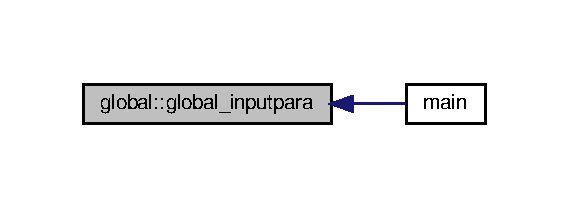
\includegraphics[width=273pt]{namespaceglobal_a930b565da2644b675f35b91735e11ce3_icgraph}
\end{center}
\end{figure}


\subsection{Variable Documentation}
\mbox{\Hypertarget{namespaceglobal_abe54a711bf9d8c30a6debfb651bdf47d}\label{namespaceglobal_abe54a711bf9d8c30a6debfb651bdf47d}} 
\index{global@{global}!alphag@{alphag}}
\index{alphag@{alphag}!global@{global}}
\subsubsection{\texorpdfstring{alphag}{alphag}}
{\footnotesize\ttfamily double precision global\+::alphag}



Thermal expansion coefficient x gravitational acceleration. 

\mbox{\Hypertarget{namespaceglobal_acf5521de662915885b6a73718cd6314b}\label{namespaceglobal_acf5521de662915885b6a73718cd6314b}} 
\index{global@{global}!ct@{ct}}
\index{ct@{ct}!global@{global}}
\subsubsection{\texorpdfstring{ct}{ct}}
{\footnotesize\ttfamily double precision global\+::ct}



Thermal diffusivity. 

\mbox{\Hypertarget{namespaceglobal_a24d27ecfb0e7d422997122c9345bac8b}\label{namespaceglobal_a24d27ecfb0e7d422997122c9345bac8b}} 
\index{global@{global}!dt@{dt}}
\index{dt@{dt}!global@{global}}
\subsubsection{\texorpdfstring{dt}{dt}}
{\footnotesize\ttfamily double precision global\+::dt}



Length of time step. 

\mbox{\Hypertarget{namespaceglobal_a3c8fbc22da61f7188e79bad2b9ba1d16}\label{namespaceglobal_a3c8fbc22da61f7188e79bad2b9ba1d16}} 
\index{global@{global}!dtstart@{dtstart}}
\index{dtstart@{dtstart}!global@{global}}
\subsubsection{\texorpdfstring{dtstart}{dtstart}}
{\footnotesize\ttfamily double precision global\+::dtstart}



Initial dt. 

\mbox{\Hypertarget{namespaceglobal_a9c5f8c3cf5f9b496608059fc13776b4c}\label{namespaceglobal_a9c5f8c3cf5f9b496608059fc13776b4c}} 
\index{global@{global}!dx@{dx}}
\index{dx@{dx}!global@{global}}
\subsubsection{\texorpdfstring{dx}{dx}}
{\footnotesize\ttfamily double precision global\+::dx}



Discretized grid lengths of the physical domain. 

\mbox{\Hypertarget{namespaceglobal_aa2d01c0b9c06af88ae13136658fc3dd9}\label{namespaceglobal_aa2d01c0b9c06af88ae13136658fc3dd9}} 
\index{global@{global}!dy@{dy}}
\index{dy@{dy}!global@{global}}
\subsubsection{\texorpdfstring{dy}{dy}}
{\footnotesize\ttfamily double precision global\+::dy}

\mbox{\Hypertarget{namespaceglobal_a4015487c561985eefa8cabc39f591540}\label{namespaceglobal_a4015487c561985eefa8cabc39f591540}} 
\index{global@{global}!dz@{dz}}
\index{dz@{dz}!global@{global}}
\subsubsection{\texorpdfstring{dz}{dz}}
{\footnotesize\ttfamily double precision global\+::dz}

\mbox{\Hypertarget{namespaceglobal_ac5d2ea39fc192fbb8354e665dc91b759}\label{namespaceglobal_ac5d2ea39fc192fbb8354e665dc91b759}} 
\index{global@{global}!lx@{lx}}
\index{lx@{lx}!global@{global}}
\subsubsection{\texorpdfstring{lx}{lx}}
{\footnotesize\ttfamily double precision global\+::lx}



Lengths of the physical domain. 

\mbox{\Hypertarget{namespaceglobal_a6a6ee40bbab9e114aa217f7d8570b924}\label{namespaceglobal_a6a6ee40bbab9e114aa217f7d8570b924}} 
\index{global@{global}!ly@{ly}}
\index{ly@{ly}!global@{global}}
\subsubsection{\texorpdfstring{ly}{ly}}
{\footnotesize\ttfamily double precision global\+::ly}

\mbox{\Hypertarget{namespaceglobal_a9d90050855b894304d8b4272c6a9ee71}\label{namespaceglobal_a9d90050855b894304d8b4272c6a9ee71}} 
\index{global@{global}!lz@{lz}}
\index{lz@{lz}!global@{global}}
\subsubsection{\texorpdfstring{lz}{lz}}
{\footnotesize\ttfamily double precision global\+::lz}

\mbox{\Hypertarget{namespaceglobal_a48babc9c7f07053917ca1392e7a7b721}\label{namespaceglobal_a48babc9c7f07053917ca1392e7a7b721}} 
\index{global@{global}!nu@{nu}}
\index{nu@{nu}!global@{global}}
\subsubsection{\texorpdfstring{nu}{nu}}
{\footnotesize\ttfamily double precision global\+::nu}



Kinematic viscosity. 

\mbox{\Hypertarget{namespaceglobal_a4ba10a6dbbcebb68e0d5e36a6c291898}\label{namespaceglobal_a4ba10a6dbbcebb68e0d5e36a6c291898}} 
\index{global@{global}!nx@{nx}}
\index{nx@{nx}!global@{global}}
\subsubsection{\texorpdfstring{nx}{nx}}
{\footnotesize\ttfamily integer global\+::nx}



Grid numbers in each direction. 

\mbox{\Hypertarget{namespaceglobal_aa37f5fe09139707ac1723302127436b1}\label{namespaceglobal_aa37f5fe09139707ac1723302127436b1}} 
\index{global@{global}!nxm@{nxm}}
\index{nxm@{nxm}!global@{global}}
\subsubsection{\texorpdfstring{nxm}{nxm}}
{\footnotesize\ttfamily integer global\+::nxm}



Grid numbers minus 1 in each direction. 

\mbox{\Hypertarget{namespaceglobal_a227001d8177d0295b61a39948436adaa}\label{namespaceglobal_a227001d8177d0295b61a39948436adaa}} 
\index{global@{global}!nxp@{nxp}}
\index{nxp@{nxp}!global@{global}}
\subsubsection{\texorpdfstring{nxp}{nxp}}
{\footnotesize\ttfamily integer global\+::nxp}



Grid numbers plus 1 in each direction. 

\mbox{\Hypertarget{namespaceglobal_a12dd7ca24c7675f31e6de07b1769991c}\label{namespaceglobal_a12dd7ca24c7675f31e6de07b1769991c}} 
\index{global@{global}!ny@{ny}}
\index{ny@{ny}!global@{global}}
\subsubsection{\texorpdfstring{ny}{ny}}
{\footnotesize\ttfamily integer global\+::ny}

\mbox{\Hypertarget{namespaceglobal_a9852876e90514ccc182c0ed0b27cdaad}\label{namespaceglobal_a9852876e90514ccc182c0ed0b27cdaad}} 
\index{global@{global}!nym@{nym}}
\index{nym@{nym}!global@{global}}
\subsubsection{\texorpdfstring{nym}{nym}}
{\footnotesize\ttfamily integer global\+::nym}

\mbox{\Hypertarget{namespaceglobal_a868bbe46b97daa7ff6c962fff16bbf2f}\label{namespaceglobal_a868bbe46b97daa7ff6c962fff16bbf2f}} 
\index{global@{global}!nyp@{nyp}}
\index{nyp@{nyp}!global@{global}}
\subsubsection{\texorpdfstring{nyp}{nyp}}
{\footnotesize\ttfamily integer global\+::nyp}

\mbox{\Hypertarget{namespaceglobal_ab8d7436a6037d4c1b7248107a2f07d76}\label{namespaceglobal_ab8d7436a6037d4c1b7248107a2f07d76}} 
\index{global@{global}!nz@{nz}}
\index{nz@{nz}!global@{global}}
\subsubsection{\texorpdfstring{nz}{nz}}
{\footnotesize\ttfamily integer global\+::nz}

\mbox{\Hypertarget{namespaceglobal_a76e27e2001870f6606e51d33a2c70f60}\label{namespaceglobal_a76e27e2001870f6606e51d33a2c70f60}} 
\index{global@{global}!nzm@{nzm}}
\index{nzm@{nzm}!global@{global}}
\subsubsection{\texorpdfstring{nzm}{nzm}}
{\footnotesize\ttfamily integer global\+::nzm}

\mbox{\Hypertarget{namespaceglobal_ab376cd7d790b630ad83ffcded3c56366}\label{namespaceglobal_ab376cd7d790b630ad83ffcded3c56366}} 
\index{global@{global}!nzp@{nzp}}
\index{nzp@{nzp}!global@{global}}
\subsubsection{\texorpdfstring{nzp}{nzp}}
{\footnotesize\ttfamily integer global\+::nzp}

\mbox{\Hypertarget{namespaceglobal_a2eeeef6cb4401e0205ced808c718dead}\label{namespaceglobal_a2eeeef6cb4401e0205ced808c718dead}} 
\index{global@{global}!pi@{pi}}
\index{pi@{pi}!global@{global}}
\subsubsection{\texorpdfstring{pi}{pi}}
{\footnotesize\ttfamily double precision, parameter global\+::pi = acos(-\/1.d0)}

\mbox{\Hypertarget{namespaceglobal_a31749f11f262d021576cd0d09bdc79c2}\label{namespaceglobal_a31749f11f262d021576cd0d09bdc79c2}} 
\index{global@{global}!pr@{pr}}
\index{pr@{pr}!global@{global}}
\subsubsection{\texorpdfstring{pr}{pr}}
{\footnotesize\ttfamily double precision global\+::pr}



Prandtl number. 

\mbox{\Hypertarget{namespaceglobal_a7b363950bb58d4e52dda12a928b2b9e2}\label{namespaceglobal_a7b363950bb58d4e52dda12a928b2b9e2}} 
\index{global@{global}!ra@{ra}}
\index{ra@{ra}!global@{global}}
\subsubsection{\texorpdfstring{ra}{ra}}
{\footnotesize\ttfamily double precision global\+::ra}



Reyleigh number. 

\mbox{\Hypertarget{namespaceglobal_a367640054e0083add94204f1a61bd61a}\label{namespaceglobal_a367640054e0083add94204f1a61bd61a}} 
\index{global@{global}!theta\+\_\+cold@{theta\+\_\+cold}}
\index{theta\+\_\+cold@{theta\+\_\+cold}!global@{global}}
\subsubsection{\texorpdfstring{theta\+\_\+cold}{theta\_cold}}
{\footnotesize\ttfamily double precision global\+::theta\+\_\+cold}



Boundary temperature of cold wall. 

\mbox{\Hypertarget{namespaceglobal_a63b846fbcd5aedd45f92a0b1eb972244}\label{namespaceglobal_a63b846fbcd5aedd45f92a0b1eb972244}} 
\index{global@{global}!theta\+\_\+hot@{theta\+\_\+hot}}
\index{theta\+\_\+hot@{theta\+\_\+hot}!global@{global}}
\subsubsection{\texorpdfstring{theta\+\_\+hot}{theta\_hot}}
{\footnotesize\ttfamily double precision global\+::theta\+\_\+hot}



Boundary temperature of hot wall. 

\mbox{\Hypertarget{namespaceglobal_a33db542cca17d8c3a156e90d31d8abe5}\label{namespaceglobal_a33db542cca17d8c3a156e90d31d8abe5}} 
\index{global@{global}!thread\+\_\+in\+\_\+x@{thread\+\_\+in\+\_\+x}}
\index{thread\+\_\+in\+\_\+x@{thread\+\_\+in\+\_\+x}!global@{global}}
\subsubsection{\texorpdfstring{thread\+\_\+in\+\_\+x}{thread\_in\_x}}
{\footnotesize\ttfamily integer global\+::thread\+\_\+in\+\_\+x}

\mbox{\Hypertarget{namespaceglobal_a0c53f9dfde5486b01023d0c9479db29c}\label{namespaceglobal_a0c53f9dfde5486b01023d0c9479db29c}} 
\index{global@{global}!thread\+\_\+in\+\_\+x\+\_\+pascal@{thread\+\_\+in\+\_\+x\+\_\+pascal}}
\index{thread\+\_\+in\+\_\+x\+\_\+pascal@{thread\+\_\+in\+\_\+x\+\_\+pascal}!global@{global}}
\subsubsection{\texorpdfstring{thread\+\_\+in\+\_\+x\+\_\+pascal}{thread\_in\_x\_pascal}}
{\footnotesize\ttfamily integer global\+::thread\+\_\+in\+\_\+x\+\_\+pascal}

\mbox{\Hypertarget{namespaceglobal_a2694e42b57b63e348f472d5a59bfe0fb}\label{namespaceglobal_a2694e42b57b63e348f472d5a59bfe0fb}} 
\index{global@{global}!thread\+\_\+in\+\_\+y@{thread\+\_\+in\+\_\+y}}
\index{thread\+\_\+in\+\_\+y@{thread\+\_\+in\+\_\+y}!global@{global}}
\subsubsection{\texorpdfstring{thread\+\_\+in\+\_\+y}{thread\_in\_y}}
{\footnotesize\ttfamily integer global\+::thread\+\_\+in\+\_\+y}

\mbox{\Hypertarget{namespaceglobal_af395b143d44c9d28517e64a695920dda}\label{namespaceglobal_af395b143d44c9d28517e64a695920dda}} 
\index{global@{global}!thread\+\_\+in\+\_\+y\+\_\+pascal@{thread\+\_\+in\+\_\+y\+\_\+pascal}}
\index{thread\+\_\+in\+\_\+y\+\_\+pascal@{thread\+\_\+in\+\_\+y\+\_\+pascal}!global@{global}}
\subsubsection{\texorpdfstring{thread\+\_\+in\+\_\+y\+\_\+pascal}{thread\_in\_y\_pascal}}
{\footnotesize\ttfamily integer global\+::thread\+\_\+in\+\_\+y\+\_\+pascal}

\mbox{\Hypertarget{namespaceglobal_a1f39f066a0ed398d1e3e56d13d092718}\label{namespaceglobal_a1f39f066a0ed398d1e3e56d13d092718}} 
\index{global@{global}!thread\+\_\+in\+\_\+z@{thread\+\_\+in\+\_\+z}}
\index{thread\+\_\+in\+\_\+z@{thread\+\_\+in\+\_\+z}!global@{global}}
\subsubsection{\texorpdfstring{thread\+\_\+in\+\_\+z}{thread\_in\_z}}
{\footnotesize\ttfamily integer global\+::thread\+\_\+in\+\_\+z}

\mbox{\Hypertarget{namespaceglobal_ac8816f9dd096716fb9b7e61d57cc5189}\label{namespaceglobal_ac8816f9dd096716fb9b7e61d57cc5189}} 
\index{global@{global}!tmax@{tmax}}
\index{tmax@{tmax}!global@{global}}
\subsubsection{\texorpdfstring{tmax}{tmax}}
{\footnotesize\ttfamily integer global\+::tmax}



Maximum number of iteration steps. 

\mbox{\Hypertarget{namespaceglobal_a07363365436fd22a91cdb5a847b4bb88}\label{namespaceglobal_a07363365436fd22a91cdb5a847b4bb88}} 
\index{global@{global}!tstart@{tstart}}
\index{tstart@{tstart}!global@{global}}
\subsubsection{\texorpdfstring{tstart}{tstart}}
{\footnotesize\ttfamily double precision global\+::tstart}



Initial simulation time. 


\hypertarget{namespacempi__subdomain}{}\section{mpi\+\_\+subdomain Module Reference}
\label{namespacempi__subdomain}\index{mpi\+\_\+subdomain@{mpi\+\_\+subdomain}}


Module for building subdomains from the physical domain.  


\subsection*{Functions/\+Subroutines}
\begin{DoxyCompactItemize}
\item 
subroutine, public \hyperlink{namespacempi__subdomain_a3a1e7cf64aafbebd3c09b92fc56bd311}{mpi\+\_\+subdomain\+\_\+make} (nprocs\+\_\+in\+\_\+x, myrank\+\_\+in\+\_\+x, nprocs\+\_\+in\+\_\+y, myrank\+\_\+in\+\_\+y, nprocs\+\_\+in\+\_\+z, myrank\+\_\+in\+\_\+z)
\begin{DoxyCompactList}\small\item\em Prepare the subdomain and determine the size of the subdomain. \end{DoxyCompactList}\item 
subroutine, public \hyperlink{namespacempi__subdomain_a56e9f2afd59e45fcada0f1c21a90eefe}{mpi\+\_\+subdomain\+\_\+clean}
\begin{DoxyCompactList}\small\item\em Deallocate subdomain variables. \end{DoxyCompactList}\item 
subroutine, public \hyperlink{namespacempi__subdomain_ad788c273d92ea7058caf0874bffdad6d}{mpi\+\_\+subdomain\+\_\+make\+\_\+ghostcell\+\_\+ddtype}
\begin{DoxyCompactList}\small\item\em Build derived datatypes for subdomain communication using ghostcells. \end{DoxyCompactList}\item 
subroutine, public \hyperlink{namespacempi__subdomain_a2e34a77537009dd448375e8fdc8d5b62}{mpi\+\_\+subdomain\+\_\+ghostcell\+\_\+update} (theta\+\_\+sub, comm\+\_\+1d\+\_\+x, comm\+\_\+1d\+\_\+y, comm\+\_\+1d\+\_\+z)
\begin{DoxyCompactList}\small\item\em Update the values of boundary ghostcells through communication in all directions. \end{DoxyCompactList}\item 
subroutine, public \hyperlink{namespacempi__subdomain_afe948dc18da021f2448cf9a6265155fe}{mpi\+\_\+subdomain\+\_\+indices} (myrank\+\_\+in\+\_\+y, nprocs\+\_\+in\+\_\+y)
\begin{DoxyCompactList}\small\item\em Determine whether the next grids are empty(0) or not(1) only in the y-\/direction. \end{DoxyCompactList}\item 
subroutine, public \hyperlink{namespacempi__subdomain_a612331eead74041f174ece9a572c7427}{mpi\+\_\+subdomain\+\_\+mesh} (myrank\+\_\+in\+\_\+x, myrank\+\_\+in\+\_\+y, myrank\+\_\+in\+\_\+z, nprocs\+\_\+in\+\_\+x, nprocs\+\_\+in\+\_\+y, nprocs\+\_\+in\+\_\+z)
\begin{DoxyCompactList}\small\item\em Assign grid coordinates and lengths of subdomains. \end{DoxyCompactList}\item 
subroutine, public \hyperlink{namespacempi__subdomain_a7cc0deb85b84358eb7addeea849733c4}{mpi\+\_\+subdomain\+\_\+initialization} (theta\+\_\+sub, myrank\+\_\+in\+\_\+y, nprocs\+\_\+in\+\_\+y)
\begin{DoxyCompactList}\small\item\em Initialize the values of the main variable in a subdomain. \end{DoxyCompactList}\item 
subroutine, public \hyperlink{namespacempi__subdomain_a55659431068678c08d21847338390ea8}{mpi\+\_\+subdomain\+\_\+boundary} (theta\+\_\+sub, myrank\+\_\+in\+\_\+y, nprocs\+\_\+in\+\_\+y)
\begin{DoxyCompactList}\small\item\em Assign the values of boundary grids in the subdomain. \end{DoxyCompactList}\end{DoxyCompactItemize}
\subsection*{Variables}
\begin{DoxyCompactItemize}
\item 
integer \hyperlink{namespacempi__subdomain_acd16f258caed20a7d8d38cd28ae64688}{ierr}
\item 
double precision, dimension(\+:,\+:), allocatable, public \hyperlink{namespacempi__subdomain_ad61f27caf5f32301a077e21363c2d73b}{thetabc3\+\_\+sub}
\begin{DoxyCompactList}\small\item\em B.\+C. of lower wall. \end{DoxyCompactList}\item 
double precision, dimension(\+:,\+:), allocatable, public \hyperlink{namespacempi__subdomain_ad1705bede0c0d39ad16f9f94afe32be6}{thetabc4\+\_\+sub}
\begin{DoxyCompactList}\small\item\em B.\+C. of upper wall. \end{DoxyCompactList}\item 
integer, dimension(\+:), allocatable, public \hyperlink{namespacempi__subdomain_ac22380b1c941dd6c53cabe7287d185e9}{jmbc\+\_\+index}
\begin{DoxyCompactList}\small\item\em Flag whether lower grid is empty(0) or not. \end{DoxyCompactList}\item 
integer, dimension(\+:), allocatable, public \hyperlink{namespacempi__subdomain_a9adbfdd11c7e9fdb968bb8eef2b13c2b}{jpbc\+\_\+index}
\begin{DoxyCompactList}\small\item\em Flag whether upper grid is empty(0) or not. \end{DoxyCompactList}\end{DoxyCompactItemize}
\textbf{ }\par
\begin{DoxyCompactItemize}
\item 
integer, public \hyperlink{namespacempi__subdomain_a005fe127fe0fc85b932814a820a36444}{nx\+\_\+sub}
\begin{DoxyCompactList}\small\item\em Grid numbers in the subdomain. \end{DoxyCompactList}\item 
integer, public \hyperlink{namespacempi__subdomain_a665ba05d0ae9309dd28b9b513a0c87a1}{ny\+\_\+sub}
\item 
integer, public \hyperlink{namespacempi__subdomain_a07555cc931ac78376a4c81207662251f}{nz\+\_\+sub}
\end{DoxyCompactItemize}

\textbf{ }\par
\begin{DoxyCompactItemize}
\item 
integer, public \hyperlink{namespacempi__subdomain_ab8925faaa6f45326c1d11efa37e03566}{ista}
\begin{DoxyCompactList}\small\item\em Grid indices of the assigned range. \end{DoxyCompactList}\item 
integer, public \hyperlink{namespacempi__subdomain_abbd7d35107c53bcfd2b2b52771f4aa67}{iend}
\item 
integer, public \hyperlink{namespacempi__subdomain_ac85bfba1caf77f9c3c0047fe9450fee6}{jsta}
\item 
integer, public \hyperlink{namespacempi__subdomain_a06433a0d1a081c51202a0010c21c9d36}{jend}
\item 
integer, public \hyperlink{namespacempi__subdomain_acd499eb1d07159aa9f5c878f9519b00f}{ksta}
\item 
integer, public \hyperlink{namespacempi__subdomain_af9934313b1ccbcb09f30916df3326076}{kend}
\end{DoxyCompactItemize}

\textbf{ }\par
\begin{DoxyCompactItemize}
\item 
double precision, dimension(\+:), allocatable, public \hyperlink{namespacempi__subdomain_a978554e1520c79471ef3793ed1872b37}{x\+\_\+sub}
\begin{DoxyCompactList}\small\item\em Coordinates of grid points in the subdomain. \end{DoxyCompactList}\item 
double precision, dimension(\+:), allocatable, public \hyperlink{namespacempi__subdomain_a58b09abee5f1002de7b20b1b86f5c821}{y\+\_\+sub}
\item 
double precision, dimension(\+:), allocatable, public \hyperlink{namespacempi__subdomain_aab6d78e49471a9a3db5ad9df4c3d4041}{z\+\_\+sub}
\end{DoxyCompactItemize}

\textbf{ }\par
\begin{DoxyCompactItemize}
\item 
double precision, dimension(\+:), allocatable, public \hyperlink{namespacempi__subdomain_a56af1740899dc9df6868e5e71a0884a5}{dmx\+\_\+sub}
\begin{DoxyCompactList}\small\item\em Grid lengths in the subdomain. \end{DoxyCompactList}\item 
double precision, dimension(\+:), allocatable, public \hyperlink{namespacempi__subdomain_ae44efbff9669bfad03a79ab41b5e8ace}{dmy\+\_\+sub}
\item 
double precision, dimension(\+:), allocatable, public \hyperlink{namespacempi__subdomain_afb6341d7362587d6fd0a06fe78ba4e3f}{dmz\+\_\+sub}
\end{DoxyCompactItemize}

\textbf{ }\par
\begin{DoxyCompactItemize}
\item 
integer \hyperlink{namespacempi__subdomain_a93395266b1630e5a91e8e89531dfcec6}{ddtype\+\_\+sendto\+\_\+e}
\begin{DoxyCompactList}\small\item\em Derived datatype for communication between x-\/neighbor subdomains. \end{DoxyCompactList}\item 
integer \hyperlink{namespacempi__subdomain_a0b2a4ab6d6a88a3817f473a5c2c172b9}{ddtype\+\_\+recvfrom\+\_\+w}
\item 
integer \hyperlink{namespacempi__subdomain_a0701fde01daea1a6fd51b62c75b8ee82}{ddtype\+\_\+sendto\+\_\+w}
\item 
integer \hyperlink{namespacempi__subdomain_a18a84c0f3ca27cd4dd73057ff035f341}{ddtype\+\_\+recvfrom\+\_\+e}
\end{DoxyCompactItemize}

\textbf{ }\par
\begin{DoxyCompactItemize}
\item 
integer \hyperlink{namespacempi__subdomain_a55f5c1af9bd941fd176e619bddbb8d82}{ddtype\+\_\+sendto\+\_\+n}
\begin{DoxyCompactList}\small\item\em Derived datatype for communication between y-\/neighbor subdomains. \end{DoxyCompactList}\item 
integer \hyperlink{namespacempi__subdomain_a1f46916f08758533cad3ecac33233e38}{ddtype\+\_\+recvfrom\+\_\+s}
\item 
integer \hyperlink{namespacempi__subdomain_a660f83d621188fb7eb60ad10eab4c9b5}{ddtype\+\_\+sendto\+\_\+s}
\item 
integer \hyperlink{namespacempi__subdomain_a74f1edb3c9227692b250285680518dc4}{ddtype\+\_\+recvfrom\+\_\+n}
\end{DoxyCompactItemize}

\textbf{ }\par
\begin{DoxyCompactItemize}
\item 
integer \hyperlink{namespacempi__subdomain_a4f3d66535b947c7afee75e6e73a47206}{ddtype\+\_\+sendto\+\_\+f}
\begin{DoxyCompactList}\small\item\em Derived datatype for communication between z-\/neighbor subdomains. \end{DoxyCompactList}\item 
integer \hyperlink{namespacempi__subdomain_ad6462f18c8c68c076005957e9d062252}{ddtype\+\_\+recvfrom\+\_\+b}
\item 
integer \hyperlink{namespacempi__subdomain_a7a2af0322a7aaa435951a5432859687a}{ddtype\+\_\+sendto\+\_\+b}
\item 
integer \hyperlink{namespacempi__subdomain_a4da19838e8bc3934ad5c24db424bec2c}{ddtype\+\_\+recvfrom\+\_\+f}
\end{DoxyCompactItemize}



\subsection{Detailed Description}
Module for building subdomains from the physical domain. 

This module has simulation parameters for subdomains and communication between the subdomains. 

\subsection{Function/\+Subroutine Documentation}
\mbox{\Hypertarget{namespacempi__subdomain_a55659431068678c08d21847338390ea8}\label{namespacempi__subdomain_a55659431068678c08d21847338390ea8}} 
\index{mpi\+\_\+subdomain@{mpi\+\_\+subdomain}!mpi\+\_\+subdomain\+\_\+boundary@{mpi\+\_\+subdomain\+\_\+boundary}}
\index{mpi\+\_\+subdomain\+\_\+boundary@{mpi\+\_\+subdomain\+\_\+boundary}!mpi\+\_\+subdomain@{mpi\+\_\+subdomain}}
\subsubsection{\texorpdfstring{mpi\+\_\+subdomain\+\_\+boundary()}{mpi\_subdomain\_boundary()}}
{\footnotesize\ttfamily subroutine, public mpi\+\_\+subdomain\+::mpi\+\_\+subdomain\+\_\+boundary (\begin{DoxyParamCaption}\item[{double precision, dimension(0\+:\hyperlink{namespacempi__subdomain_a005fe127fe0fc85b932814a820a36444}{nx\+\_\+sub}, 0\+:\hyperlink{namespacempi__subdomain_a665ba05d0ae9309dd28b9b513a0c87a1}{ny\+\_\+sub}, 0\+:\hyperlink{namespacempi__subdomain_a07555cc931ac78376a4c81207662251f}{nz\+\_\+sub}), intent(in)}]{theta\+\_\+sub,  }\item[{integer, intent(in)}]{myrank\+\_\+in\+\_\+y,  }\item[{integer, intent(in)}]{nprocs\+\_\+in\+\_\+y }\end{DoxyParamCaption})}



Assign the values of boundary grids in the subdomain. 


\begin{DoxyParams}{Parameters}
{\em theta\+\_\+sub} & Main variable to be solved \\
\hline
{\em myrank\+\_\+in\+\_\+y} & Rank ID in y-\/direction \\
\hline
{\em nprocs\+\_\+in\+\_\+y} & Number of M\+PI processes in y-\/direction \\
\hline
\end{DoxyParams}
Here is the caller graph for this function\+:
\nopagebreak
\begin{figure}[H]
\begin{center}
\leavevmode
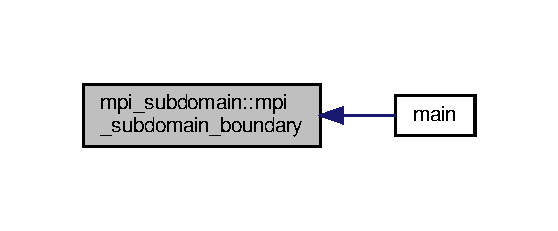
\includegraphics[width=268pt]{namespacempi__subdomain_a55659431068678c08d21847338390ea8_icgraph}
\end{center}
\end{figure}
\mbox{\Hypertarget{namespacempi__subdomain_a56e9f2afd59e45fcada0f1c21a90eefe}\label{namespacempi__subdomain_a56e9f2afd59e45fcada0f1c21a90eefe}} 
\index{mpi\+\_\+subdomain@{mpi\+\_\+subdomain}!mpi\+\_\+subdomain\+\_\+clean@{mpi\+\_\+subdomain\+\_\+clean}}
\index{mpi\+\_\+subdomain\+\_\+clean@{mpi\+\_\+subdomain\+\_\+clean}!mpi\+\_\+subdomain@{mpi\+\_\+subdomain}}
\subsubsection{\texorpdfstring{mpi\+\_\+subdomain\+\_\+clean()}{mpi\_subdomain\_clean()}}
{\footnotesize\ttfamily subroutine, public mpi\+\_\+subdomain\+::mpi\+\_\+subdomain\+\_\+clean (\begin{DoxyParamCaption}{ }\end{DoxyParamCaption})}



Deallocate subdomain variables. 

Here is the caller graph for this function\+:
\nopagebreak
\begin{figure}[H]
\begin{center}
\leavevmode
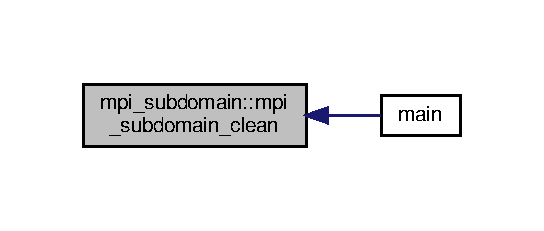
\includegraphics[width=261pt]{namespacempi__subdomain_a56e9f2afd59e45fcada0f1c21a90eefe_icgraph}
\end{center}
\end{figure}
\mbox{\Hypertarget{namespacempi__subdomain_a2e34a77537009dd448375e8fdc8d5b62}\label{namespacempi__subdomain_a2e34a77537009dd448375e8fdc8d5b62}} 
\index{mpi\+\_\+subdomain@{mpi\+\_\+subdomain}!mpi\+\_\+subdomain\+\_\+ghostcell\+\_\+update@{mpi\+\_\+subdomain\+\_\+ghostcell\+\_\+update}}
\index{mpi\+\_\+subdomain\+\_\+ghostcell\+\_\+update@{mpi\+\_\+subdomain\+\_\+ghostcell\+\_\+update}!mpi\+\_\+subdomain@{mpi\+\_\+subdomain}}
\subsubsection{\texorpdfstring{mpi\+\_\+subdomain\+\_\+ghostcell\+\_\+update()}{mpi\_subdomain\_ghostcell\_update()}}
{\footnotesize\ttfamily subroutine, public mpi\+\_\+subdomain\+::mpi\+\_\+subdomain\+\_\+ghostcell\+\_\+update (\begin{DoxyParamCaption}\item[{double precision, dimension(0\+:\hyperlink{namespacempi__subdomain_a005fe127fe0fc85b932814a820a36444}{nx\+\_\+sub}, 0\+:\hyperlink{namespacempi__subdomain_a665ba05d0ae9309dd28b9b513a0c87a1}{ny\+\_\+sub}, 0\+:\hyperlink{namespacempi__subdomain_a07555cc931ac78376a4c81207662251f}{nz\+\_\+sub}), intent(inout)}]{theta\+\_\+sub,  }\item[{type(\hyperlink{structmpi__topology_1_1cart__comm__1d}{cart\+\_\+comm\+\_\+1d}), intent(in)}]{comm\+\_\+1d\+\_\+x,  }\item[{type(\hyperlink{structmpi__topology_1_1cart__comm__1d}{cart\+\_\+comm\+\_\+1d}), intent(in)}]{comm\+\_\+1d\+\_\+y,  }\item[{type(\hyperlink{structmpi__topology_1_1cart__comm__1d}{cart\+\_\+comm\+\_\+1d}), intent(in)}]{comm\+\_\+1d\+\_\+z }\end{DoxyParamCaption})}



Update the values of boundary ghostcells through communication in all directions. 


\begin{DoxyParams}{Parameters}
{\em theta\+\_\+sub} & Variables to be updated \\
\hline
{\em comm\+\_\+1d\+\_\+x} & Subcommunicator in the x-\/direction \\
\hline
{\em comm\+\_\+1d\+\_\+y} & Subcommunicator in the y-\/direction \\
\hline
{\em comm\+\_\+1d\+\_\+z} & Subcommunicator in the z-\/direction \\
\hline
\end{DoxyParams}
Here is the caller graph for this function\+:
\nopagebreak
\begin{figure}[H]
\begin{center}
\leavevmode
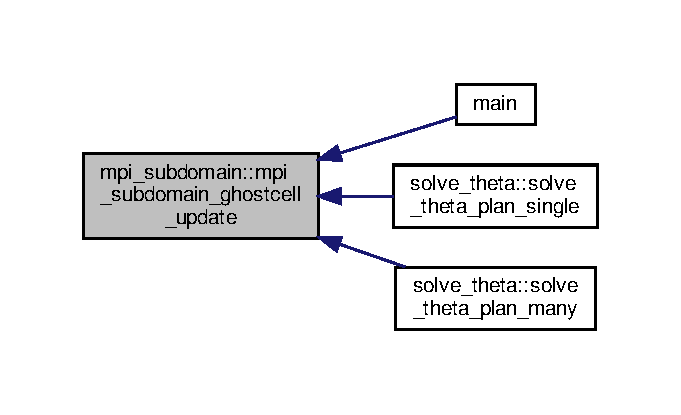
\includegraphics[width=327pt]{namespacempi__subdomain_a2e34a77537009dd448375e8fdc8d5b62_icgraph}
\end{center}
\end{figure}
\mbox{\Hypertarget{namespacempi__subdomain_afe948dc18da021f2448cf9a6265155fe}\label{namespacempi__subdomain_afe948dc18da021f2448cf9a6265155fe}} 
\index{mpi\+\_\+subdomain@{mpi\+\_\+subdomain}!mpi\+\_\+subdomain\+\_\+indices@{mpi\+\_\+subdomain\+\_\+indices}}
\index{mpi\+\_\+subdomain\+\_\+indices@{mpi\+\_\+subdomain\+\_\+indices}!mpi\+\_\+subdomain@{mpi\+\_\+subdomain}}
\subsubsection{\texorpdfstring{mpi\+\_\+subdomain\+\_\+indices()}{mpi\_subdomain\_indices()}}
{\footnotesize\ttfamily subroutine, public mpi\+\_\+subdomain\+::mpi\+\_\+subdomain\+\_\+indices (\begin{DoxyParamCaption}\item[{integer, intent(in)}]{myrank\+\_\+in\+\_\+y,  }\item[{integer, intent(in)}]{nprocs\+\_\+in\+\_\+y }\end{DoxyParamCaption})}



Determine whether the next grids are empty(0) or not(1) only in the y-\/direction. 


\begin{DoxyParams}{Parameters}
{\em nprocs\+\_\+in\+\_\+y} & Number of M\+PI processes in y-\/direction \\
\hline
{\em myrank\+\_\+in\+\_\+y} & Rank ID in y-\/direction \\
\hline
\end{DoxyParams}
Here is the caller graph for this function\+:
\nopagebreak
\begin{figure}[H]
\begin{center}
\leavevmode
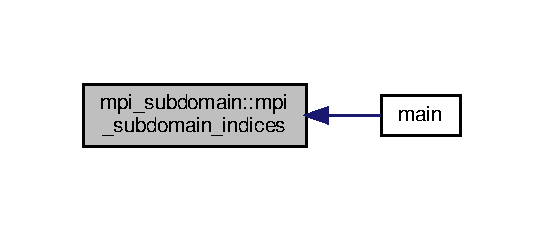
\includegraphics[width=261pt]{namespacempi__subdomain_afe948dc18da021f2448cf9a6265155fe_icgraph}
\end{center}
\end{figure}
\mbox{\Hypertarget{namespacempi__subdomain_a7cc0deb85b84358eb7addeea849733c4}\label{namespacempi__subdomain_a7cc0deb85b84358eb7addeea849733c4}} 
\index{mpi\+\_\+subdomain@{mpi\+\_\+subdomain}!mpi\+\_\+subdomain\+\_\+initialization@{mpi\+\_\+subdomain\+\_\+initialization}}
\index{mpi\+\_\+subdomain\+\_\+initialization@{mpi\+\_\+subdomain\+\_\+initialization}!mpi\+\_\+subdomain@{mpi\+\_\+subdomain}}
\subsubsection{\texorpdfstring{mpi\+\_\+subdomain\+\_\+initialization()}{mpi\_subdomain\_initialization()}}
{\footnotesize\ttfamily subroutine, public mpi\+\_\+subdomain\+::mpi\+\_\+subdomain\+\_\+initialization (\begin{DoxyParamCaption}\item[{double precision, dimension(0\+:\hyperlink{namespacempi__subdomain_a005fe127fe0fc85b932814a820a36444}{nx\+\_\+sub}, 0\+:\hyperlink{namespacempi__subdomain_a665ba05d0ae9309dd28b9b513a0c87a1}{ny\+\_\+sub}, 0\+:\hyperlink{namespacempi__subdomain_a07555cc931ac78376a4c81207662251f}{nz\+\_\+sub}), intent(inout)}]{theta\+\_\+sub,  }\item[{integer, intent(in)}]{myrank\+\_\+in\+\_\+y,  }\item[{integer, intent(in)}]{nprocs\+\_\+in\+\_\+y }\end{DoxyParamCaption})}



Initialize the values of the main variable in a subdomain. 


\begin{DoxyParams}{Parameters}
{\em theta\+\_\+sub} & Main variable to be solved \\
\hline
{\em myrank\+\_\+in\+\_\+y} & Rank ID in y-\/direction \\
\hline
{\em nprocs\+\_\+in\+\_\+y} & Number of M\+PI processes in y-\/direction \\
\hline
\end{DoxyParams}
Here is the caller graph for this function\+:
\nopagebreak
\begin{figure}[H]
\begin{center}
\leavevmode
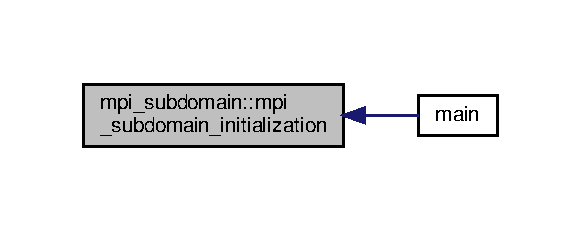
\includegraphics[width=279pt]{namespacempi__subdomain_a7cc0deb85b84358eb7addeea849733c4_icgraph}
\end{center}
\end{figure}
\mbox{\Hypertarget{namespacempi__subdomain_a3a1e7cf64aafbebd3c09b92fc56bd311}\label{namespacempi__subdomain_a3a1e7cf64aafbebd3c09b92fc56bd311}} 
\index{mpi\+\_\+subdomain@{mpi\+\_\+subdomain}!mpi\+\_\+subdomain\+\_\+make@{mpi\+\_\+subdomain\+\_\+make}}
\index{mpi\+\_\+subdomain\+\_\+make@{mpi\+\_\+subdomain\+\_\+make}!mpi\+\_\+subdomain@{mpi\+\_\+subdomain}}
\subsubsection{\texorpdfstring{mpi\+\_\+subdomain\+\_\+make()}{mpi\_subdomain\_make()}}
{\footnotesize\ttfamily subroutine, public mpi\+\_\+subdomain\+::mpi\+\_\+subdomain\+\_\+make (\begin{DoxyParamCaption}\item[{integer, intent(in)}]{nprocs\+\_\+in\+\_\+x,  }\item[{integer, intent(in)}]{myrank\+\_\+in\+\_\+x,  }\item[{integer, intent(in)}]{nprocs\+\_\+in\+\_\+y,  }\item[{integer, intent(in)}]{myrank\+\_\+in\+\_\+y,  }\item[{integer, intent(in)}]{nprocs\+\_\+in\+\_\+z,  }\item[{integer, intent(in)}]{myrank\+\_\+in\+\_\+z }\end{DoxyParamCaption})}



Prepare the subdomain and determine the size of the subdomain. 


\begin{DoxyParams}{Parameters}
{\em nprocs\+\_\+in\+\_\+x} & Number of M\+PI processes in x-\/direction \\
\hline
{\em myrank\+\_\+in\+\_\+x} & Rank ID in x-\/direction \\
\hline
{\em nprocs\+\_\+in\+\_\+y} & Number of M\+PI processes in y-\/direction \\
\hline
{\em myrank\+\_\+in\+\_\+y} & Rank ID in y-\/direction \\
\hline
{\em nprocs\+\_\+in\+\_\+z} & Number of M\+PI processes in z-\/direction \\
\hline
{\em myrank\+\_\+in\+\_\+z} & Rank ID in z-\/direction \\
\hline
\end{DoxyParams}
Here is the call graph for this function\+:
\nopagebreak
\begin{figure}[H]
\begin{center}
\leavevmode
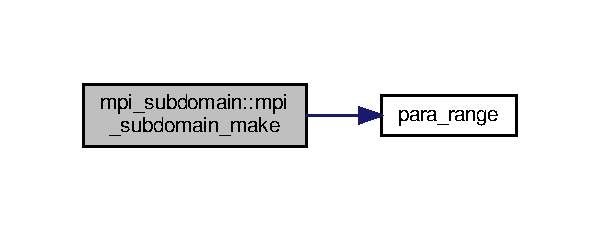
\includegraphics[width=288pt]{namespacempi__subdomain_a3a1e7cf64aafbebd3c09b92fc56bd311_cgraph}
\end{center}
\end{figure}
Here is the caller graph for this function\+:
\nopagebreak
\begin{figure}[H]
\begin{center}
\leavevmode
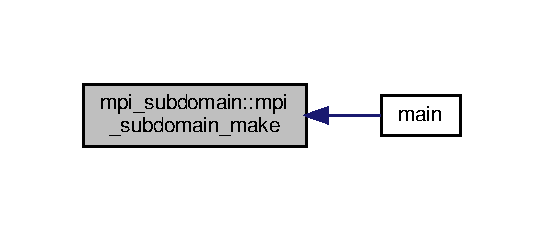
\includegraphics[width=261pt]{namespacempi__subdomain_a3a1e7cf64aafbebd3c09b92fc56bd311_icgraph}
\end{center}
\end{figure}
\mbox{\Hypertarget{namespacempi__subdomain_ad788c273d92ea7058caf0874bffdad6d}\label{namespacempi__subdomain_ad788c273d92ea7058caf0874bffdad6d}} 
\index{mpi\+\_\+subdomain@{mpi\+\_\+subdomain}!mpi\+\_\+subdomain\+\_\+make\+\_\+ghostcell\+\_\+ddtype@{mpi\+\_\+subdomain\+\_\+make\+\_\+ghostcell\+\_\+ddtype}}
\index{mpi\+\_\+subdomain\+\_\+make\+\_\+ghostcell\+\_\+ddtype@{mpi\+\_\+subdomain\+\_\+make\+\_\+ghostcell\+\_\+ddtype}!mpi\+\_\+subdomain@{mpi\+\_\+subdomain}}
\subsubsection{\texorpdfstring{mpi\+\_\+subdomain\+\_\+make\+\_\+ghostcell\+\_\+ddtype()}{mpi\_subdomain\_make\_ghostcell\_ddtype()}}
{\footnotesize\ttfamily subroutine, public mpi\+\_\+subdomain\+::mpi\+\_\+subdomain\+\_\+make\+\_\+ghostcell\+\_\+ddtype (\begin{DoxyParamCaption}{ }\end{DoxyParamCaption})}



Build derived datatypes for subdomain communication using ghostcells. 

Here is the caller graph for this function\+:
\nopagebreak
\begin{figure}[H]
\begin{center}
\leavevmode
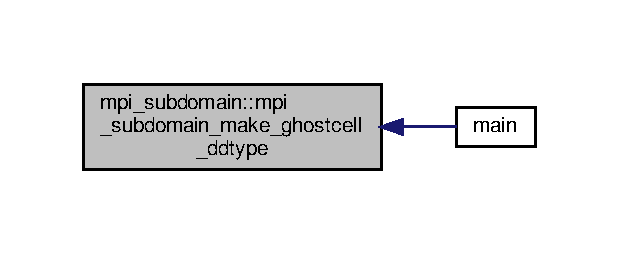
\includegraphics[width=297pt]{namespacempi__subdomain_ad788c273d92ea7058caf0874bffdad6d_icgraph}
\end{center}
\end{figure}
\mbox{\Hypertarget{namespacempi__subdomain_a612331eead74041f174ece9a572c7427}\label{namespacempi__subdomain_a612331eead74041f174ece9a572c7427}} 
\index{mpi\+\_\+subdomain@{mpi\+\_\+subdomain}!mpi\+\_\+subdomain\+\_\+mesh@{mpi\+\_\+subdomain\+\_\+mesh}}
\index{mpi\+\_\+subdomain\+\_\+mesh@{mpi\+\_\+subdomain\+\_\+mesh}!mpi\+\_\+subdomain@{mpi\+\_\+subdomain}}
\subsubsection{\texorpdfstring{mpi\+\_\+subdomain\+\_\+mesh()}{mpi\_subdomain\_mesh()}}
{\footnotesize\ttfamily subroutine, public mpi\+\_\+subdomain\+::mpi\+\_\+subdomain\+\_\+mesh (\begin{DoxyParamCaption}\item[{integer, intent(in)}]{myrank\+\_\+in\+\_\+x,  }\item[{integer, intent(in)}]{myrank\+\_\+in\+\_\+y,  }\item[{integer, intent(in)}]{myrank\+\_\+in\+\_\+z,  }\item[{integer, intent(in)}]{nprocs\+\_\+in\+\_\+x,  }\item[{integer, intent(in)}]{nprocs\+\_\+in\+\_\+y,  }\item[{integer, intent(in)}]{nprocs\+\_\+in\+\_\+z }\end{DoxyParamCaption})}



Assign grid coordinates and lengths of subdomains. 


\begin{DoxyParams}{Parameters}
{\em myrank\+\_\+in\+\_\+x} & Rank ID in x-\/direction \\
\hline
{\em myrank\+\_\+in\+\_\+y} & Rank ID in y-\/direction \\
\hline
{\em myrank\+\_\+in\+\_\+z} & Rank ID in z-\/direction \\
\hline
{\em nprocs\+\_\+in\+\_\+x} & Number of M\+PI processes in x-\/direction \\
\hline
{\em nprocs\+\_\+in\+\_\+y} & Number of M\+PI processes in y-\/direction \\
\hline
{\em nprocs\+\_\+in\+\_\+z} & Number of M\+PI processes in z-\/direction \\
\hline
\end{DoxyParams}
Here is the caller graph for this function\+:
\nopagebreak
\begin{figure}[H]
\begin{center}
\leavevmode
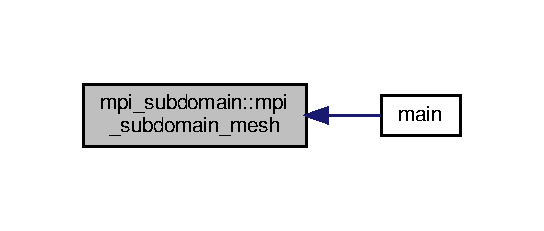
\includegraphics[width=261pt]{namespacempi__subdomain_a612331eead74041f174ece9a572c7427_icgraph}
\end{center}
\end{figure}


\subsection{Variable Documentation}
\mbox{\Hypertarget{namespacempi__subdomain_ad6462f18c8c68c076005957e9d062252}\label{namespacempi__subdomain_ad6462f18c8c68c076005957e9d062252}} 
\index{mpi\+\_\+subdomain@{mpi\+\_\+subdomain}!ddtype\+\_\+recvfrom\+\_\+b@{ddtype\+\_\+recvfrom\+\_\+b}}
\index{ddtype\+\_\+recvfrom\+\_\+b@{ddtype\+\_\+recvfrom\+\_\+b}!mpi\+\_\+subdomain@{mpi\+\_\+subdomain}}
\subsubsection{\texorpdfstring{ddtype\+\_\+recvfrom\+\_\+b}{ddtype\_recvfrom\_b}}
{\footnotesize\ttfamily integer mpi\+\_\+subdomain\+::ddtype\+\_\+recvfrom\+\_\+b}

\mbox{\Hypertarget{namespacempi__subdomain_a18a84c0f3ca27cd4dd73057ff035f341}\label{namespacempi__subdomain_a18a84c0f3ca27cd4dd73057ff035f341}} 
\index{mpi\+\_\+subdomain@{mpi\+\_\+subdomain}!ddtype\+\_\+recvfrom\+\_\+e@{ddtype\+\_\+recvfrom\+\_\+e}}
\index{ddtype\+\_\+recvfrom\+\_\+e@{ddtype\+\_\+recvfrom\+\_\+e}!mpi\+\_\+subdomain@{mpi\+\_\+subdomain}}
\subsubsection{\texorpdfstring{ddtype\+\_\+recvfrom\+\_\+e}{ddtype\_recvfrom\_e}}
{\footnotesize\ttfamily integer mpi\+\_\+subdomain\+::ddtype\+\_\+recvfrom\+\_\+e}

\mbox{\Hypertarget{namespacempi__subdomain_a4da19838e8bc3934ad5c24db424bec2c}\label{namespacempi__subdomain_a4da19838e8bc3934ad5c24db424bec2c}} 
\index{mpi\+\_\+subdomain@{mpi\+\_\+subdomain}!ddtype\+\_\+recvfrom\+\_\+f@{ddtype\+\_\+recvfrom\+\_\+f}}
\index{ddtype\+\_\+recvfrom\+\_\+f@{ddtype\+\_\+recvfrom\+\_\+f}!mpi\+\_\+subdomain@{mpi\+\_\+subdomain}}
\subsubsection{\texorpdfstring{ddtype\+\_\+recvfrom\+\_\+f}{ddtype\_recvfrom\_f}}
{\footnotesize\ttfamily integer mpi\+\_\+subdomain\+::ddtype\+\_\+recvfrom\+\_\+f}

\mbox{\Hypertarget{namespacempi__subdomain_a74f1edb3c9227692b250285680518dc4}\label{namespacempi__subdomain_a74f1edb3c9227692b250285680518dc4}} 
\index{mpi\+\_\+subdomain@{mpi\+\_\+subdomain}!ddtype\+\_\+recvfrom\+\_\+n@{ddtype\+\_\+recvfrom\+\_\+n}}
\index{ddtype\+\_\+recvfrom\+\_\+n@{ddtype\+\_\+recvfrom\+\_\+n}!mpi\+\_\+subdomain@{mpi\+\_\+subdomain}}
\subsubsection{\texorpdfstring{ddtype\+\_\+recvfrom\+\_\+n}{ddtype\_recvfrom\_n}}
{\footnotesize\ttfamily integer mpi\+\_\+subdomain\+::ddtype\+\_\+recvfrom\+\_\+n}

\mbox{\Hypertarget{namespacempi__subdomain_a1f46916f08758533cad3ecac33233e38}\label{namespacempi__subdomain_a1f46916f08758533cad3ecac33233e38}} 
\index{mpi\+\_\+subdomain@{mpi\+\_\+subdomain}!ddtype\+\_\+recvfrom\+\_\+s@{ddtype\+\_\+recvfrom\+\_\+s}}
\index{ddtype\+\_\+recvfrom\+\_\+s@{ddtype\+\_\+recvfrom\+\_\+s}!mpi\+\_\+subdomain@{mpi\+\_\+subdomain}}
\subsubsection{\texorpdfstring{ddtype\+\_\+recvfrom\+\_\+s}{ddtype\_recvfrom\_s}}
{\footnotesize\ttfamily integer mpi\+\_\+subdomain\+::ddtype\+\_\+recvfrom\+\_\+s}

\mbox{\Hypertarget{namespacempi__subdomain_a0b2a4ab6d6a88a3817f473a5c2c172b9}\label{namespacempi__subdomain_a0b2a4ab6d6a88a3817f473a5c2c172b9}} 
\index{mpi\+\_\+subdomain@{mpi\+\_\+subdomain}!ddtype\+\_\+recvfrom\+\_\+w@{ddtype\+\_\+recvfrom\+\_\+w}}
\index{ddtype\+\_\+recvfrom\+\_\+w@{ddtype\+\_\+recvfrom\+\_\+w}!mpi\+\_\+subdomain@{mpi\+\_\+subdomain}}
\subsubsection{\texorpdfstring{ddtype\+\_\+recvfrom\+\_\+w}{ddtype\_recvfrom\_w}}
{\footnotesize\ttfamily integer mpi\+\_\+subdomain\+::ddtype\+\_\+recvfrom\+\_\+w}

\mbox{\Hypertarget{namespacempi__subdomain_a7a2af0322a7aaa435951a5432859687a}\label{namespacempi__subdomain_a7a2af0322a7aaa435951a5432859687a}} 
\index{mpi\+\_\+subdomain@{mpi\+\_\+subdomain}!ddtype\+\_\+sendto\+\_\+b@{ddtype\+\_\+sendto\+\_\+b}}
\index{ddtype\+\_\+sendto\+\_\+b@{ddtype\+\_\+sendto\+\_\+b}!mpi\+\_\+subdomain@{mpi\+\_\+subdomain}}
\subsubsection{\texorpdfstring{ddtype\+\_\+sendto\+\_\+b}{ddtype\_sendto\_b}}
{\footnotesize\ttfamily integer mpi\+\_\+subdomain\+::ddtype\+\_\+sendto\+\_\+b}

\mbox{\Hypertarget{namespacempi__subdomain_a93395266b1630e5a91e8e89531dfcec6}\label{namespacempi__subdomain_a93395266b1630e5a91e8e89531dfcec6}} 
\index{mpi\+\_\+subdomain@{mpi\+\_\+subdomain}!ddtype\+\_\+sendto\+\_\+e@{ddtype\+\_\+sendto\+\_\+e}}
\index{ddtype\+\_\+sendto\+\_\+e@{ddtype\+\_\+sendto\+\_\+e}!mpi\+\_\+subdomain@{mpi\+\_\+subdomain}}
\subsubsection{\texorpdfstring{ddtype\+\_\+sendto\+\_\+e}{ddtype\_sendto\_e}}
{\footnotesize\ttfamily integer mpi\+\_\+subdomain\+::ddtype\+\_\+sendto\+\_\+e}



Derived datatype for communication between x-\/neighbor subdomains. 

\mbox{\Hypertarget{namespacempi__subdomain_a4f3d66535b947c7afee75e6e73a47206}\label{namespacempi__subdomain_a4f3d66535b947c7afee75e6e73a47206}} 
\index{mpi\+\_\+subdomain@{mpi\+\_\+subdomain}!ddtype\+\_\+sendto\+\_\+f@{ddtype\+\_\+sendto\+\_\+f}}
\index{ddtype\+\_\+sendto\+\_\+f@{ddtype\+\_\+sendto\+\_\+f}!mpi\+\_\+subdomain@{mpi\+\_\+subdomain}}
\subsubsection{\texorpdfstring{ddtype\+\_\+sendto\+\_\+f}{ddtype\_sendto\_f}}
{\footnotesize\ttfamily integer mpi\+\_\+subdomain\+::ddtype\+\_\+sendto\+\_\+f}



Derived datatype for communication between z-\/neighbor subdomains. 

\mbox{\Hypertarget{namespacempi__subdomain_a55f5c1af9bd941fd176e619bddbb8d82}\label{namespacempi__subdomain_a55f5c1af9bd941fd176e619bddbb8d82}} 
\index{mpi\+\_\+subdomain@{mpi\+\_\+subdomain}!ddtype\+\_\+sendto\+\_\+n@{ddtype\+\_\+sendto\+\_\+n}}
\index{ddtype\+\_\+sendto\+\_\+n@{ddtype\+\_\+sendto\+\_\+n}!mpi\+\_\+subdomain@{mpi\+\_\+subdomain}}
\subsubsection{\texorpdfstring{ddtype\+\_\+sendto\+\_\+n}{ddtype\_sendto\_n}}
{\footnotesize\ttfamily integer mpi\+\_\+subdomain\+::ddtype\+\_\+sendto\+\_\+n}



Derived datatype for communication between y-\/neighbor subdomains. 

\mbox{\Hypertarget{namespacempi__subdomain_a660f83d621188fb7eb60ad10eab4c9b5}\label{namespacempi__subdomain_a660f83d621188fb7eb60ad10eab4c9b5}} 
\index{mpi\+\_\+subdomain@{mpi\+\_\+subdomain}!ddtype\+\_\+sendto\+\_\+s@{ddtype\+\_\+sendto\+\_\+s}}
\index{ddtype\+\_\+sendto\+\_\+s@{ddtype\+\_\+sendto\+\_\+s}!mpi\+\_\+subdomain@{mpi\+\_\+subdomain}}
\subsubsection{\texorpdfstring{ddtype\+\_\+sendto\+\_\+s}{ddtype\_sendto\_s}}
{\footnotesize\ttfamily integer mpi\+\_\+subdomain\+::ddtype\+\_\+sendto\+\_\+s}

\mbox{\Hypertarget{namespacempi__subdomain_a0701fde01daea1a6fd51b62c75b8ee82}\label{namespacempi__subdomain_a0701fde01daea1a6fd51b62c75b8ee82}} 
\index{mpi\+\_\+subdomain@{mpi\+\_\+subdomain}!ddtype\+\_\+sendto\+\_\+w@{ddtype\+\_\+sendto\+\_\+w}}
\index{ddtype\+\_\+sendto\+\_\+w@{ddtype\+\_\+sendto\+\_\+w}!mpi\+\_\+subdomain@{mpi\+\_\+subdomain}}
\subsubsection{\texorpdfstring{ddtype\+\_\+sendto\+\_\+w}{ddtype\_sendto\_w}}
{\footnotesize\ttfamily integer mpi\+\_\+subdomain\+::ddtype\+\_\+sendto\+\_\+w}

\mbox{\Hypertarget{namespacempi__subdomain_a56af1740899dc9df6868e5e71a0884a5}\label{namespacempi__subdomain_a56af1740899dc9df6868e5e71a0884a5}} 
\index{mpi\+\_\+subdomain@{mpi\+\_\+subdomain}!dmx\+\_\+sub@{dmx\+\_\+sub}}
\index{dmx\+\_\+sub@{dmx\+\_\+sub}!mpi\+\_\+subdomain@{mpi\+\_\+subdomain}}
\subsubsection{\texorpdfstring{dmx\+\_\+sub}{dmx\_sub}}
{\footnotesize\ttfamily double precision, dimension(\+:), allocatable, public mpi\+\_\+subdomain\+::dmx\+\_\+sub}



Grid lengths in the subdomain. 

\mbox{\Hypertarget{namespacempi__subdomain_ae44efbff9669bfad03a79ab41b5e8ace}\label{namespacempi__subdomain_ae44efbff9669bfad03a79ab41b5e8ace}} 
\index{mpi\+\_\+subdomain@{mpi\+\_\+subdomain}!dmy\+\_\+sub@{dmy\+\_\+sub}}
\index{dmy\+\_\+sub@{dmy\+\_\+sub}!mpi\+\_\+subdomain@{mpi\+\_\+subdomain}}
\subsubsection{\texorpdfstring{dmy\+\_\+sub}{dmy\_sub}}
{\footnotesize\ttfamily double precision, dimension(\+:), allocatable, public mpi\+\_\+subdomain\+::dmy\+\_\+sub}

\mbox{\Hypertarget{namespacempi__subdomain_afb6341d7362587d6fd0a06fe78ba4e3f}\label{namespacempi__subdomain_afb6341d7362587d6fd0a06fe78ba4e3f}} 
\index{mpi\+\_\+subdomain@{mpi\+\_\+subdomain}!dmz\+\_\+sub@{dmz\+\_\+sub}}
\index{dmz\+\_\+sub@{dmz\+\_\+sub}!mpi\+\_\+subdomain@{mpi\+\_\+subdomain}}
\subsubsection{\texorpdfstring{dmz\+\_\+sub}{dmz\_sub}}
{\footnotesize\ttfamily double precision, dimension(\+:), allocatable, public mpi\+\_\+subdomain\+::dmz\+\_\+sub}

\mbox{\Hypertarget{namespacempi__subdomain_abbd7d35107c53bcfd2b2b52771f4aa67}\label{namespacempi__subdomain_abbd7d35107c53bcfd2b2b52771f4aa67}} 
\index{mpi\+\_\+subdomain@{mpi\+\_\+subdomain}!iend@{iend}}
\index{iend@{iend}!mpi\+\_\+subdomain@{mpi\+\_\+subdomain}}
\subsubsection{\texorpdfstring{iend}{iend}}
{\footnotesize\ttfamily integer, public mpi\+\_\+subdomain\+::iend}

\mbox{\Hypertarget{namespacempi__subdomain_acd16f258caed20a7d8d38cd28ae64688}\label{namespacempi__subdomain_acd16f258caed20a7d8d38cd28ae64688}} 
\index{mpi\+\_\+subdomain@{mpi\+\_\+subdomain}!ierr@{ierr}}
\index{ierr@{ierr}!mpi\+\_\+subdomain@{mpi\+\_\+subdomain}}
\subsubsection{\texorpdfstring{ierr}{ierr}}
{\footnotesize\ttfamily integer mpi\+\_\+subdomain\+::ierr}

\mbox{\Hypertarget{namespacempi__subdomain_ab8925faaa6f45326c1d11efa37e03566}\label{namespacempi__subdomain_ab8925faaa6f45326c1d11efa37e03566}} 
\index{mpi\+\_\+subdomain@{mpi\+\_\+subdomain}!ista@{ista}}
\index{ista@{ista}!mpi\+\_\+subdomain@{mpi\+\_\+subdomain}}
\subsubsection{\texorpdfstring{ista}{ista}}
{\footnotesize\ttfamily integer, public mpi\+\_\+subdomain\+::ista}



Grid indices of the assigned range. 

\mbox{\Hypertarget{namespacempi__subdomain_a06433a0d1a081c51202a0010c21c9d36}\label{namespacempi__subdomain_a06433a0d1a081c51202a0010c21c9d36}} 
\index{mpi\+\_\+subdomain@{mpi\+\_\+subdomain}!jend@{jend}}
\index{jend@{jend}!mpi\+\_\+subdomain@{mpi\+\_\+subdomain}}
\subsubsection{\texorpdfstring{jend}{jend}}
{\footnotesize\ttfamily integer, public mpi\+\_\+subdomain\+::jend}

\mbox{\Hypertarget{namespacempi__subdomain_ac22380b1c941dd6c53cabe7287d185e9}\label{namespacempi__subdomain_ac22380b1c941dd6c53cabe7287d185e9}} 
\index{mpi\+\_\+subdomain@{mpi\+\_\+subdomain}!jmbc\+\_\+index@{jmbc\+\_\+index}}
\index{jmbc\+\_\+index@{jmbc\+\_\+index}!mpi\+\_\+subdomain@{mpi\+\_\+subdomain}}
\subsubsection{\texorpdfstring{jmbc\+\_\+index}{jmbc\_index}}
{\footnotesize\ttfamily integer, dimension(\+:), allocatable, public mpi\+\_\+subdomain\+::jmbc\+\_\+index}



Flag whether lower grid is empty(0) or not. 

\mbox{\Hypertarget{namespacempi__subdomain_a9adbfdd11c7e9fdb968bb8eef2b13c2b}\label{namespacempi__subdomain_a9adbfdd11c7e9fdb968bb8eef2b13c2b}} 
\index{mpi\+\_\+subdomain@{mpi\+\_\+subdomain}!jpbc\+\_\+index@{jpbc\+\_\+index}}
\index{jpbc\+\_\+index@{jpbc\+\_\+index}!mpi\+\_\+subdomain@{mpi\+\_\+subdomain}}
\subsubsection{\texorpdfstring{jpbc\+\_\+index}{jpbc\_index}}
{\footnotesize\ttfamily integer, dimension(\+:), allocatable, public mpi\+\_\+subdomain\+::jpbc\+\_\+index}



Flag whether upper grid is empty(0) or not. 

\mbox{\Hypertarget{namespacempi__subdomain_ac85bfba1caf77f9c3c0047fe9450fee6}\label{namespacempi__subdomain_ac85bfba1caf77f9c3c0047fe9450fee6}} 
\index{mpi\+\_\+subdomain@{mpi\+\_\+subdomain}!jsta@{jsta}}
\index{jsta@{jsta}!mpi\+\_\+subdomain@{mpi\+\_\+subdomain}}
\subsubsection{\texorpdfstring{jsta}{jsta}}
{\footnotesize\ttfamily integer, public mpi\+\_\+subdomain\+::jsta}

\mbox{\Hypertarget{namespacempi__subdomain_af9934313b1ccbcb09f30916df3326076}\label{namespacempi__subdomain_af9934313b1ccbcb09f30916df3326076}} 
\index{mpi\+\_\+subdomain@{mpi\+\_\+subdomain}!kend@{kend}}
\index{kend@{kend}!mpi\+\_\+subdomain@{mpi\+\_\+subdomain}}
\subsubsection{\texorpdfstring{kend}{kend}}
{\footnotesize\ttfamily integer, public mpi\+\_\+subdomain\+::kend}

\mbox{\Hypertarget{namespacempi__subdomain_acd499eb1d07159aa9f5c878f9519b00f}\label{namespacempi__subdomain_acd499eb1d07159aa9f5c878f9519b00f}} 
\index{mpi\+\_\+subdomain@{mpi\+\_\+subdomain}!ksta@{ksta}}
\index{ksta@{ksta}!mpi\+\_\+subdomain@{mpi\+\_\+subdomain}}
\subsubsection{\texorpdfstring{ksta}{ksta}}
{\footnotesize\ttfamily integer, public mpi\+\_\+subdomain\+::ksta}

\mbox{\Hypertarget{namespacempi__subdomain_a005fe127fe0fc85b932814a820a36444}\label{namespacempi__subdomain_a005fe127fe0fc85b932814a820a36444}} 
\index{mpi\+\_\+subdomain@{mpi\+\_\+subdomain}!nx\+\_\+sub@{nx\+\_\+sub}}
\index{nx\+\_\+sub@{nx\+\_\+sub}!mpi\+\_\+subdomain@{mpi\+\_\+subdomain}}
\subsubsection{\texorpdfstring{nx\+\_\+sub}{nx\_sub}}
{\footnotesize\ttfamily integer, public mpi\+\_\+subdomain\+::nx\+\_\+sub}



Grid numbers in the subdomain. 

\mbox{\Hypertarget{namespacempi__subdomain_a665ba05d0ae9309dd28b9b513a0c87a1}\label{namespacempi__subdomain_a665ba05d0ae9309dd28b9b513a0c87a1}} 
\index{mpi\+\_\+subdomain@{mpi\+\_\+subdomain}!ny\+\_\+sub@{ny\+\_\+sub}}
\index{ny\+\_\+sub@{ny\+\_\+sub}!mpi\+\_\+subdomain@{mpi\+\_\+subdomain}}
\subsubsection{\texorpdfstring{ny\+\_\+sub}{ny\_sub}}
{\footnotesize\ttfamily integer, public mpi\+\_\+subdomain\+::ny\+\_\+sub}

\mbox{\Hypertarget{namespacempi__subdomain_a07555cc931ac78376a4c81207662251f}\label{namespacempi__subdomain_a07555cc931ac78376a4c81207662251f}} 
\index{mpi\+\_\+subdomain@{mpi\+\_\+subdomain}!nz\+\_\+sub@{nz\+\_\+sub}}
\index{nz\+\_\+sub@{nz\+\_\+sub}!mpi\+\_\+subdomain@{mpi\+\_\+subdomain}}
\subsubsection{\texorpdfstring{nz\+\_\+sub}{nz\_sub}}
{\footnotesize\ttfamily integer, public mpi\+\_\+subdomain\+::nz\+\_\+sub}

\mbox{\Hypertarget{namespacempi__subdomain_ad61f27caf5f32301a077e21363c2d73b}\label{namespacempi__subdomain_ad61f27caf5f32301a077e21363c2d73b}} 
\index{mpi\+\_\+subdomain@{mpi\+\_\+subdomain}!thetabc3\+\_\+sub@{thetabc3\+\_\+sub}}
\index{thetabc3\+\_\+sub@{thetabc3\+\_\+sub}!mpi\+\_\+subdomain@{mpi\+\_\+subdomain}}
\subsubsection{\texorpdfstring{thetabc3\+\_\+sub}{thetabc3\_sub}}
{\footnotesize\ttfamily double precision, dimension(\+:,\+:), allocatable, public mpi\+\_\+subdomain\+::thetabc3\+\_\+sub}



B.\+C. of lower wall. 

\mbox{\Hypertarget{namespacempi__subdomain_ad1705bede0c0d39ad16f9f94afe32be6}\label{namespacempi__subdomain_ad1705bede0c0d39ad16f9f94afe32be6}} 
\index{mpi\+\_\+subdomain@{mpi\+\_\+subdomain}!thetabc4\+\_\+sub@{thetabc4\+\_\+sub}}
\index{thetabc4\+\_\+sub@{thetabc4\+\_\+sub}!mpi\+\_\+subdomain@{mpi\+\_\+subdomain}}
\subsubsection{\texorpdfstring{thetabc4\+\_\+sub}{thetabc4\_sub}}
{\footnotesize\ttfamily double precision, dimension(\+:,\+:), allocatable, public mpi\+\_\+subdomain\+::thetabc4\+\_\+sub}



B.\+C. of upper wall. 

\mbox{\Hypertarget{namespacempi__subdomain_a978554e1520c79471ef3793ed1872b37}\label{namespacempi__subdomain_a978554e1520c79471ef3793ed1872b37}} 
\index{mpi\+\_\+subdomain@{mpi\+\_\+subdomain}!x\+\_\+sub@{x\+\_\+sub}}
\index{x\+\_\+sub@{x\+\_\+sub}!mpi\+\_\+subdomain@{mpi\+\_\+subdomain}}
\subsubsection{\texorpdfstring{x\+\_\+sub}{x\_sub}}
{\footnotesize\ttfamily double precision, dimension(\+:), allocatable, public mpi\+\_\+subdomain\+::x\+\_\+sub}



Coordinates of grid points in the subdomain. 

\mbox{\Hypertarget{namespacempi__subdomain_a58b09abee5f1002de7b20b1b86f5c821}\label{namespacempi__subdomain_a58b09abee5f1002de7b20b1b86f5c821}} 
\index{mpi\+\_\+subdomain@{mpi\+\_\+subdomain}!y\+\_\+sub@{y\+\_\+sub}}
\index{y\+\_\+sub@{y\+\_\+sub}!mpi\+\_\+subdomain@{mpi\+\_\+subdomain}}
\subsubsection{\texorpdfstring{y\+\_\+sub}{y\_sub}}
{\footnotesize\ttfamily double precision, dimension(\+:), allocatable, public mpi\+\_\+subdomain\+::y\+\_\+sub}

\mbox{\Hypertarget{namespacempi__subdomain_aab6d78e49471a9a3db5ad9df4c3d4041}\label{namespacempi__subdomain_aab6d78e49471a9a3db5ad9df4c3d4041}} 
\index{mpi\+\_\+subdomain@{mpi\+\_\+subdomain}!z\+\_\+sub@{z\+\_\+sub}}
\index{z\+\_\+sub@{z\+\_\+sub}!mpi\+\_\+subdomain@{mpi\+\_\+subdomain}}
\subsubsection{\texorpdfstring{z\+\_\+sub}{z\_sub}}
{\footnotesize\ttfamily double precision, dimension(\+:), allocatable, public mpi\+\_\+subdomain\+::z\+\_\+sub}


\hypertarget{namespacempi__topology}{}\section{mpi\+\_\+topology Module Reference}
\label{namespacempi__topology}\index{mpi\+\_\+topology@{mpi\+\_\+topology}}


Module for creating the cartesian topology of the M\+PI processes and subcommunicators.  


\subsection*{Data Types}
\begin{DoxyCompactItemize}
\item 
type \hyperlink{structmpi__topology_1_1cart__comm__1d}{cart\+\_\+comm\+\_\+1d}
\begin{DoxyCompactList}\small\item\em Type variable for the information of 1D communicator. \end{DoxyCompactList}\end{DoxyCompactItemize}
\subsection*{Functions/\+Subroutines}
\begin{DoxyCompactItemize}
\item 
subroutine, public \hyperlink{namespacempi__topology_aa14e91baaec6d1c1082ebd5ac6e19128}{mpi\+\_\+topology\+\_\+clean} ()
\begin{DoxyCompactList}\small\item\em Destroy the communicator for cartesian topology. \end{DoxyCompactList}\item 
subroutine, public \hyperlink{namespacempi__topology_a8819f16f50aded913f17520a29d3ec4c}{mpi\+\_\+topology\+\_\+make} ()
\begin{DoxyCompactList}\small\item\em Create the cartesian topology for the M\+PI processes and subcommunicators. \end{DoxyCompactList}\end{DoxyCompactItemize}
\subsection*{Variables}
\begin{DoxyCompactItemize}
\item 
integer, public \hyperlink{namespacempi__topology_a2b10bc780ba4b14ea773c36f3e489a94}{mpi\+\_\+world\+\_\+cart}
\begin{DoxyCompactList}\small\item\em Communicator for cartesian topology. \end{DoxyCompactList}\item 
integer, dimension(0\+:2), public \hyperlink{namespacempi__topology_ac837e97cb4896a72d94eb7a9f12d6682}{np\+\_\+dim}
\begin{DoxyCompactList}\small\item\em Number of M\+PI processes in 3D topology. \end{DoxyCompactList}\item 
logical, dimension(0\+:2), public \hyperlink{namespacempi__topology_ac24cb383bdfbdf566165cf78b03677aa}{period}
\begin{DoxyCompactList}\small\item\em Periodicity in each direction. \end{DoxyCompactList}\item 
type(\hyperlink{structmpi__topology_1_1cart__comm__1d}{cart\+\_\+comm\+\_\+1d}), public \hyperlink{namespacempi__topology_a4ef8d80f442649d77707d5ebeeefa391}{comm\+\_\+1d\+\_\+x}
\begin{DoxyCompactList}\small\item\em Subcommunicator information in x-\/direction. \end{DoxyCompactList}\item 
type(\hyperlink{structmpi__topology_1_1cart__comm__1d}{cart\+\_\+comm\+\_\+1d}), public \hyperlink{namespacempi__topology_ad48a88602b9b9950200733823f95b5d0}{comm\+\_\+1d\+\_\+y}
\begin{DoxyCompactList}\small\item\em Subcommunicator information in y-\/direction. \end{DoxyCompactList}\item 
type(\hyperlink{structmpi__topology_1_1cart__comm__1d}{cart\+\_\+comm\+\_\+1d}), public \hyperlink{namespacempi__topology_aed5c66dd4697b116c53db4613ad802ce}{comm\+\_\+1d\+\_\+z}
\begin{DoxyCompactList}\small\item\em Subcommunicator information in z-\/direction. \end{DoxyCompactList}\end{DoxyCompactItemize}


\subsection{Detailed Description}
Module for creating the cartesian topology of the M\+PI processes and subcommunicators. 

This module has three subcommunicators in each-\/direction and related subroutines. 

\subsection{Function/\+Subroutine Documentation}
\mbox{\Hypertarget{namespacempi__topology_aa14e91baaec6d1c1082ebd5ac6e19128}\label{namespacempi__topology_aa14e91baaec6d1c1082ebd5ac6e19128}} 
\index{mpi\+\_\+topology@{mpi\+\_\+topology}!mpi\+\_\+topology\+\_\+clean@{mpi\+\_\+topology\+\_\+clean}}
\index{mpi\+\_\+topology\+\_\+clean@{mpi\+\_\+topology\+\_\+clean}!mpi\+\_\+topology@{mpi\+\_\+topology}}
\subsubsection{\texorpdfstring{mpi\+\_\+topology\+\_\+clean()}{mpi\_topology\_clean()}}
{\footnotesize\ttfamily subroutine, public mpi\+\_\+topology\+::mpi\+\_\+topology\+\_\+clean (\begin{DoxyParamCaption}{ }\end{DoxyParamCaption})}



Destroy the communicator for cartesian topology. 

Here is the caller graph for this function\+:
\nopagebreak
\begin{figure}[H]
\begin{center}
\leavevmode
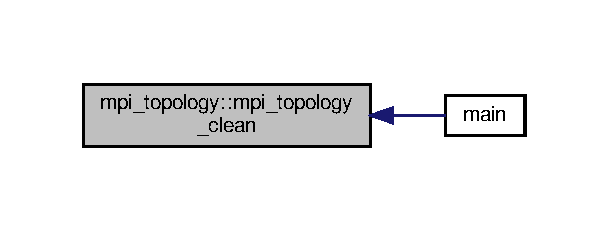
\includegraphics[width=292pt]{namespacempi__topology_aa14e91baaec6d1c1082ebd5ac6e19128_icgraph}
\end{center}
\end{figure}
\mbox{\Hypertarget{namespacempi__topology_a8819f16f50aded913f17520a29d3ec4c}\label{namespacempi__topology_a8819f16f50aded913f17520a29d3ec4c}} 
\index{mpi\+\_\+topology@{mpi\+\_\+topology}!mpi\+\_\+topology\+\_\+make@{mpi\+\_\+topology\+\_\+make}}
\index{mpi\+\_\+topology\+\_\+make@{mpi\+\_\+topology\+\_\+make}!mpi\+\_\+topology@{mpi\+\_\+topology}}
\subsubsection{\texorpdfstring{mpi\+\_\+topology\+\_\+make()}{mpi\_topology\_make()}}
{\footnotesize\ttfamily subroutine, public mpi\+\_\+topology\+::mpi\+\_\+topology\+\_\+make (\begin{DoxyParamCaption}{ }\end{DoxyParamCaption})}



Create the cartesian topology for the M\+PI processes and subcommunicators. 

Here is the caller graph for this function\+:
\nopagebreak
\begin{figure}[H]
\begin{center}
\leavevmode
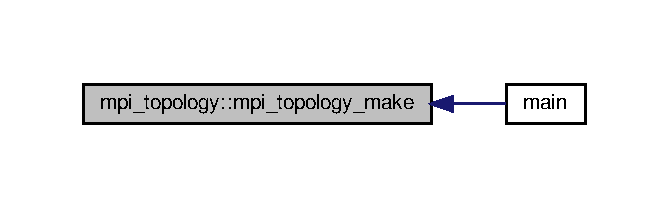
\includegraphics[width=321pt]{namespacempi__topology_a8819f16f50aded913f17520a29d3ec4c_icgraph}
\end{center}
\end{figure}


\subsection{Variable Documentation}
\mbox{\Hypertarget{namespacempi__topology_a4ef8d80f442649d77707d5ebeeefa391}\label{namespacempi__topology_a4ef8d80f442649d77707d5ebeeefa391}} 
\index{mpi\+\_\+topology@{mpi\+\_\+topology}!comm\+\_\+1d\+\_\+x@{comm\+\_\+1d\+\_\+x}}
\index{comm\+\_\+1d\+\_\+x@{comm\+\_\+1d\+\_\+x}!mpi\+\_\+topology@{mpi\+\_\+topology}}
\subsubsection{\texorpdfstring{comm\+\_\+1d\+\_\+x}{comm\_1d\_x}}
{\footnotesize\ttfamily type(\hyperlink{structmpi__topology_1_1cart__comm__1d}{cart\+\_\+comm\+\_\+1d}), public mpi\+\_\+topology\+::comm\+\_\+1d\+\_\+x}



Subcommunicator information in x-\/direction. 

\mbox{\Hypertarget{namespacempi__topology_ad48a88602b9b9950200733823f95b5d0}\label{namespacempi__topology_ad48a88602b9b9950200733823f95b5d0}} 
\index{mpi\+\_\+topology@{mpi\+\_\+topology}!comm\+\_\+1d\+\_\+y@{comm\+\_\+1d\+\_\+y}}
\index{comm\+\_\+1d\+\_\+y@{comm\+\_\+1d\+\_\+y}!mpi\+\_\+topology@{mpi\+\_\+topology}}
\subsubsection{\texorpdfstring{comm\+\_\+1d\+\_\+y}{comm\_1d\_y}}
{\footnotesize\ttfamily type(\hyperlink{structmpi__topology_1_1cart__comm__1d}{cart\+\_\+comm\+\_\+1d}), public mpi\+\_\+topology\+::comm\+\_\+1d\+\_\+y}



Subcommunicator information in y-\/direction. 

\mbox{\Hypertarget{namespacempi__topology_aed5c66dd4697b116c53db4613ad802ce}\label{namespacempi__topology_aed5c66dd4697b116c53db4613ad802ce}} 
\index{mpi\+\_\+topology@{mpi\+\_\+topology}!comm\+\_\+1d\+\_\+z@{comm\+\_\+1d\+\_\+z}}
\index{comm\+\_\+1d\+\_\+z@{comm\+\_\+1d\+\_\+z}!mpi\+\_\+topology@{mpi\+\_\+topology}}
\subsubsection{\texorpdfstring{comm\+\_\+1d\+\_\+z}{comm\_1d\_z}}
{\footnotesize\ttfamily type(\hyperlink{structmpi__topology_1_1cart__comm__1d}{cart\+\_\+comm\+\_\+1d}), public mpi\+\_\+topology\+::comm\+\_\+1d\+\_\+z}



Subcommunicator information in z-\/direction. 

\mbox{\Hypertarget{namespacempi__topology_a2b10bc780ba4b14ea773c36f3e489a94}\label{namespacempi__topology_a2b10bc780ba4b14ea773c36f3e489a94}} 
\index{mpi\+\_\+topology@{mpi\+\_\+topology}!mpi\+\_\+world\+\_\+cart@{mpi\+\_\+world\+\_\+cart}}
\index{mpi\+\_\+world\+\_\+cart@{mpi\+\_\+world\+\_\+cart}!mpi\+\_\+topology@{mpi\+\_\+topology}}
\subsubsection{\texorpdfstring{mpi\+\_\+world\+\_\+cart}{mpi\_world\_cart}}
{\footnotesize\ttfamily integer, public mpi\+\_\+topology\+::mpi\+\_\+world\+\_\+cart}



Communicator for cartesian topology. 

\mbox{\Hypertarget{namespacempi__topology_ac837e97cb4896a72d94eb7a9f12d6682}\label{namespacempi__topology_ac837e97cb4896a72d94eb7a9f12d6682}} 
\index{mpi\+\_\+topology@{mpi\+\_\+topology}!np\+\_\+dim@{np\+\_\+dim}}
\index{np\+\_\+dim@{np\+\_\+dim}!mpi\+\_\+topology@{mpi\+\_\+topology}}
\subsubsection{\texorpdfstring{np\+\_\+dim}{np\_dim}}
{\footnotesize\ttfamily integer, dimension(0\+:2), public mpi\+\_\+topology\+::np\+\_\+dim}



Number of M\+PI processes in 3D topology. 

\mbox{\Hypertarget{namespacempi__topology_ac24cb383bdfbdf566165cf78b03677aa}\label{namespacempi__topology_ac24cb383bdfbdf566165cf78b03677aa}} 
\index{mpi\+\_\+topology@{mpi\+\_\+topology}!period@{period}}
\index{period@{period}!mpi\+\_\+topology@{mpi\+\_\+topology}}
\subsubsection{\texorpdfstring{period}{period}}
{\footnotesize\ttfamily logical, dimension(0\+:2), public mpi\+\_\+topology\+::period}



Periodicity in each direction. 


\hypertarget{namespacenvtx}{}\section{nvtx Module Reference}
\label{namespacenvtx}\index{nvtx@{nvtx}}
\subsection*{Data Types}
\begin{DoxyCompactItemize}
\item 
type \hyperlink{structnvtx_1_1nvtxeventattributes}{nvtxeventattributes}
\item 
interface \hyperlink{interfacenvtx_1_1nvtxrangepop}{nvtxrangepop}
\item 
interface \hyperlink{interfacenvtx_1_1nvtxrangepush}{nvtxrangepush}
\end{DoxyCompactItemize}
\subsection*{Functions/\+Subroutines}
\begin{DoxyCompactItemize}
\item 
subroutine \hyperlink{namespacenvtx_abaf43be3229e42bd0f4c1e75d9670075}{nvtxstartrange} (name, id)
\item 
subroutine \hyperlink{namespacenvtx_aed9b06c5398e0a5b8d7a6e687564fb46}{nvtxendrange}
\end{DoxyCompactItemize}


\subsection{Function/\+Subroutine Documentation}
\mbox{\Hypertarget{namespacenvtx_aed9b06c5398e0a5b8d7a6e687564fb46}\label{namespacenvtx_aed9b06c5398e0a5b8d7a6e687564fb46}} 
\index{nvtx@{nvtx}!nvtxendrange@{nvtxendrange}}
\index{nvtxendrange@{nvtxendrange}!nvtx@{nvtx}}
\subsubsection{\texorpdfstring{nvtxendrange()}{nvtxendrange()}}
{\footnotesize\ttfamily subroutine nvtx\+::nvtxendrange (\begin{DoxyParamCaption}{ }\end{DoxyParamCaption})}

\mbox{\Hypertarget{namespacenvtx_abaf43be3229e42bd0f4c1e75d9670075}\label{namespacenvtx_abaf43be3229e42bd0f4c1e75d9670075}} 
\index{nvtx@{nvtx}!nvtxstartrange@{nvtxstartrange}}
\index{nvtxstartrange@{nvtxstartrange}!nvtx@{nvtx}}
\subsubsection{\texorpdfstring{nvtxstartrange()}{nvtxstartrange()}}
{\footnotesize\ttfamily subroutine nvtx\+::nvtxstartrange (\begin{DoxyParamCaption}\item[{character(kind=c\+\_\+char,len=$\ast$)}]{name,  }\item[{integer, optional}]{id }\end{DoxyParamCaption})}


\hypertarget{namespacepascal__tdma}{}\section{pascal\+\_\+tdma Module Reference}
\label{namespacepascal__tdma}\index{pascal\+\_\+tdma@{pascal\+\_\+tdma}}


Module for Pa\+Sca\+L-\/\+T\+D\+MA library.  


\subsection*{Data Types}
\begin{DoxyCompactItemize}
\item 
type \hyperlink{structpascal__tdma_1_1ptdma__plan__many}{ptdma\+\_\+plan\+\_\+many}
\begin{DoxyCompactList}\small\item\em Execution plan for many tridiagonal systems of equations. \end{DoxyCompactList}\item 
type \hyperlink{structpascal__tdma_1_1ptdma__plan__single}{ptdma\+\_\+plan\+\_\+single}
\begin{DoxyCompactList}\small\item\em Execution plan for a single tridiagonal system of equations. \end{DoxyCompactList}\end{DoxyCompactItemize}
\subsection*{Functions/\+Subroutines}
\begin{DoxyCompactItemize}
\item 
subroutine, public \hyperlink{namespacepascal__tdma_a5dfc2d7c919b47ad364a74d141532a9f}{pascal\+\_\+tdma\+\_\+plan\+\_\+single\+\_\+create} (plan, myrank, nprocs, mpi\+\_\+world, gather\+\_\+rank)
\begin{DoxyCompactList}\small\item\em Create a plan for a single tridiagonal system of equations. \end{DoxyCompactList}\item 
subroutine, public \hyperlink{namespacepascal__tdma_adb04e59c740ce6c4b9518dd86eaeb594}{pascal\+\_\+tdma\+\_\+plan\+\_\+single\+\_\+destroy} (plan)
\begin{DoxyCompactList}\small\item\em Deallocate the allocated arrays in the defined plan\+\_\+single . \end{DoxyCompactList}\item 
subroutine, public \hyperlink{namespacepascal__tdma_a7e9c24b343ae949044eccc8692dcc6e9}{pascal\+\_\+tdma\+\_\+plan\+\_\+many\+\_\+create} (plan, n\+\_\+sys, myrank, nprocs, mpi\+\_\+world)
\begin{DoxyCompactList}\small\item\em Create a plan for many tridiagonal systems of equations. \end{DoxyCompactList}\item 
subroutine, public \hyperlink{namespacepascal__tdma_aceec478e18d25d413a5bd8a174c3fcb8}{pascal\+\_\+tdma\+\_\+plan\+\_\+many\+\_\+destroy} (plan, nprocs)
\begin{DoxyCompactList}\small\item\em Destroy the allocated arrays in the defined plan\+\_\+many. \end{DoxyCompactList}\item 
subroutine, public \hyperlink{namespacepascal__tdma_ab14e132231d4b53fd65dd333ccc85a50}{pascal\+\_\+tdma\+\_\+single\+\_\+solve} (plan, A, B, C, D, n\+\_\+row)
\begin{DoxyCompactList}\small\item\em Solve a single tridiagonal system of equation. \end{DoxyCompactList}\item 
subroutine, public \hyperlink{namespacepascal__tdma_ac8e377fa86c75126380f0196f6046043}{pascal\+\_\+tdma\+\_\+single\+\_\+solve\+\_\+cycle} (plan, A, B, C, D, n\+\_\+row)
\begin{DoxyCompactList}\small\item\em Solve a single cyclic tridiagonal system of equations. \end{DoxyCompactList}\item 
subroutine, public \hyperlink{namespacepascal__tdma_afa0c78b8377f5fe1059907befda3c940}{pascal\+\_\+tdma\+\_\+many\+\_\+solve} (plan, A, B, C, D, n\+\_\+sys, n\+\_\+row)
\begin{DoxyCompactList}\small\item\em Solve many tridiagonal systems of equations. \end{DoxyCompactList}\item 
subroutine, public \hyperlink{namespacepascal__tdma_acbaed65e67ecbfd92a8f1d51d1b69fd5}{pascal\+\_\+tdma\+\_\+many\+\_\+solve\+\_\+cycle} (plan, A, B, C, D, n\+\_\+sys, n\+\_\+row)
\begin{DoxyCompactList}\small\item\em Solve many cyclic tridiagonal systems of equations. \end{DoxyCompactList}\end{DoxyCompactItemize}


\subsection{Detailed Description}
Module for Pa\+Sca\+L-\/\+T\+D\+MA library. 

It contains plans for tridiagonal systems of equations and subroutines for solving them using the defined plans. The operation of the library includes the following three phases\+: (1) Create a data structure called a plan, which has the information for communication and reduced systems. (2) Solve the tridiagonal systems of equations executing from Step 1 to Step 5 (3) Destroy the created plan 

\subsection{Function/\+Subroutine Documentation}
\mbox{\Hypertarget{namespacepascal__tdma_afa0c78b8377f5fe1059907befda3c940}\label{namespacepascal__tdma_afa0c78b8377f5fe1059907befda3c940}} 
\index{pascal\+\_\+tdma@{pascal\+\_\+tdma}!pascal\+\_\+tdma\+\_\+many\+\_\+solve@{pascal\+\_\+tdma\+\_\+many\+\_\+solve}}
\index{pascal\+\_\+tdma\+\_\+many\+\_\+solve@{pascal\+\_\+tdma\+\_\+many\+\_\+solve}!pascal\+\_\+tdma@{pascal\+\_\+tdma}}
\subsubsection{\texorpdfstring{pascal\+\_\+tdma\+\_\+many\+\_\+solve()}{pascal\_tdma\_many\_solve()}}
{\footnotesize\ttfamily subroutine, public pascal\+\_\+tdma\+::pascal\+\_\+tdma\+\_\+many\+\_\+solve (\begin{DoxyParamCaption}\item[{type(\hyperlink{structpascal__tdma_1_1ptdma__plan__many}{ptdma\+\_\+plan\+\_\+many}), intent(inout)}]{plan,  }\item[{double precision, dimension(1\+:n\+\_\+sys,1\+:n\+\_\+row), intent(inout)}]{A,  }\item[{double precision, dimension(1\+:n\+\_\+sys,1\+:n\+\_\+row), intent(inout)}]{B,  }\item[{double precision, dimension(1\+:n\+\_\+sys,1\+:n\+\_\+row), intent(inout)}]{C,  }\item[{double precision, dimension(1\+:n\+\_\+sys,1\+:n\+\_\+row), intent(inout)}]{D,  }\item[{integer, intent(in)}]{n\+\_\+sys,  }\item[{integer, intent(in)}]{n\+\_\+row }\end{DoxyParamCaption})}



Solve many tridiagonal systems of equations. 


\begin{DoxyParams}{Parameters}
{\em plan} & Plan for many tridiagonal systems of equations \\
\hline
{\em A} & Coefficients in lower diagonal elements \\
\hline
{\em B} & Coefficients in diagonal elements \\
\hline
{\em C} & Coefficients in upper diagonal elements \\
\hline
{\em D} & Coefficients in right-\/hand side terms \\
\hline
{\em n\+\_\+sys} & Number of tridiagonal systems per process \\
\hline
{\em n\+\_\+row} & Number of rows in each process, size of a tridiagonal matrix N divided by nprocs \\
\hline
\end{DoxyParams}
Here is the call graph for this function\+:
\nopagebreak
\begin{figure}[H]
\begin{center}
\leavevmode
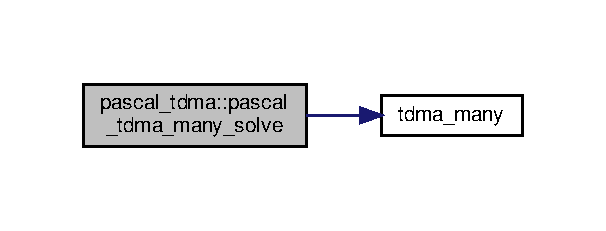
\includegraphics[width=291pt]{namespacepascal__tdma_afa0c78b8377f5fe1059907befda3c940_cgraph}
\end{center}
\end{figure}
Here is the caller graph for this function\+:
\nopagebreak
\begin{figure}[H]
\begin{center}
\leavevmode
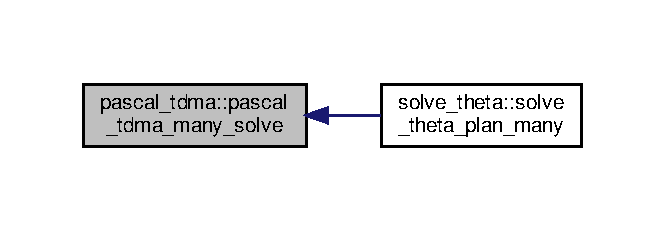
\includegraphics[width=319pt]{namespacepascal__tdma_afa0c78b8377f5fe1059907befda3c940_icgraph}
\end{center}
\end{figure}
\mbox{\Hypertarget{namespacepascal__tdma_acbaed65e67ecbfd92a8f1d51d1b69fd5}\label{namespacepascal__tdma_acbaed65e67ecbfd92a8f1d51d1b69fd5}} 
\index{pascal\+\_\+tdma@{pascal\+\_\+tdma}!pascal\+\_\+tdma\+\_\+many\+\_\+solve\+\_\+cycle@{pascal\+\_\+tdma\+\_\+many\+\_\+solve\+\_\+cycle}}
\index{pascal\+\_\+tdma\+\_\+many\+\_\+solve\+\_\+cycle@{pascal\+\_\+tdma\+\_\+many\+\_\+solve\+\_\+cycle}!pascal\+\_\+tdma@{pascal\+\_\+tdma}}
\subsubsection{\texorpdfstring{pascal\+\_\+tdma\+\_\+many\+\_\+solve\+\_\+cycle()}{pascal\_tdma\_many\_solve\_cycle()}}
{\footnotesize\ttfamily subroutine, public pascal\+\_\+tdma\+::pascal\+\_\+tdma\+\_\+many\+\_\+solve\+\_\+cycle (\begin{DoxyParamCaption}\item[{type(\hyperlink{structpascal__tdma_1_1ptdma__plan__many}{ptdma\+\_\+plan\+\_\+many}), intent(inout)}]{plan,  }\item[{double precision, dimension(1\+:n\+\_\+sys,1\+:n\+\_\+row), intent(inout)}]{A,  }\item[{double precision, dimension(1\+:n\+\_\+sys,1\+:n\+\_\+row), intent(inout)}]{B,  }\item[{double precision, dimension(1\+:n\+\_\+sys,1\+:n\+\_\+row), intent(inout)}]{C,  }\item[{double precision, dimension(1\+:n\+\_\+sys,1\+:n\+\_\+row), intent(inout)}]{D,  }\item[{integer, intent(in)}]{n\+\_\+sys,  }\item[{integer, intent(in)}]{n\+\_\+row }\end{DoxyParamCaption})}



Solve many cyclic tridiagonal systems of equations. 


\begin{DoxyParams}{Parameters}
{\em plan} & Plan for many tridiagonal systems of equations \\
\hline
{\em A} & Coefficients in lower diagonal elements \\
\hline
{\em B} & Coefficients in diagonal elements \\
\hline
{\em C} & Coefficients in upper diagonal elements \\
\hline
{\em D} & Coefficients in right-\/hand side terms \\
\hline
{\em n\+\_\+sys} & Number of tridiagonal systems per process \\
\hline
{\em n\+\_\+row} & Number of rows in each process, size of a tridiagonal matrix N divided by nprocs \\
\hline
\end{DoxyParams}
Here is the call graph for this function\+:
\nopagebreak
\begin{figure}[H]
\begin{center}
\leavevmode
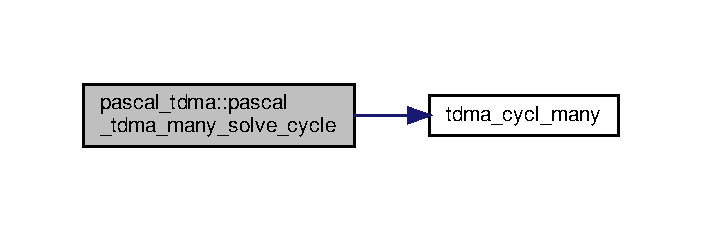
\includegraphics[width=337pt]{namespacepascal__tdma_acbaed65e67ecbfd92a8f1d51d1b69fd5_cgraph}
\end{center}
\end{figure}
Here is the caller graph for this function\+:
\nopagebreak
\begin{figure}[H]
\begin{center}
\leavevmode
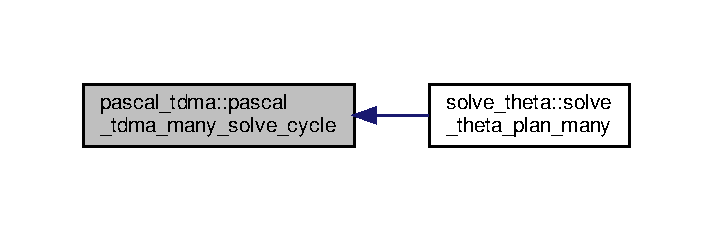
\includegraphics[width=342pt]{namespacepascal__tdma_acbaed65e67ecbfd92a8f1d51d1b69fd5_icgraph}
\end{center}
\end{figure}
\mbox{\Hypertarget{namespacepascal__tdma_a7e9c24b343ae949044eccc8692dcc6e9}\label{namespacepascal__tdma_a7e9c24b343ae949044eccc8692dcc6e9}} 
\index{pascal\+\_\+tdma@{pascal\+\_\+tdma}!pascal\+\_\+tdma\+\_\+plan\+\_\+many\+\_\+create@{pascal\+\_\+tdma\+\_\+plan\+\_\+many\+\_\+create}}
\index{pascal\+\_\+tdma\+\_\+plan\+\_\+many\+\_\+create@{pascal\+\_\+tdma\+\_\+plan\+\_\+many\+\_\+create}!pascal\+\_\+tdma@{pascal\+\_\+tdma}}
\subsubsection{\texorpdfstring{pascal\+\_\+tdma\+\_\+plan\+\_\+many\+\_\+create()}{pascal\_tdma\_plan\_many\_create()}}
{\footnotesize\ttfamily subroutine, public pascal\+\_\+tdma\+::pascal\+\_\+tdma\+\_\+plan\+\_\+many\+\_\+create (\begin{DoxyParamCaption}\item[{type(\hyperlink{structpascal__tdma_1_1ptdma__plan__many}{ptdma\+\_\+plan\+\_\+many}), intent(inout)}]{plan,  }\item[{integer, intent(in)}]{n\+\_\+sys,  }\item[{integer, intent(in)}]{myrank,  }\item[{integer, intent(in)}]{nprocs,  }\item[{integer, intent(in)}]{mpi\+\_\+world }\end{DoxyParamCaption})}



Create a plan for many tridiagonal systems of equations. 


\begin{DoxyParams}{Parameters}
{\em plan} & Plan for a single tridiagonal system of equations \\
\hline
{\em n\+\_\+sys} & Number of tridiagonal systems of equations for process \\
\hline
{\em myrank} & Rank ID in mpi\+\_\+world \\
\hline
{\em nprocs} & Number of M\+PI process in mpi\+\_\+world \\
\hline
{\em mpi\+\_\+world} & Communicator for M\+P\+I\+\_\+\+Gather and M\+P\+I\+\_\+\+Scatter of reduced equations \\
\hline
\end{DoxyParams}
Here is the call graph for this function\+:
\nopagebreak
\begin{figure}[H]
\begin{center}
\leavevmode
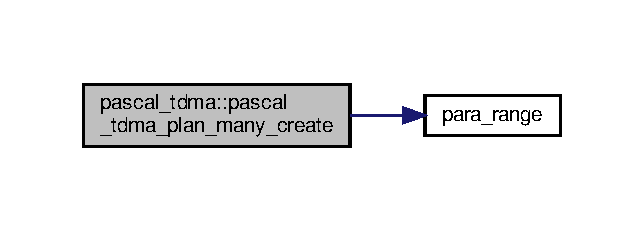
\includegraphics[width=309pt]{namespacepascal__tdma_a7e9c24b343ae949044eccc8692dcc6e9_cgraph}
\end{center}
\end{figure}
Here is the caller graph for this function\+:
\nopagebreak
\begin{figure}[H]
\begin{center}
\leavevmode
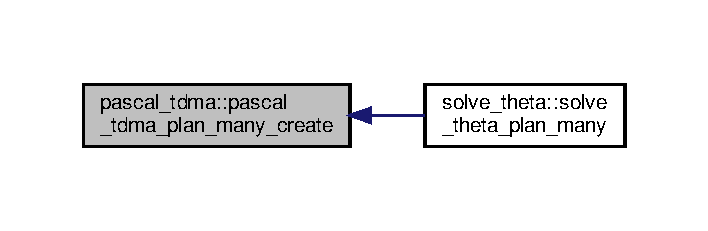
\includegraphics[width=340pt]{namespacepascal__tdma_a7e9c24b343ae949044eccc8692dcc6e9_icgraph}
\end{center}
\end{figure}
\mbox{\Hypertarget{namespacepascal__tdma_aceec478e18d25d413a5bd8a174c3fcb8}\label{namespacepascal__tdma_aceec478e18d25d413a5bd8a174c3fcb8}} 
\index{pascal\+\_\+tdma@{pascal\+\_\+tdma}!pascal\+\_\+tdma\+\_\+plan\+\_\+many\+\_\+destroy@{pascal\+\_\+tdma\+\_\+plan\+\_\+many\+\_\+destroy}}
\index{pascal\+\_\+tdma\+\_\+plan\+\_\+many\+\_\+destroy@{pascal\+\_\+tdma\+\_\+plan\+\_\+many\+\_\+destroy}!pascal\+\_\+tdma@{pascal\+\_\+tdma}}
\subsubsection{\texorpdfstring{pascal\+\_\+tdma\+\_\+plan\+\_\+many\+\_\+destroy()}{pascal\_tdma\_plan\_many\_destroy()}}
{\footnotesize\ttfamily subroutine, public pascal\+\_\+tdma\+::pascal\+\_\+tdma\+\_\+plan\+\_\+many\+\_\+destroy (\begin{DoxyParamCaption}\item[{type(\hyperlink{structpascal__tdma_1_1ptdma__plan__many}{ptdma\+\_\+plan\+\_\+many}), intent(inout)}]{plan,  }\item[{integer}]{nprocs }\end{DoxyParamCaption})}



Destroy the allocated arrays in the defined plan\+\_\+many. 


\begin{DoxyParams}{Parameters}
{\em plan} & Plan for many tridiagonal systems of equations \\
\hline
\end{DoxyParams}
Here is the caller graph for this function\+:
\nopagebreak
\begin{figure}[H]
\begin{center}
\leavevmode
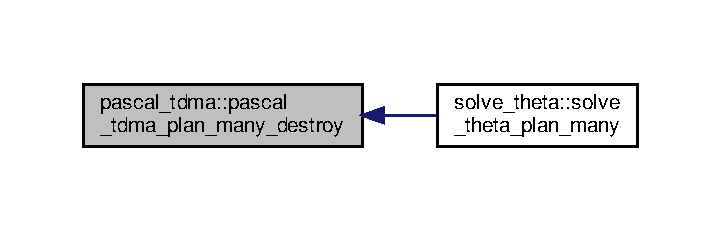
\includegraphics[width=346pt]{namespacepascal__tdma_aceec478e18d25d413a5bd8a174c3fcb8_icgraph}
\end{center}
\end{figure}
\mbox{\Hypertarget{namespacepascal__tdma_a5dfc2d7c919b47ad364a74d141532a9f}\label{namespacepascal__tdma_a5dfc2d7c919b47ad364a74d141532a9f}} 
\index{pascal\+\_\+tdma@{pascal\+\_\+tdma}!pascal\+\_\+tdma\+\_\+plan\+\_\+single\+\_\+create@{pascal\+\_\+tdma\+\_\+plan\+\_\+single\+\_\+create}}
\index{pascal\+\_\+tdma\+\_\+plan\+\_\+single\+\_\+create@{pascal\+\_\+tdma\+\_\+plan\+\_\+single\+\_\+create}!pascal\+\_\+tdma@{pascal\+\_\+tdma}}
\subsubsection{\texorpdfstring{pascal\+\_\+tdma\+\_\+plan\+\_\+single\+\_\+create()}{pascal\_tdma\_plan\_single\_create()}}
{\footnotesize\ttfamily subroutine, public pascal\+\_\+tdma\+::pascal\+\_\+tdma\+\_\+plan\+\_\+single\+\_\+create (\begin{DoxyParamCaption}\item[{type(\hyperlink{structpascal__tdma_1_1ptdma__plan__single}{ptdma\+\_\+plan\+\_\+single}), intent(inout)}]{plan,  }\item[{integer, intent(in)}]{myrank,  }\item[{integer, intent(in)}]{nprocs,  }\item[{integer, intent(in)}]{mpi\+\_\+world,  }\item[{integer, intent(in)}]{gather\+\_\+rank }\end{DoxyParamCaption})}



Create a plan for a single tridiagonal system of equations. 


\begin{DoxyParams}{Parameters}
{\em plan} & Plan for a single tridiagonal system of equations \\
\hline
{\em myrank} & Rank ID in mpi\+\_\+world \\
\hline
{\em nprocs} & Number of M\+PI process in mpi\+\_\+world \\
\hline
{\em mpi\+\_\+world} & Communicator for M\+P\+I\+\_\+\+Gather and M\+P\+I\+\_\+\+Scatter of a reduced system \\
\hline
{\em gather\+\_\+rank} & Target rank where all coefficients are gathered to \\
\hline
\end{DoxyParams}
Here is the caller graph for this function\+:
\nopagebreak
\begin{figure}[H]
\begin{center}
\leavevmode
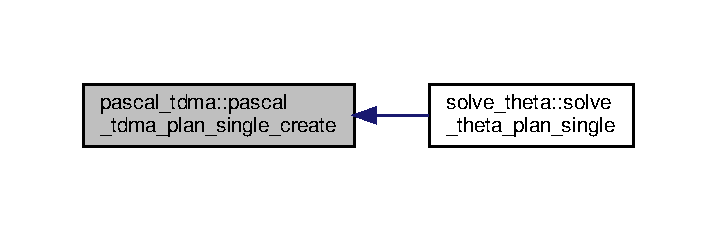
\includegraphics[width=344pt]{namespacepascal__tdma_a5dfc2d7c919b47ad364a74d141532a9f_icgraph}
\end{center}
\end{figure}
\mbox{\Hypertarget{namespacepascal__tdma_adb04e59c740ce6c4b9518dd86eaeb594}\label{namespacepascal__tdma_adb04e59c740ce6c4b9518dd86eaeb594}} 
\index{pascal\+\_\+tdma@{pascal\+\_\+tdma}!pascal\+\_\+tdma\+\_\+plan\+\_\+single\+\_\+destroy@{pascal\+\_\+tdma\+\_\+plan\+\_\+single\+\_\+destroy}}
\index{pascal\+\_\+tdma\+\_\+plan\+\_\+single\+\_\+destroy@{pascal\+\_\+tdma\+\_\+plan\+\_\+single\+\_\+destroy}!pascal\+\_\+tdma@{pascal\+\_\+tdma}}
\subsubsection{\texorpdfstring{pascal\+\_\+tdma\+\_\+plan\+\_\+single\+\_\+destroy()}{pascal\_tdma\_plan\_single\_destroy()}}
{\footnotesize\ttfamily subroutine, public pascal\+\_\+tdma\+::pascal\+\_\+tdma\+\_\+plan\+\_\+single\+\_\+destroy (\begin{DoxyParamCaption}\item[{type(\hyperlink{structpascal__tdma_1_1ptdma__plan__single}{ptdma\+\_\+plan\+\_\+single}), intent(inout)}]{plan }\end{DoxyParamCaption})}



Deallocate the allocated arrays in the defined plan\+\_\+single . 


\begin{DoxyParams}{Parameters}
{\em plan} & Plan for a single tridiagonal system of equations \\
\hline
\end{DoxyParams}
Here is the caller graph for this function\+:
\nopagebreak
\begin{figure}[H]
\begin{center}
\leavevmode
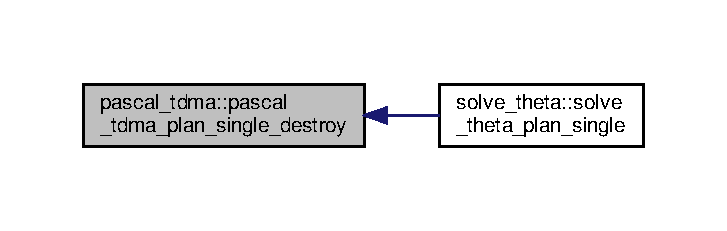
\includegraphics[width=349pt]{namespacepascal__tdma_adb04e59c740ce6c4b9518dd86eaeb594_icgraph}
\end{center}
\end{figure}
\mbox{\Hypertarget{namespacepascal__tdma_ab14e132231d4b53fd65dd333ccc85a50}\label{namespacepascal__tdma_ab14e132231d4b53fd65dd333ccc85a50}} 
\index{pascal\+\_\+tdma@{pascal\+\_\+tdma}!pascal\+\_\+tdma\+\_\+single\+\_\+solve@{pascal\+\_\+tdma\+\_\+single\+\_\+solve}}
\index{pascal\+\_\+tdma\+\_\+single\+\_\+solve@{pascal\+\_\+tdma\+\_\+single\+\_\+solve}!pascal\+\_\+tdma@{pascal\+\_\+tdma}}
\subsubsection{\texorpdfstring{pascal\+\_\+tdma\+\_\+single\+\_\+solve()}{pascal\_tdma\_single\_solve()}}
{\footnotesize\ttfamily subroutine, public pascal\+\_\+tdma\+::pascal\+\_\+tdma\+\_\+single\+\_\+solve (\begin{DoxyParamCaption}\item[{type(\hyperlink{structpascal__tdma_1_1ptdma__plan__single}{ptdma\+\_\+plan\+\_\+single}), intent(inout)}]{plan,  }\item[{double precision, dimension(1\+:n\+\_\+row), intent(inout)}]{A,  }\item[{double precision, dimension(1\+:n\+\_\+row), intent(inout)}]{B,  }\item[{double precision, dimension(1\+:n\+\_\+row), intent(inout)}]{C,  }\item[{double precision, dimension(1\+:n\+\_\+row), intent(inout)}]{D,  }\item[{integer, intent(in)}]{n\+\_\+row }\end{DoxyParamCaption})}



Solve a single tridiagonal system of equation. 


\begin{DoxyParams}{Parameters}
{\em plan} & Plan for a single tridiagonal system of equation \\
\hline
{\em A} & Coefficients in lower diagonal elements \\
\hline
{\em B} & Coefficients in diagonal elements \\
\hline
{\em C} & Coefficients in upper diagonal elements \\
\hline
{\em D} & Coefficients in right-\/hand side terms \\
\hline
{\em n\+\_\+row} & Number of rows in each process, size of a tridiagonal matrix N divided by nprocs \\
\hline
\end{DoxyParams}
Here is the call graph for this function\+:
\nopagebreak
\begin{figure}[H]
\begin{center}
\leavevmode
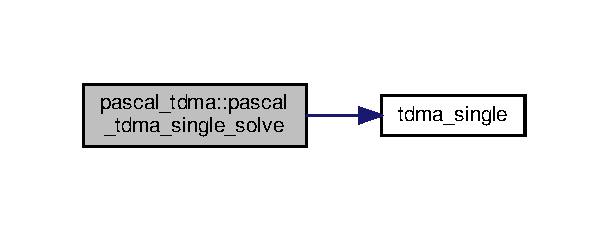
\includegraphics[width=292pt]{namespacepascal__tdma_ab14e132231d4b53fd65dd333ccc85a50_cgraph}
\end{center}
\end{figure}
Here is the caller graph for this function\+:
\nopagebreak
\begin{figure}[H]
\begin{center}
\leavevmode
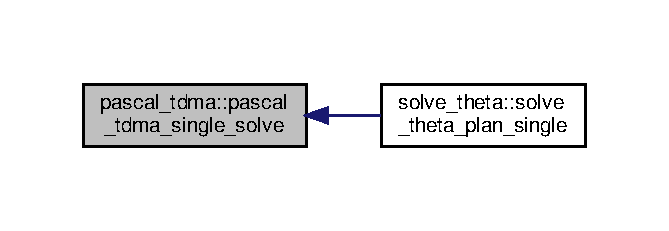
\includegraphics[width=321pt]{namespacepascal__tdma_ab14e132231d4b53fd65dd333ccc85a50_icgraph}
\end{center}
\end{figure}
\mbox{\Hypertarget{namespacepascal__tdma_ac8e377fa86c75126380f0196f6046043}\label{namespacepascal__tdma_ac8e377fa86c75126380f0196f6046043}} 
\index{pascal\+\_\+tdma@{pascal\+\_\+tdma}!pascal\+\_\+tdma\+\_\+single\+\_\+solve\+\_\+cycle@{pascal\+\_\+tdma\+\_\+single\+\_\+solve\+\_\+cycle}}
\index{pascal\+\_\+tdma\+\_\+single\+\_\+solve\+\_\+cycle@{pascal\+\_\+tdma\+\_\+single\+\_\+solve\+\_\+cycle}!pascal\+\_\+tdma@{pascal\+\_\+tdma}}
\subsubsection{\texorpdfstring{pascal\+\_\+tdma\+\_\+single\+\_\+solve\+\_\+cycle()}{pascal\_tdma\_single\_solve\_cycle()}}
{\footnotesize\ttfamily subroutine, public pascal\+\_\+tdma\+::pascal\+\_\+tdma\+\_\+single\+\_\+solve\+\_\+cycle (\begin{DoxyParamCaption}\item[{type(\hyperlink{structpascal__tdma_1_1ptdma__plan__single}{ptdma\+\_\+plan\+\_\+single}), intent(inout)}]{plan,  }\item[{double precision, dimension(1\+:n\+\_\+row), intent(inout)}]{A,  }\item[{double precision, dimension(1\+:n\+\_\+row), intent(inout)}]{B,  }\item[{double precision, dimension(1\+:n\+\_\+row), intent(inout)}]{C,  }\item[{double precision, dimension(1\+:n\+\_\+row), intent(inout)}]{D,  }\item[{integer, intent(in)}]{n\+\_\+row }\end{DoxyParamCaption})}



Solve a single cyclic tridiagonal system of equations. 


\begin{DoxyParams}{Parameters}
{\em plan} & Plan for a single tridiagonal system of equations \\
\hline
{\em A} & Coefficients in lower diagonal elements \\
\hline
{\em B} & Coefficients in diagonal elements \\
\hline
{\em C} & Coefficients in upper diagonal elements \\
\hline
{\em D} & Coefficients in right-\/hand side terms \\
\hline
{\em n\+\_\+row} & Number of rows in each process, size of a tridiagonal matrix N divided by nprocs \\
\hline
\end{DoxyParams}
Here is the call graph for this function\+:
\nopagebreak
\begin{figure}[H]
\begin{center}
\leavevmode
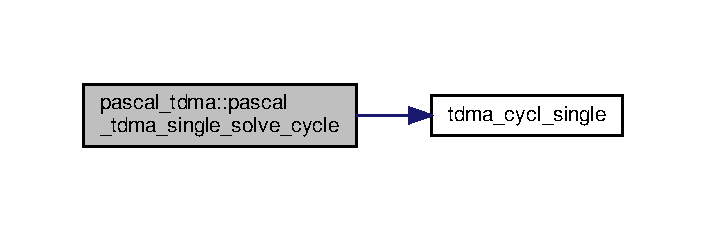
\includegraphics[width=339pt]{namespacepascal__tdma_ac8e377fa86c75126380f0196f6046043_cgraph}
\end{center}
\end{figure}
Here is the caller graph for this function\+:
\nopagebreak
\begin{figure}[H]
\begin{center}
\leavevmode
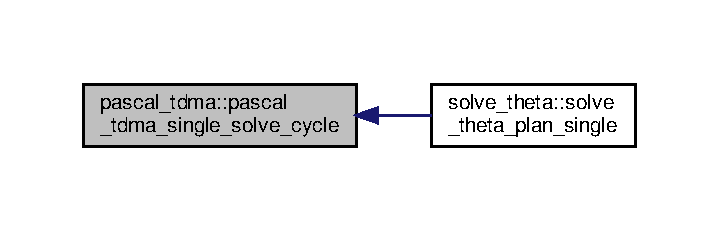
\includegraphics[width=345pt]{namespacepascal__tdma_ac8e377fa86c75126380f0196f6046043_icgraph}
\end{center}
\end{figure}

\hypertarget{namespacepascal__tdma__cuda}{}\section{pascal\+\_\+tdma\+\_\+cuda Module Reference}
\label{namespacepascal__tdma__cuda}\index{pascal\+\_\+tdma\+\_\+cuda@{pascal\+\_\+tdma\+\_\+cuda}}


Module for Pa\+Sca\+L\+\_\+\+T\+D\+MA library with C\+U\+DA.  


\subsection*{Data Types}
\begin{DoxyCompactItemize}
\item 
type \hyperlink{structpascal__tdma__cuda_1_1ptdma__plan__many__cuda}{ptdma\+\_\+plan\+\_\+many\+\_\+cuda}
\begin{DoxyCompactList}\small\item\em Execution plan for many tridiagonal systems of equations. \end{DoxyCompactList}\end{DoxyCompactItemize}
\subsection*{Functions/\+Subroutines}
\textbf{ }\par
\begin{DoxyCompactItemize}
\item 
subroutine, public \hyperlink{namespacepascal__tdma__cuda_a84c442c238f7d1a18eef430aaa15e6c1}{pascal\+\_\+tdma\+\_\+plan\+\_\+many\+\_\+create\+\_\+cuda} (p, nx\+\_\+sys, ny\+\_\+sys, nz\+\_\+row, myrank, nprocs, mpi\+\_\+world, thread\+\_\+in)
\begin{DoxyCompactList}\small\item\em Create a plan for many tridiagonal systems of equations. \end{DoxyCompactList}\item 
subroutine, public \hyperlink{namespacepascal__tdma__cuda_a70734ba15cf5a093ac3ba2ccbc4f5330}{pascal\+\_\+tdma\+\_\+plan\+\_\+many\+\_\+destroy\+\_\+cuda} (p)
\begin{DoxyCompactList}\small\item\em Destroy the allocated arrays in the defined plan\+\_\+many. \end{DoxyCompactList}\item 
subroutine, public \hyperlink{namespacepascal__tdma__cuda_a0043d538e133925d9a37bf7bcdaf4b08}{pascal\+\_\+tdma\+\_\+many\+\_\+solve\+\_\+cuda} (p, a\+\_\+d, b\+\_\+d, c\+\_\+d, d\+\_\+d)
\begin{DoxyCompactList}\small\item\em Solve many tridiagonal systems of equations. \end{DoxyCompactList}\item 
subroutine, public \hyperlink{namespacepascal__tdma__cuda_afdd30998c4a8aecc093c823e3212b57a}{pascal\+\_\+tdma\+\_\+many\+\_\+solve\+\_\+cycle\+\_\+cuda} (p, a\+\_\+d, b\+\_\+d, c\+\_\+d, d\+\_\+d)
\begin{DoxyCompactList}\small\item\em Solve many cyclic tridiagonal systems of equations. \end{DoxyCompactList}\end{DoxyCompactItemize}



\subsection{Detailed Description}
Module for Pa\+Sca\+L\+\_\+\+T\+D\+MA library with C\+U\+DA. 

It contains plans for tridiagonal systems of equations and subroutines for solving them using the defined plans. The operation of the library includes the following three phases\+: (1) Create a data structure called a plan with the information for communication and reduced systems. (2) Solve the tridiagonal systems of equations executing from Step 1 to Step 5 (3) Destroy the created plan 

\subsection{Function/\+Subroutine Documentation}
\mbox{\Hypertarget{namespacepascal__tdma__cuda_a0043d538e133925d9a37bf7bcdaf4b08}\label{namespacepascal__tdma__cuda_a0043d538e133925d9a37bf7bcdaf4b08}} 
\index{pascal\+\_\+tdma\+\_\+cuda@{pascal\+\_\+tdma\+\_\+cuda}!pascal\+\_\+tdma\+\_\+many\+\_\+solve\+\_\+cuda@{pascal\+\_\+tdma\+\_\+many\+\_\+solve\+\_\+cuda}}
\index{pascal\+\_\+tdma\+\_\+many\+\_\+solve\+\_\+cuda@{pascal\+\_\+tdma\+\_\+many\+\_\+solve\+\_\+cuda}!pascal\+\_\+tdma\+\_\+cuda@{pascal\+\_\+tdma\+\_\+cuda}}
\subsubsection{\texorpdfstring{pascal\+\_\+tdma\+\_\+many\+\_\+solve\+\_\+cuda()}{pascal\_tdma\_many\_solve\_cuda()}}
{\footnotesize\ttfamily subroutine, public pascal\+\_\+tdma\+\_\+cuda\+::pascal\+\_\+tdma\+\_\+many\+\_\+solve\+\_\+cuda (\begin{DoxyParamCaption}\item[{type(\hyperlink{structpascal__tdma__cuda_1_1ptdma__plan__many__cuda}{ptdma\+\_\+plan\+\_\+many\+\_\+cuda}), intent(inout)}]{p,  }\item[{double precision, dimension(\+:, \+:, \+:)}]{a\+\_\+d,  }\item[{double precision, dimension(\+:, \+:, \+:)}]{b\+\_\+d,  }\item[{double precision, dimension(\+:, \+:, \+:)}]{c\+\_\+d,  }\item[{double precision, dimension(\+:, \+:, \+:)}]{d\+\_\+d }\end{DoxyParamCaption})}



Solve many tridiagonal systems of equations. 


\begin{DoxyParams}{Parameters}
{\em p} & Plan for many tridiagonal systems of equations \\
\hline
{\em a\+\_\+d} & Coefficient array of lower diagonal elements \\
\hline
{\em b\+\_\+d} & Coefficient array of diagonal elements \\
\hline
{\em c\+\_\+d} & Coefficient array of upper diagonal elements \\
\hline
{\em d\+\_\+d} & Coefficient array of right-\/hand side terms \\
\hline
\end{DoxyParams}
Here is the caller graph for this function\+:
\nopagebreak
\begin{figure}[H]
\begin{center}
\leavevmode
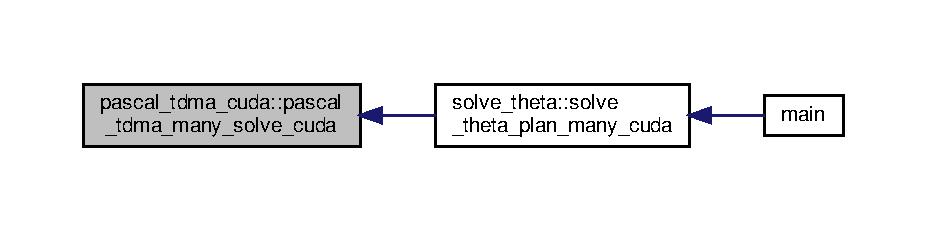
\includegraphics[width=350pt]{namespacepascal__tdma__cuda_a0043d538e133925d9a37bf7bcdaf4b08_icgraph}
\end{center}
\end{figure}
\mbox{\Hypertarget{namespacepascal__tdma__cuda_afdd30998c4a8aecc093c823e3212b57a}\label{namespacepascal__tdma__cuda_afdd30998c4a8aecc093c823e3212b57a}} 
\index{pascal\+\_\+tdma\+\_\+cuda@{pascal\+\_\+tdma\+\_\+cuda}!pascal\+\_\+tdma\+\_\+many\+\_\+solve\+\_\+cycle\+\_\+cuda@{pascal\+\_\+tdma\+\_\+many\+\_\+solve\+\_\+cycle\+\_\+cuda}}
\index{pascal\+\_\+tdma\+\_\+many\+\_\+solve\+\_\+cycle\+\_\+cuda@{pascal\+\_\+tdma\+\_\+many\+\_\+solve\+\_\+cycle\+\_\+cuda}!pascal\+\_\+tdma\+\_\+cuda@{pascal\+\_\+tdma\+\_\+cuda}}
\subsubsection{\texorpdfstring{pascal\+\_\+tdma\+\_\+many\+\_\+solve\+\_\+cycle\+\_\+cuda()}{pascal\_tdma\_many\_solve\_cycle\_cuda()}}
{\footnotesize\ttfamily subroutine, public pascal\+\_\+tdma\+\_\+cuda\+::pascal\+\_\+tdma\+\_\+many\+\_\+solve\+\_\+cycle\+\_\+cuda (\begin{DoxyParamCaption}\item[{type(\hyperlink{structpascal__tdma__cuda_1_1ptdma__plan__many__cuda}{ptdma\+\_\+plan\+\_\+many\+\_\+cuda}), intent(inout)}]{p,  }\item[{double precision, dimension(\+:, \+:, \+:)}]{a\+\_\+d,  }\item[{double precision, dimension(\+:, \+:, \+:)}]{b\+\_\+d,  }\item[{double precision, dimension(\+:, \+:, \+:)}]{c\+\_\+d,  }\item[{double precision, dimension(\+:, \+:, \+:)}]{d\+\_\+d }\end{DoxyParamCaption})}



Solve many cyclic tridiagonal systems of equations. 


\begin{DoxyParams}{Parameters}
{\em p} & Plan for many tridiagonal systems of equations \\
\hline
{\em a\+\_\+d} & Coefficient array of lower diagonal elements \\
\hline
{\em b\+\_\+d} & Coefficient array of diagonal elements \\
\hline
{\em c\+\_\+d} & Coefficient array of upper diagonal elements \\
\hline
{\em d\+\_\+d} & Coefficient array of right-\/hand side terms \\
\hline
\end{DoxyParams}
Here is the caller graph for this function\+:
\nopagebreak
\begin{figure}[H]
\begin{center}
\leavevmode
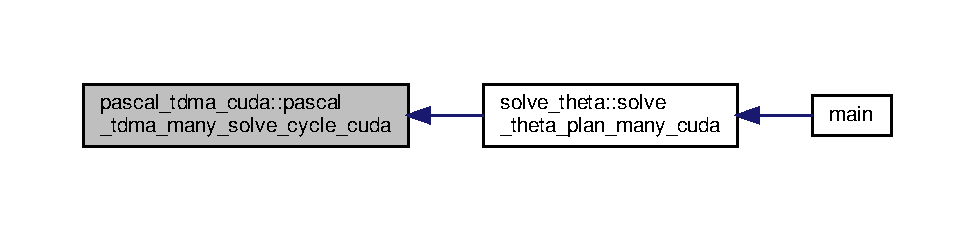
\includegraphics[width=350pt]{namespacepascal__tdma__cuda_afdd30998c4a8aecc093c823e3212b57a_icgraph}
\end{center}
\end{figure}
\mbox{\Hypertarget{namespacepascal__tdma__cuda_a84c442c238f7d1a18eef430aaa15e6c1}\label{namespacepascal__tdma__cuda_a84c442c238f7d1a18eef430aaa15e6c1}} 
\index{pascal\+\_\+tdma\+\_\+cuda@{pascal\+\_\+tdma\+\_\+cuda}!pascal\+\_\+tdma\+\_\+plan\+\_\+many\+\_\+create\+\_\+cuda@{pascal\+\_\+tdma\+\_\+plan\+\_\+many\+\_\+create\+\_\+cuda}}
\index{pascal\+\_\+tdma\+\_\+plan\+\_\+many\+\_\+create\+\_\+cuda@{pascal\+\_\+tdma\+\_\+plan\+\_\+many\+\_\+create\+\_\+cuda}!pascal\+\_\+tdma\+\_\+cuda@{pascal\+\_\+tdma\+\_\+cuda}}
\subsubsection{\texorpdfstring{pascal\+\_\+tdma\+\_\+plan\+\_\+many\+\_\+create\+\_\+cuda()}{pascal\_tdma\_plan\_many\_create\_cuda()}}
{\footnotesize\ttfamily subroutine, public pascal\+\_\+tdma\+\_\+cuda\+::pascal\+\_\+tdma\+\_\+plan\+\_\+many\+\_\+create\+\_\+cuda (\begin{DoxyParamCaption}\item[{type(\hyperlink{structpascal__tdma__cuda_1_1ptdma__plan__many__cuda}{ptdma\+\_\+plan\+\_\+many\+\_\+cuda}), intent(inout)}]{p,  }\item[{integer, intent(in)}]{nx\+\_\+sys,  }\item[{integer, intent(in)}]{ny\+\_\+sys,  }\item[{integer, intent(in)}]{nz\+\_\+row,  }\item[{integer, intent(in)}]{myrank,  }\item[{integer, intent(in)}]{nprocs,  }\item[{integer, intent(in)}]{mpi\+\_\+world,  }\item[{type(dim3)}]{thread\+\_\+in }\end{DoxyParamCaption})}



Create a plan for many tridiagonal systems of equations. 


\begin{DoxyParams}{Parameters}
{\em p} & Plan for a many tridiagonal system of equations \\
\hline
{\em nx\+\_\+sys} & Number of tridiagonal systems of equations in x-\/direction per process \\
\hline
{\em ny\+\_\+sys} & Number of tridiagonal systems of equations in y-\/direction per process \\
\hline
{\em nz\+\_\+row} & Row size of partitioned tridiagonal matrix in z-\/direction per process \\
\hline
{\em myrank} & Rank ID in mpi\+\_\+world \\
\hline
{\em nprocs} & Number of M\+PI process in mpi\+\_\+world \\
\hline
{\em mpi\+\_\+world} & Communicator for M\+P\+I\+\_\+\+Gather and M\+P\+I\+\_\+\+Scatter of reduced equations \\
\hline
\end{DoxyParams}
Here is the call graph for this function\+:
\nopagebreak
\begin{figure}[H]
\begin{center}
\leavevmode
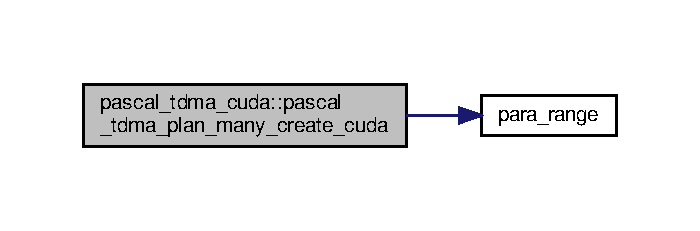
\includegraphics[width=336pt]{namespacepascal__tdma__cuda_a84c442c238f7d1a18eef430aaa15e6c1_cgraph}
\end{center}
\end{figure}
Here is the caller graph for this function\+:
\nopagebreak
\begin{figure}[H]
\begin{center}
\leavevmode
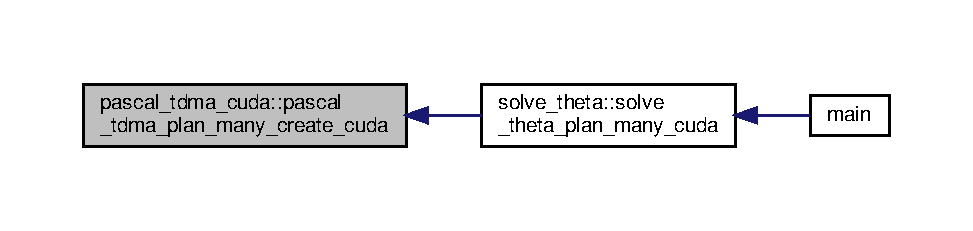
\includegraphics[width=350pt]{namespacepascal__tdma__cuda_a84c442c238f7d1a18eef430aaa15e6c1_icgraph}
\end{center}
\end{figure}
\mbox{\Hypertarget{namespacepascal__tdma__cuda_a70734ba15cf5a093ac3ba2ccbc4f5330}\label{namespacepascal__tdma__cuda_a70734ba15cf5a093ac3ba2ccbc4f5330}} 
\index{pascal\+\_\+tdma\+\_\+cuda@{pascal\+\_\+tdma\+\_\+cuda}!pascal\+\_\+tdma\+\_\+plan\+\_\+many\+\_\+destroy\+\_\+cuda@{pascal\+\_\+tdma\+\_\+plan\+\_\+many\+\_\+destroy\+\_\+cuda}}
\index{pascal\+\_\+tdma\+\_\+plan\+\_\+many\+\_\+destroy\+\_\+cuda@{pascal\+\_\+tdma\+\_\+plan\+\_\+many\+\_\+destroy\+\_\+cuda}!pascal\+\_\+tdma\+\_\+cuda@{pascal\+\_\+tdma\+\_\+cuda}}
\subsubsection{\texorpdfstring{pascal\+\_\+tdma\+\_\+plan\+\_\+many\+\_\+destroy\+\_\+cuda()}{pascal\_tdma\_plan\_many\_destroy\_cuda()}}
{\footnotesize\ttfamily subroutine, public pascal\+\_\+tdma\+\_\+cuda\+::pascal\+\_\+tdma\+\_\+plan\+\_\+many\+\_\+destroy\+\_\+cuda (\begin{DoxyParamCaption}\item[{type(\hyperlink{structpascal__tdma__cuda_1_1ptdma__plan__many__cuda}{ptdma\+\_\+plan\+\_\+many\+\_\+cuda}), intent(inout)}]{p }\end{DoxyParamCaption})}



Destroy the allocated arrays in the defined plan\+\_\+many. 


\begin{DoxyParams}{Parameters}
{\em p} & Plan for many tridiagonal systems of equations \\
\hline
\end{DoxyParams}
Here is the caller graph for this function\+:
\nopagebreak
\begin{figure}[H]
\begin{center}
\leavevmode
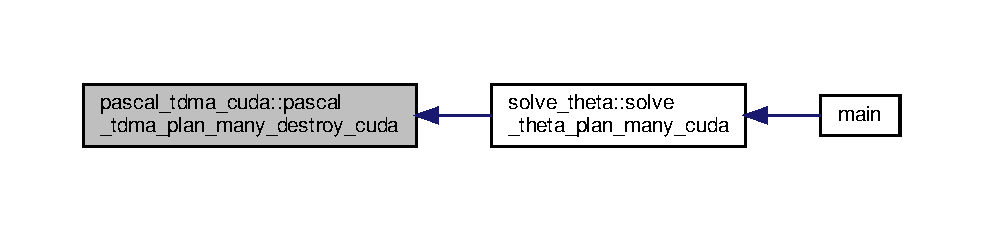
\includegraphics[width=350pt]{namespacepascal__tdma__cuda_a70734ba15cf5a093ac3ba2ccbc4f5330_icgraph}
\end{center}
\end{figure}

\hypertarget{namespacesolve__theta}{}\section{solve\+\_\+theta Module Reference}
\label{namespacesolve__theta}\index{solve\+\_\+theta@{solve\+\_\+theta}}
\subsection*{Functions/\+Subroutines}
\begin{DoxyCompactItemize}
\item 
subroutine, public \hyperlink{namespacesolve__theta_a215d44e312ec3ab2a3ab44fa0613b100}{solve\+\_\+theta\+\_\+plan\+\_\+single} (theta)
\begin{DoxyCompactList}\small\item\em An example solver for a single tridiagonal system of equations using Pa\+Sca\+L\+\_\+\+T\+D\+MA. \end{DoxyCompactList}\item 
subroutine, public \hyperlink{namespacesolve__theta_a0b7fdb576c007dc344092bf40efb0f4b}{solve\+\_\+theta\+\_\+plan\+\_\+many} (theta)
\begin{DoxyCompactList}\small\item\em An example solver for many tridiagonal systems of equations using Pa\+Sca\+L\+\_\+\+T\+D\+MA. \end{DoxyCompactList}\item 
subroutine, public \hyperlink{namespacesolve__theta_a84c4bdc671112259790470f6ad4c7e4c}{solve\+\_\+theta\+\_\+plan\+\_\+many\+\_\+cuda} (theta)
\begin{DoxyCompactList}\small\item\em An example solver for many tridiagonal systems of equations using Pa\+Sca\+L\+\_\+\+T\+D\+MA with C\+U\+DA. \end{DoxyCompactList}\item 
subroutine \hyperlink{namespacesolve__theta_a75284cf6dd015edde5309be8368c4c9e}{ghostcell\+\_\+update\+\_\+cuda} (Value\+\_\+sub\+\_\+d)
\begin{DoxyCompactList}\small\item\em Ghost cell update in device. \end{DoxyCompactList}\end{DoxyCompactItemize}


\subsection{Function/\+Subroutine Documentation}
\mbox{\Hypertarget{namespacesolve__theta_a75284cf6dd015edde5309be8368c4c9e}\label{namespacesolve__theta_a75284cf6dd015edde5309be8368c4c9e}} 
\index{solve\+\_\+theta@{solve\+\_\+theta}!ghostcell\+\_\+update\+\_\+cuda@{ghostcell\+\_\+update\+\_\+cuda}}
\index{ghostcell\+\_\+update\+\_\+cuda@{ghostcell\+\_\+update\+\_\+cuda}!solve\+\_\+theta@{solve\+\_\+theta}}
\subsubsection{\texorpdfstring{ghostcell\+\_\+update\+\_\+cuda()}{ghostcell\_update\_cuda()}}
{\footnotesize\ttfamily subroutine solve\+\_\+theta\+::ghostcell\+\_\+update\+\_\+cuda (\begin{DoxyParamCaption}\item[{double precision}]{Value\+\_\+sub\+\_\+d }\end{DoxyParamCaption})}



Ghost cell update in device. 

This subroutine is to update the ghost-\/cell in the device. Allocated buffers in device memory are used. 
\begin{DoxyParams}{Parameters}
{\em Value\+\_\+sub\+\_\+d} & Main 3-\/D variable to be updated with GC \\
\hline
\end{DoxyParams}
Here is the caller graph for this function\+:
\nopagebreak
\begin{figure}[H]
\begin{center}
\leavevmode
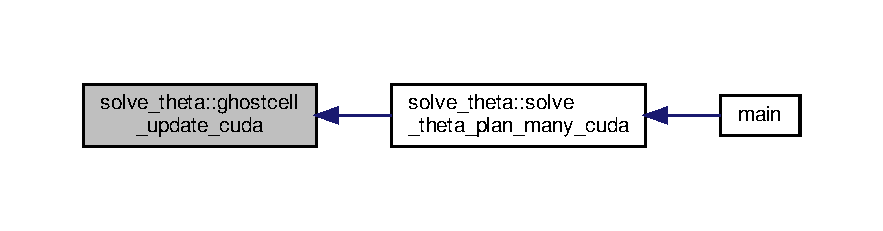
\includegraphics[width=350pt]{namespacesolve__theta_a75284cf6dd015edde5309be8368c4c9e_icgraph}
\end{center}
\end{figure}
\mbox{\Hypertarget{namespacesolve__theta_a0b7fdb576c007dc344092bf40efb0f4b}\label{namespacesolve__theta_a0b7fdb576c007dc344092bf40efb0f4b}} 
\index{solve\+\_\+theta@{solve\+\_\+theta}!solve\+\_\+theta\+\_\+plan\+\_\+many@{solve\+\_\+theta\+\_\+plan\+\_\+many}}
\index{solve\+\_\+theta\+\_\+plan\+\_\+many@{solve\+\_\+theta\+\_\+plan\+\_\+many}!solve\+\_\+theta@{solve\+\_\+theta}}
\subsubsection{\texorpdfstring{solve\+\_\+theta\+\_\+plan\+\_\+many()}{solve\_theta\_plan\_many()}}
{\footnotesize\ttfamily subroutine, public solve\+\_\+theta\+::solve\+\_\+theta\+\_\+plan\+\_\+many (\begin{DoxyParamCaption}\item[{double precision, dimension(0\+:nx\+\_\+sub, 0\+:ny\+\_\+sub, 0\+:nz\+\_\+sub), intent(inout)}]{theta }\end{DoxyParamCaption})}



An example solver for many tridiagonal systems of equations using Pa\+Sca\+L\+\_\+\+T\+D\+MA. 

This subroutine is for many tridiagonal systems of equations. It solves the the three-\/dimensional time-\/dependent heat conduction problem using Pa\+Sca\+L\+\_\+\+T\+D\+MA. Pa\+Sca\+L\+\_\+\+T\+D\+MA plans are created for many tridiagonal systems of equations and the many tridiagonal systems are solved plane-\/by-\/plane. 
\begin{DoxyParams}{Parameters}
{\em theta} & Main 3-\/D variable to be solved \\
\hline
\end{DoxyParams}
Here is the call graph for this function\+:
\nopagebreak
\begin{figure}[H]
\begin{center}
\leavevmode
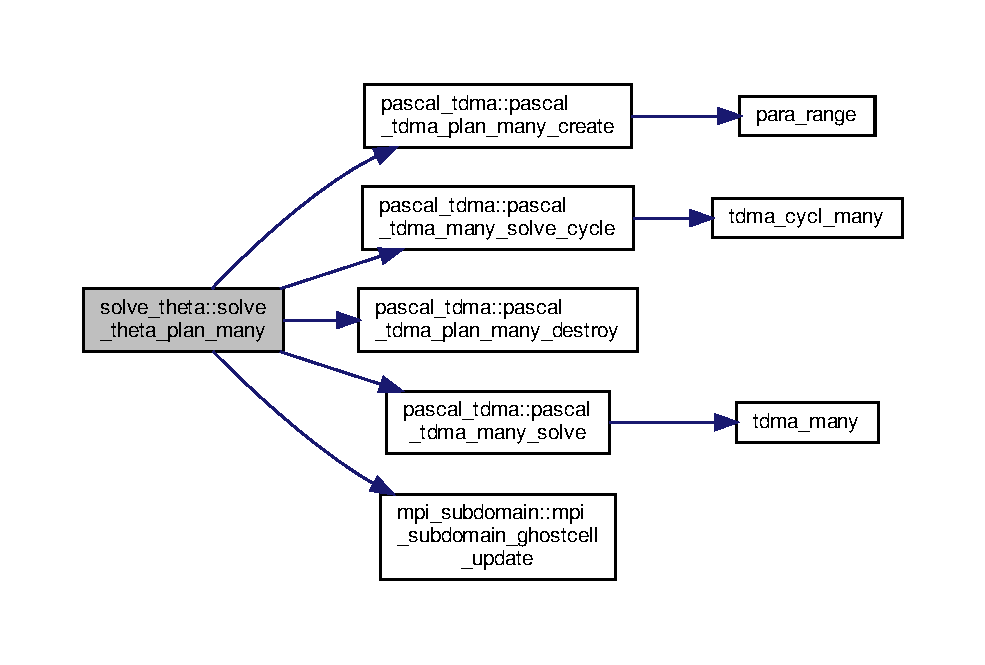
\includegraphics[width=350pt]{namespacesolve__theta_a0b7fdb576c007dc344092bf40efb0f4b_cgraph}
\end{center}
\end{figure}
\mbox{\Hypertarget{namespacesolve__theta_a84c4bdc671112259790470f6ad4c7e4c}\label{namespacesolve__theta_a84c4bdc671112259790470f6ad4c7e4c}} 
\index{solve\+\_\+theta@{solve\+\_\+theta}!solve\+\_\+theta\+\_\+plan\+\_\+many\+\_\+cuda@{solve\+\_\+theta\+\_\+plan\+\_\+many\+\_\+cuda}}
\index{solve\+\_\+theta\+\_\+plan\+\_\+many\+\_\+cuda@{solve\+\_\+theta\+\_\+plan\+\_\+many\+\_\+cuda}!solve\+\_\+theta@{solve\+\_\+theta}}
\subsubsection{\texorpdfstring{solve\+\_\+theta\+\_\+plan\+\_\+many\+\_\+cuda()}{solve\_theta\_plan\_many\_cuda()}}
{\footnotesize\ttfamily subroutine, public solve\+\_\+theta\+::solve\+\_\+theta\+\_\+plan\+\_\+many\+\_\+cuda (\begin{DoxyParamCaption}\item[{double precision, dimension(0\+:nx\+\_\+sub, 0\+:ny\+\_\+sub, 0\+:nz\+\_\+sub), intent(inout)}]{theta }\end{DoxyParamCaption})}



An example solver for many tridiagonal systems of equations using Pa\+Sca\+L\+\_\+\+T\+D\+MA with C\+U\+DA. 

This subroutine is for many tridiagonal systems of equations. It solves the the three-\/dimensional time-\/dependent heat conduction problem using Pa\+Sca\+L\+\_\+\+T\+D\+MA. Pa\+Sca\+L\+\_\+\+T\+D\+MA plans are created for many tridiagonal systems of equations and the many tridiagonal systems are solved plane-\/by-\/plane. 
\begin{DoxyParams}{Parameters}
{\em theta} & Main 3-\/D variable to be solved \\
\hline
\end{DoxyParams}
Here is the call graph for this function\+:
\nopagebreak
\begin{figure}[H]
\begin{center}
\leavevmode
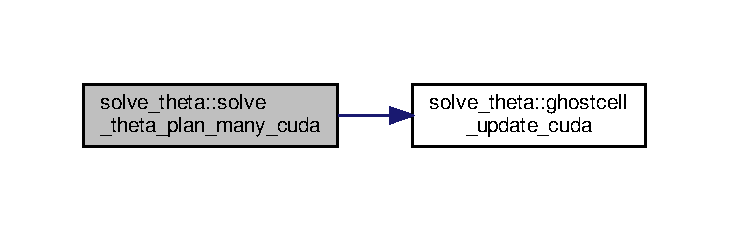
\includegraphics[width=350pt]{namespacesolve__theta_a84c4bdc671112259790470f6ad4c7e4c_cgraph}
\end{center}
\end{figure}
Here is the caller graph for this function\+:
\nopagebreak
\begin{figure}[H]
\begin{center}
\leavevmode
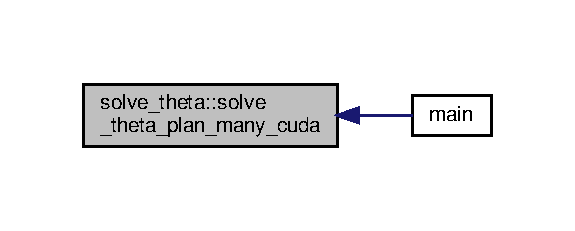
\includegraphics[width=276pt]{namespacesolve__theta_a84c4bdc671112259790470f6ad4c7e4c_icgraph}
\end{center}
\end{figure}
\mbox{\Hypertarget{namespacesolve__theta_a215d44e312ec3ab2a3ab44fa0613b100}\label{namespacesolve__theta_a215d44e312ec3ab2a3ab44fa0613b100}} 
\index{solve\+\_\+theta@{solve\+\_\+theta}!solve\+\_\+theta\+\_\+plan\+\_\+single@{solve\+\_\+theta\+\_\+plan\+\_\+single}}
\index{solve\+\_\+theta\+\_\+plan\+\_\+single@{solve\+\_\+theta\+\_\+plan\+\_\+single}!solve\+\_\+theta@{solve\+\_\+theta}}
\subsubsection{\texorpdfstring{solve\+\_\+theta\+\_\+plan\+\_\+single()}{solve\_theta\_plan\_single()}}
{\footnotesize\ttfamily subroutine, public solve\+\_\+theta\+::solve\+\_\+theta\+\_\+plan\+\_\+single (\begin{DoxyParamCaption}\item[{double precision, dimension(0\+:nx\+\_\+sub, 0\+:ny\+\_\+sub, 0\+:nz\+\_\+sub), intent(inout)}]{theta }\end{DoxyParamCaption})}



An example solver for a single tridiagonal system of equations using Pa\+Sca\+L\+\_\+\+T\+D\+MA. 

This subroutine is for a single tridiagonal system of equations. It solves the three-\/dimensional time-\/dependent heat conduction problem using Pa\+Sca\+L\+\_\+\+T\+D\+MA solver. Pa\+Sca\+L\+\_\+\+T\+D\+MA plans are created for a single tridiagonal system of equations and a single tridiagonal systems is solved line-\/by-\/line. 
\begin{DoxyParams}{Parameters}
{\em theta} & Main 3-\/D variable to be solved \\
\hline
\end{DoxyParams}
Here is the call graph for this function\+:
\nopagebreak
\begin{figure}[H]
\begin{center}
\leavevmode
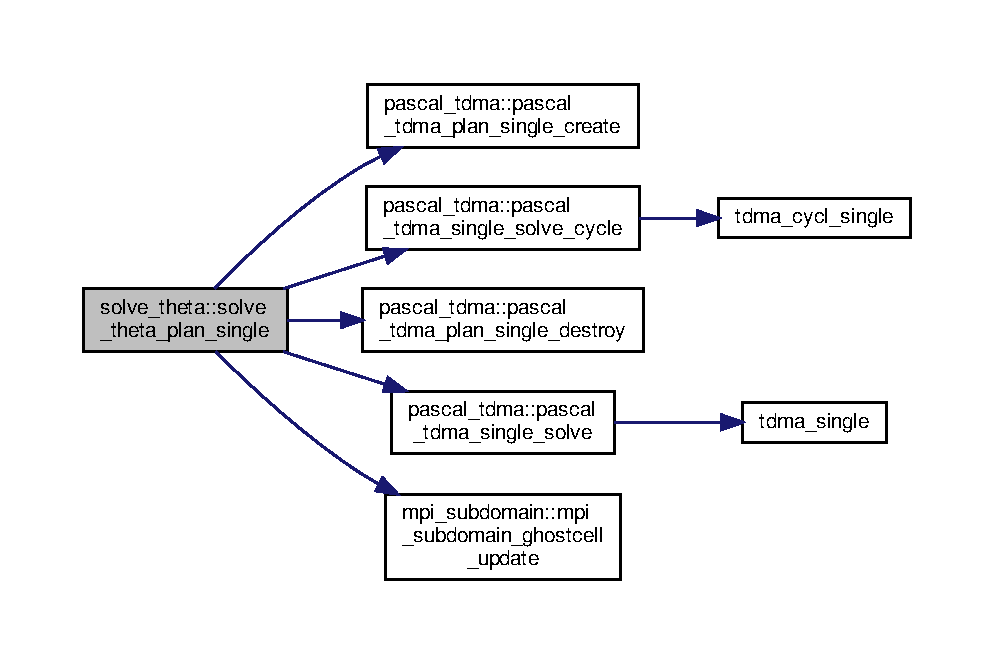
\includegraphics[width=350pt]{namespacesolve__theta_a215d44e312ec3ab2a3ab44fa0613b100_cgraph}
\end{center}
\end{figure}

\hypertarget{namespacetdma}{}\section{tdma Module Reference}
\label{namespacetdma}\index{tdma@{tdma}}

\chapter{Data Type Documentation}
\hypertarget{structmpi__topology_1_1cart__comm__1d}{}\section{mpi\+\_\+topology\+:\+:cart\+\_\+comm\+\_\+1d Type Reference}
\label{structmpi__topology_1_1cart__comm__1d}\index{mpi\+\_\+topology\+::cart\+\_\+comm\+\_\+1d@{mpi\+\_\+topology\+::cart\+\_\+comm\+\_\+1d}}


Type variable for the information of 1D communicator.  


\subsection*{Public Attributes}
\begin{DoxyCompactItemize}
\item 
integer \hyperlink{structmpi__topology_1_1cart__comm__1d_a0b76696fcf5c27f5cfdc48e53a2671ef}{myrank}
\begin{DoxyCompactList}\small\item\em Rank ID in current communicator. \end{DoxyCompactList}\item 
integer \hyperlink{structmpi__topology_1_1cart__comm__1d_adf78d1be6ca59cada6cc444edde4c3fc}{nprocs}
\begin{DoxyCompactList}\small\item\em Number of processes in current communicator. \end{DoxyCompactList}\item 
integer \hyperlink{structmpi__topology_1_1cart__comm__1d_a63baa1f74126ffda0b67af1c487dcd45}{west\+\_\+rank}
\begin{DoxyCompactList}\small\item\em Previous rank ID in current communicator. \end{DoxyCompactList}\item 
integer \hyperlink{structmpi__topology_1_1cart__comm__1d_a550b10f02ed0c5a8469174df8b54f525}{east\+\_\+rank}
\begin{DoxyCompactList}\small\item\em Next rank ID in current communicator. \end{DoxyCompactList}\item 
integer \hyperlink{structmpi__topology_1_1cart__comm__1d_ab9d9b0c2f72db4fb74c0264691778a45}{mpi\+\_\+comm}
\begin{DoxyCompactList}\small\item\em Current communicator. \end{DoxyCompactList}\end{DoxyCompactItemize}


\subsection{Detailed Description}
Type variable for the information of 1D communicator. 

\subsection{Member Data Documentation}
\mbox{\Hypertarget{structmpi__topology_1_1cart__comm__1d_a550b10f02ed0c5a8469174df8b54f525}\label{structmpi__topology_1_1cart__comm__1d_a550b10f02ed0c5a8469174df8b54f525}} 
\index{mpi\+\_\+topology\+::cart\+\_\+comm\+\_\+1d@{mpi\+\_\+topology\+::cart\+\_\+comm\+\_\+1d}!east\+\_\+rank@{east\+\_\+rank}}
\index{east\+\_\+rank@{east\+\_\+rank}!mpi\+\_\+topology\+::cart\+\_\+comm\+\_\+1d@{mpi\+\_\+topology\+::cart\+\_\+comm\+\_\+1d}}
\subsubsection{\texorpdfstring{east\+\_\+rank}{east\_rank}}
{\footnotesize\ttfamily integer mpi\+\_\+topology\+::cart\+\_\+comm\+\_\+1d\+::east\+\_\+rank}



Next rank ID in current communicator. 

\mbox{\Hypertarget{structmpi__topology_1_1cart__comm__1d_ab9d9b0c2f72db4fb74c0264691778a45}\label{structmpi__topology_1_1cart__comm__1d_ab9d9b0c2f72db4fb74c0264691778a45}} 
\index{mpi\+\_\+topology\+::cart\+\_\+comm\+\_\+1d@{mpi\+\_\+topology\+::cart\+\_\+comm\+\_\+1d}!mpi\+\_\+comm@{mpi\+\_\+comm}}
\index{mpi\+\_\+comm@{mpi\+\_\+comm}!mpi\+\_\+topology\+::cart\+\_\+comm\+\_\+1d@{mpi\+\_\+topology\+::cart\+\_\+comm\+\_\+1d}}
\subsubsection{\texorpdfstring{mpi\+\_\+comm}{mpi\_comm}}
{\footnotesize\ttfamily integer mpi\+\_\+topology\+::cart\+\_\+comm\+\_\+1d\+::mpi\+\_\+comm}



Current communicator. 

\mbox{\Hypertarget{structmpi__topology_1_1cart__comm__1d_a0b76696fcf5c27f5cfdc48e53a2671ef}\label{structmpi__topology_1_1cart__comm__1d_a0b76696fcf5c27f5cfdc48e53a2671ef}} 
\index{mpi\+\_\+topology\+::cart\+\_\+comm\+\_\+1d@{mpi\+\_\+topology\+::cart\+\_\+comm\+\_\+1d}!myrank@{myrank}}
\index{myrank@{myrank}!mpi\+\_\+topology\+::cart\+\_\+comm\+\_\+1d@{mpi\+\_\+topology\+::cart\+\_\+comm\+\_\+1d}}
\subsubsection{\texorpdfstring{myrank}{myrank}}
{\footnotesize\ttfamily integer mpi\+\_\+topology\+::cart\+\_\+comm\+\_\+1d\+::myrank}



Rank ID in current communicator. 

\mbox{\Hypertarget{structmpi__topology_1_1cart__comm__1d_adf78d1be6ca59cada6cc444edde4c3fc}\label{structmpi__topology_1_1cart__comm__1d_adf78d1be6ca59cada6cc444edde4c3fc}} 
\index{mpi\+\_\+topology\+::cart\+\_\+comm\+\_\+1d@{mpi\+\_\+topology\+::cart\+\_\+comm\+\_\+1d}!nprocs@{nprocs}}
\index{nprocs@{nprocs}!mpi\+\_\+topology\+::cart\+\_\+comm\+\_\+1d@{mpi\+\_\+topology\+::cart\+\_\+comm\+\_\+1d}}
\subsubsection{\texorpdfstring{nprocs}{nprocs}}
{\footnotesize\ttfamily integer mpi\+\_\+topology\+::cart\+\_\+comm\+\_\+1d\+::nprocs}



Number of processes in current communicator. 

\mbox{\Hypertarget{structmpi__topology_1_1cart__comm__1d_a63baa1f74126ffda0b67af1c487dcd45}\label{structmpi__topology_1_1cart__comm__1d_a63baa1f74126ffda0b67af1c487dcd45}} 
\index{mpi\+\_\+topology\+::cart\+\_\+comm\+\_\+1d@{mpi\+\_\+topology\+::cart\+\_\+comm\+\_\+1d}!west\+\_\+rank@{west\+\_\+rank}}
\index{west\+\_\+rank@{west\+\_\+rank}!mpi\+\_\+topology\+::cart\+\_\+comm\+\_\+1d@{mpi\+\_\+topology\+::cart\+\_\+comm\+\_\+1d}}
\subsubsection{\texorpdfstring{west\+\_\+rank}{west\_rank}}
{\footnotesize\ttfamily integer mpi\+\_\+topology\+::cart\+\_\+comm\+\_\+1d\+::west\+\_\+rank}



Previous rank ID in current communicator. 



The documentation for this type was generated from the following file\+:\begin{DoxyCompactItemize}
\item 
/home/jihoon/\+Develop/\+Pa\+Sca\+L\+\_\+\+T\+D\+M\+A/examples/\hyperlink{mpi__topology_8f90}{mpi\+\_\+topology.\+f90}\end{DoxyCompactItemize}

\hypertarget{structnvtx_1_1nvtxeventattributes}{}\section{nvtx\+:\+:nvtxeventattributes Type Reference}
\label{structnvtx_1_1nvtxeventattributes}\index{nvtx\+::nvtxeventattributes@{nvtx\+::nvtxeventattributes}}
\subsection*{Public Attributes}
\begin{DoxyCompactItemize}
\item 
integer(c\+\_\+int16\+\_\+t) \hyperlink{structnvtx_1_1nvtxeventattributes_a3e1c1186627d3585041f5107f7a2c6cf}{version} =1
\item 
integer(c\+\_\+int16\+\_\+t) \hyperlink{structnvtx_1_1nvtxeventattributes_a073c788ac024351d153f5fa2a54a03dc}{size} =48
\item 
integer(c\+\_\+int) \hyperlink{structnvtx_1_1nvtxeventattributes_a76a24ba48d19336d353e253605ec177a}{category} =0
\item 
integer(c\+\_\+int) \hyperlink{structnvtx_1_1nvtxeventattributes_a31a68afdd45c9dbc5b60759d6a43da80}{colortype} =1
\item 
integer(c\+\_\+int) \hyperlink{structnvtx_1_1nvtxeventattributes_a77bb01e48bd71036991bf1232f5e4dd0}{color}
\item 
integer(c\+\_\+int) \hyperlink{structnvtx_1_1nvtxeventattributes_a5c6946881915f624b3080b708501bf74}{payloadtype} =0
\item 
integer(c\+\_\+int) \hyperlink{structnvtx_1_1nvtxeventattributes_aa109ecc1e38adcbf2b52661ed72e6286}{reserved0}
\item 
integer(c\+\_\+int64\+\_\+t) \hyperlink{structnvtx_1_1nvtxeventattributes_a4f3974f0da3b572f86b0358c46a5e09b}{payload}
\item 
integer(c\+\_\+int) \hyperlink{structnvtx_1_1nvtxeventattributes_af2fd0cfacc31da95db6a9037ace4bcdc}{messagetype} =1
\item 
type(c\+\_\+ptr) \hyperlink{structnvtx_1_1nvtxeventattributes_a988faa8b845122161036f87fe2034ee1}{message}
\end{DoxyCompactItemize}


\subsection{Member Data Documentation}
\mbox{\Hypertarget{structnvtx_1_1nvtxeventattributes_a76a24ba48d19336d353e253605ec177a}\label{structnvtx_1_1nvtxeventattributes_a76a24ba48d19336d353e253605ec177a}} 
\index{nvtx\+::nvtxeventattributes@{nvtx\+::nvtxeventattributes}!category@{category}}
\index{category@{category}!nvtx\+::nvtxeventattributes@{nvtx\+::nvtxeventattributes}}
\subsubsection{\texorpdfstring{category}{category}}
{\footnotesize\ttfamily integer(c\+\_\+int) nvtx\+::nvtxeventattributes\+::category =0}

\mbox{\Hypertarget{structnvtx_1_1nvtxeventattributes_a77bb01e48bd71036991bf1232f5e4dd0}\label{structnvtx_1_1nvtxeventattributes_a77bb01e48bd71036991bf1232f5e4dd0}} 
\index{nvtx\+::nvtxeventattributes@{nvtx\+::nvtxeventattributes}!color@{color}}
\index{color@{color}!nvtx\+::nvtxeventattributes@{nvtx\+::nvtxeventattributes}}
\subsubsection{\texorpdfstring{color}{color}}
{\footnotesize\ttfamily integer(c\+\_\+int) nvtx\+::nvtxeventattributes\+::color}

\mbox{\Hypertarget{structnvtx_1_1nvtxeventattributes_a31a68afdd45c9dbc5b60759d6a43da80}\label{structnvtx_1_1nvtxeventattributes_a31a68afdd45c9dbc5b60759d6a43da80}} 
\index{nvtx\+::nvtxeventattributes@{nvtx\+::nvtxeventattributes}!colortype@{colortype}}
\index{colortype@{colortype}!nvtx\+::nvtxeventattributes@{nvtx\+::nvtxeventattributes}}
\subsubsection{\texorpdfstring{colortype}{colortype}}
{\footnotesize\ttfamily integer(c\+\_\+int) nvtx\+::nvtxeventattributes\+::colortype =1}

\mbox{\Hypertarget{structnvtx_1_1nvtxeventattributes_a988faa8b845122161036f87fe2034ee1}\label{structnvtx_1_1nvtxeventattributes_a988faa8b845122161036f87fe2034ee1}} 
\index{nvtx\+::nvtxeventattributes@{nvtx\+::nvtxeventattributes}!message@{message}}
\index{message@{message}!nvtx\+::nvtxeventattributes@{nvtx\+::nvtxeventattributes}}
\subsubsection{\texorpdfstring{message}{message}}
{\footnotesize\ttfamily type(c\+\_\+ptr) nvtx\+::nvtxeventattributes\+::message}

\mbox{\Hypertarget{structnvtx_1_1nvtxeventattributes_af2fd0cfacc31da95db6a9037ace4bcdc}\label{structnvtx_1_1nvtxeventattributes_af2fd0cfacc31da95db6a9037ace4bcdc}} 
\index{nvtx\+::nvtxeventattributes@{nvtx\+::nvtxeventattributes}!messagetype@{messagetype}}
\index{messagetype@{messagetype}!nvtx\+::nvtxeventattributes@{nvtx\+::nvtxeventattributes}}
\subsubsection{\texorpdfstring{messagetype}{messagetype}}
{\footnotesize\ttfamily integer(c\+\_\+int) nvtx\+::nvtxeventattributes\+::messagetype =1}

\mbox{\Hypertarget{structnvtx_1_1nvtxeventattributes_a4f3974f0da3b572f86b0358c46a5e09b}\label{structnvtx_1_1nvtxeventattributes_a4f3974f0da3b572f86b0358c46a5e09b}} 
\index{nvtx\+::nvtxeventattributes@{nvtx\+::nvtxeventattributes}!payload@{payload}}
\index{payload@{payload}!nvtx\+::nvtxeventattributes@{nvtx\+::nvtxeventattributes}}
\subsubsection{\texorpdfstring{payload}{payload}}
{\footnotesize\ttfamily integer(c\+\_\+int64\+\_\+t) nvtx\+::nvtxeventattributes\+::payload}

\mbox{\Hypertarget{structnvtx_1_1nvtxeventattributes_a5c6946881915f624b3080b708501bf74}\label{structnvtx_1_1nvtxeventattributes_a5c6946881915f624b3080b708501bf74}} 
\index{nvtx\+::nvtxeventattributes@{nvtx\+::nvtxeventattributes}!payloadtype@{payloadtype}}
\index{payloadtype@{payloadtype}!nvtx\+::nvtxeventattributes@{nvtx\+::nvtxeventattributes}}
\subsubsection{\texorpdfstring{payloadtype}{payloadtype}}
{\footnotesize\ttfamily integer(c\+\_\+int) nvtx\+::nvtxeventattributes\+::payloadtype =0}

\mbox{\Hypertarget{structnvtx_1_1nvtxeventattributes_aa109ecc1e38adcbf2b52661ed72e6286}\label{structnvtx_1_1nvtxeventattributes_aa109ecc1e38adcbf2b52661ed72e6286}} 
\index{nvtx\+::nvtxeventattributes@{nvtx\+::nvtxeventattributes}!reserved0@{reserved0}}
\index{reserved0@{reserved0}!nvtx\+::nvtxeventattributes@{nvtx\+::nvtxeventattributes}}
\subsubsection{\texorpdfstring{reserved0}{reserved0}}
{\footnotesize\ttfamily integer(c\+\_\+int) nvtx\+::nvtxeventattributes\+::reserved0}

\mbox{\Hypertarget{structnvtx_1_1nvtxeventattributes_a073c788ac024351d153f5fa2a54a03dc}\label{structnvtx_1_1nvtxeventattributes_a073c788ac024351d153f5fa2a54a03dc}} 
\index{nvtx\+::nvtxeventattributes@{nvtx\+::nvtxeventattributes}!size@{size}}
\index{size@{size}!nvtx\+::nvtxeventattributes@{nvtx\+::nvtxeventattributes}}
\subsubsection{\texorpdfstring{size}{size}}
{\footnotesize\ttfamily integer(c\+\_\+int16\+\_\+t) nvtx\+::nvtxeventattributes\+::size =48}

\mbox{\Hypertarget{structnvtx_1_1nvtxeventattributes_a3e1c1186627d3585041f5107f7a2c6cf}\label{structnvtx_1_1nvtxeventattributes_a3e1c1186627d3585041f5107f7a2c6cf}} 
\index{nvtx\+::nvtxeventattributes@{nvtx\+::nvtxeventattributes}!version@{version}}
\index{version@{version}!nvtx\+::nvtxeventattributes@{nvtx\+::nvtxeventattributes}}
\subsubsection{\texorpdfstring{version}{version}}
{\footnotesize\ttfamily integer(c\+\_\+int16\+\_\+t) nvtx\+::nvtxeventattributes\+::version =1}



The documentation for this type was generated from the following file\+:\begin{DoxyCompactItemize}
\item 
/home/jihoon/\+Develop/\+Pa\+Sca\+L\+\_\+\+T\+D\+M\+A/src/\hyperlink{nvtx_8f90}{nvtx.\+f90}\end{DoxyCompactItemize}

\hypertarget{interfacenvtx_1_1nvtxrangepop}{}\section{nvtx\+:\+:nvtxrangepop Interface Reference}
\label{interfacenvtx_1_1nvtxrangepop}\index{nvtx\+::nvtxrangepop@{nvtx\+::nvtxrangepop}}
\subsection*{Public Member Functions}
\begin{DoxyCompactItemize}
\item 
subroutine \hyperlink{interfacenvtx_1_1nvtxrangepop_ade36ac9b48a28449dab91510ce6e4a02}{nvtxrangepop} ()
\end{DoxyCompactItemize}


\subsection{Constructor \& Destructor Documentation}
\mbox{\Hypertarget{interfacenvtx_1_1nvtxrangepop_ade36ac9b48a28449dab91510ce6e4a02}\label{interfacenvtx_1_1nvtxrangepop_ade36ac9b48a28449dab91510ce6e4a02}} 
\index{nvtx\+::nvtxrangepop@{nvtx\+::nvtxrangepop}!nvtxrangepop@{nvtxrangepop}}
\index{nvtxrangepop@{nvtxrangepop}!nvtx\+::nvtxrangepop@{nvtx\+::nvtxrangepop}}
\subsubsection{\texorpdfstring{nvtxrangepop()}{nvtxrangepop()}}
{\footnotesize\ttfamily subroutine nvtx\+::nvtxrangepop\+::nvtxrangepop (\begin{DoxyParamCaption}{ }\end{DoxyParamCaption})}



The documentation for this interface was generated from the following file\+:\begin{DoxyCompactItemize}
\item 
/home/jihoon/\+Develop/\+Pa\+Sca\+L\+\_\+\+T\+D\+M\+A/src/\hyperlink{nvtx_8f90}{nvtx.\+f90}\end{DoxyCompactItemize}

\hypertarget{interfacenvtx_1_1nvtxrangepush}{}\section{nvtx\+:\+:nvtxrangepush Interface Reference}
\label{interfacenvtx_1_1nvtxrangepush}\index{nvtx\+::nvtxrangepush@{nvtx\+::nvtxrangepush}}
\subsection*{Public Member Functions}
\begin{DoxyCompactItemize}
\item 
subroutine \hyperlink{interfacenvtx_1_1nvtxrangepush_a9b89d40371882183ffd7f3c6afb7c32a}{nvtxrangepusha} (name)
\item 
subroutine \hyperlink{interfacenvtx_1_1nvtxrangepush_ab940fa7d62630e799d93f4a6bbe64fd7}{nvtxrangepushex} (event)
\end{DoxyCompactItemize}


\subsection{Member Function/\+Subroutine Documentation}
\mbox{\Hypertarget{interfacenvtx_1_1nvtxrangepush_a9b89d40371882183ffd7f3c6afb7c32a}\label{interfacenvtx_1_1nvtxrangepush_a9b89d40371882183ffd7f3c6afb7c32a}} 
\index{nvtx\+::nvtxrangepush@{nvtx\+::nvtxrangepush}!nvtxrangepusha@{nvtxrangepusha}}
\index{nvtxrangepusha@{nvtxrangepusha}!nvtx\+::nvtxrangepush@{nvtx\+::nvtxrangepush}}
\subsubsection{\texorpdfstring{nvtxrangepusha()}{nvtxrangepusha()}}
{\footnotesize\ttfamily subroutine nvtx\+::nvtxrangepush\+::nvtxrangepusha (\begin{DoxyParamCaption}\item[{character(kind=c\+\_\+char), dimension(256)}]{name }\end{DoxyParamCaption})}

\mbox{\Hypertarget{interfacenvtx_1_1nvtxrangepush_ab940fa7d62630e799d93f4a6bbe64fd7}\label{interfacenvtx_1_1nvtxrangepush_ab940fa7d62630e799d93f4a6bbe64fd7}} 
\index{nvtx\+::nvtxrangepush@{nvtx\+::nvtxrangepush}!nvtxrangepushex@{nvtxrangepushex}}
\index{nvtxrangepushex@{nvtxrangepushex}!nvtx\+::nvtxrangepush@{nvtx\+::nvtxrangepush}}
\subsubsection{\texorpdfstring{nvtxrangepushex()}{nvtxrangepushex()}}
{\footnotesize\ttfamily subroutine nvtx\+::nvtxrangepush\+::nvtxrangepushex (\begin{DoxyParamCaption}\item[{type(\hyperlink{structnvtx_1_1nvtxeventattributes}{nvtxeventattributes})}]{event }\end{DoxyParamCaption})}



The documentation for this interface was generated from the following file\+:\begin{DoxyCompactItemize}
\item 
/home/jihoon/\+Develop/\+Pa\+Sca\+L\+\_\+\+T\+D\+M\+A/src/\hyperlink{nvtx_8f90}{nvtx.\+f90}\end{DoxyCompactItemize}

\hypertarget{structpascal__tdma_1_1ptdma__plan__many}{}\section{pascal\+\_\+tdma\+:\+:ptdma\+\_\+plan\+\_\+many Type Reference}
\label{structpascal__tdma_1_1ptdma__plan__many}\index{pascal\+\_\+tdma\+::ptdma\+\_\+plan\+\_\+many@{pascal\+\_\+tdma\+::ptdma\+\_\+plan\+\_\+many}}


Execution plan for many tridiagonal systems of equations.  


\subsection*{Public Attributes}
\begin{DoxyCompactItemize}
\item 
integer \hyperlink{structpascal__tdma_1_1ptdma__plan__many_acb7e645e37c791564905c6e2808db0c6}{ptdma\+\_\+world}
\begin{DoxyCompactList}\small\item\em Single dimensional subcommunicator to assemble data for the reduced T\+D\+MA. \end{DoxyCompactList}\item 
integer \hyperlink{structpascal__tdma_1_1ptdma__plan__many_a22b42947ab742f83aad3bbeb3a42a0f6}{n\+\_\+sys\+\_\+rt}
\begin{DoxyCompactList}\small\item\em Number of tridiagonal systems that need to be solved in each process after transpose. \end{DoxyCompactList}\item 
integer \hyperlink{structpascal__tdma_1_1ptdma__plan__many_ad94248e2aa0653f151f0575d62d6fff7}{n\+\_\+row\+\_\+rt}
\begin{DoxyCompactList}\small\item\em Number of rows of a reduced tridiagonal systems after transpose. \end{DoxyCompactList}\item 
integer \hyperlink{structpascal__tdma_1_1ptdma__plan__many_aefad054b588906989c2fdfc5ef9cb6d4}{nprocs}
\begin{DoxyCompactList}\small\item\em Communicator size of ptdma\+\_\+world. \end{DoxyCompactList}\end{DoxyCompactItemize}
\textbf{ }\par
\begin{DoxyCompactItemize}
\item 
integer, dimension(\+:), allocatable \hyperlink{structpascal__tdma_1_1ptdma__plan__many_ad95f6ed58387dd66baecf53ed5fab7e8}{ddtype\+\_\+fs}
\begin{DoxyCompactList}\small\item\em Send buffer related variables for M\+P\+I\+\_\+\+Ialltoallw. \end{DoxyCompactList}\item 
integer, dimension(\+:), allocatable \hyperlink{structpascal__tdma_1_1ptdma__plan__many_ab7a5a4be85650cfe4dfc30fd83b132d7}{count\+\_\+send}
\item 
integer, dimension(\+:), allocatable \hyperlink{structpascal__tdma_1_1ptdma__plan__many_a1c7544758e7ccfcd3b07e91caf0d8f3d}{displ\+\_\+send}
\end{DoxyCompactItemize}

\textbf{ }\par
\begin{DoxyCompactItemize}
\item 
integer, dimension(\+:), allocatable \hyperlink{structpascal__tdma_1_1ptdma__plan__many_a54ddb10078b443daf47204cdcd8e7f8f}{ddtype\+\_\+bs}
\begin{DoxyCompactList}\small\item\em Recv. buffer related variables M\+P\+I\+\_\+\+Ialltoallw. \end{DoxyCompactList}\item 
integer, dimension(\+:), allocatable \hyperlink{structpascal__tdma_1_1ptdma__plan__many_a30cebfb14bfcc955d3e98d9b1ea5fad7}{count\+\_\+recv}
\item 
integer, dimension(\+:), allocatable \hyperlink{structpascal__tdma_1_1ptdma__plan__many_a1801ea6bbff319dd594a5e993bc5d542}{displ\+\_\+recv}
\end{DoxyCompactItemize}

\textbf{ }\par
\begin{DoxyCompactItemize}
\item 
double precision, dimension(\+:,\+:), allocatable \hyperlink{structpascal__tdma_1_1ptdma__plan__many_a6d9101716eca623dc8c45075788f06bd}{a\+\_\+rd}
\begin{DoxyCompactList}\small\item\em Coefficient arrays after reduction, a\+: lower, b\+: diagonal, c\+: upper, d\+: rhs. The orginal dimension (m\+:n) is reduced to (m\+:2) \end{DoxyCompactList}\item 
double precision, dimension(\+:,\+:), allocatable \hyperlink{structpascal__tdma_1_1ptdma__plan__many_a81ed1b6910c30334e93598f7d18254a3}{b\+\_\+rd}
\item 
double precision, dimension(\+:,\+:), allocatable \hyperlink{structpascal__tdma_1_1ptdma__plan__many_a56b15fe2b742c06106a46da7a720d9fd}{c\+\_\+rd}
\item 
double precision, dimension(\+:,\+:), allocatable \hyperlink{structpascal__tdma_1_1ptdma__plan__many_aa1054814f874504a77ad17a838a80fd2}{d\+\_\+rd}
\end{DoxyCompactItemize}

\textbf{ }\par
\begin{DoxyCompactItemize}
\item 
double precision, dimension(\+:,\+:), allocatable \hyperlink{structpascal__tdma_1_1ptdma__plan__many_a42be039aee75c5393c22111cf232e77d}{a\+\_\+rt}
\begin{DoxyCompactList}\small\item\em Coefficient arrays after transpose of reduced systems, a\+: lower, b\+: diagonal, c\+: upper, d\+: rhs The reduced dimension (m\+:2) changes to (m/np\+: 2$\ast$np) after transpose. \end{DoxyCompactList}\item 
double precision, dimension(\+:,\+:), allocatable \hyperlink{structpascal__tdma_1_1ptdma__plan__many_aab84eff7c823d47acb5388cd4e2a790a}{b\+\_\+rt}
\item 
double precision, dimension(\+:,\+:), allocatable \hyperlink{structpascal__tdma_1_1ptdma__plan__many_a49336d53d19c274798e87ae33b530b33}{c\+\_\+rt}
\item 
double precision, dimension(\+:,\+:), allocatable \hyperlink{structpascal__tdma_1_1ptdma__plan__many_af0941ce4b9206c36a3a059d2bae84d2b}{d\+\_\+rt}
\end{DoxyCompactItemize}



\subsection{Detailed Description}
Execution plan for many tridiagonal systems of equations. 

It uses M\+P\+I\+\_\+\+Ialltoallw function to distribute the modified tridiagonal systems to M\+PI processes and build the reduced tridiagonal systems of equations. Derived datatypes are defined and used to eliminate the cost of data packing and unpacking. 

\subsection{Member Data Documentation}
\mbox{\Hypertarget{structpascal__tdma_1_1ptdma__plan__many_a6d9101716eca623dc8c45075788f06bd}\label{structpascal__tdma_1_1ptdma__plan__many_a6d9101716eca623dc8c45075788f06bd}} 
\index{pascal\+\_\+tdma\+::ptdma\+\_\+plan\+\_\+many@{pascal\+\_\+tdma\+::ptdma\+\_\+plan\+\_\+many}!a\+\_\+rd@{a\+\_\+rd}}
\index{a\+\_\+rd@{a\+\_\+rd}!pascal\+\_\+tdma\+::ptdma\+\_\+plan\+\_\+many@{pascal\+\_\+tdma\+::ptdma\+\_\+plan\+\_\+many}}
\subsubsection{\texorpdfstring{a\+\_\+rd}{a\_rd}}
{\footnotesize\ttfamily double precision, dimension(\+:,\+:), allocatable pascal\+\_\+tdma\+::ptdma\+\_\+plan\+\_\+many\+::a\+\_\+rd}



Coefficient arrays after reduction, a\+: lower, b\+: diagonal, c\+: upper, d\+: rhs. The orginal dimension (m\+:n) is reduced to (m\+:2) 

\mbox{\Hypertarget{structpascal__tdma_1_1ptdma__plan__many_a42be039aee75c5393c22111cf232e77d}\label{structpascal__tdma_1_1ptdma__plan__many_a42be039aee75c5393c22111cf232e77d}} 
\index{pascal\+\_\+tdma\+::ptdma\+\_\+plan\+\_\+many@{pascal\+\_\+tdma\+::ptdma\+\_\+plan\+\_\+many}!a\+\_\+rt@{a\+\_\+rt}}
\index{a\+\_\+rt@{a\+\_\+rt}!pascal\+\_\+tdma\+::ptdma\+\_\+plan\+\_\+many@{pascal\+\_\+tdma\+::ptdma\+\_\+plan\+\_\+many}}
\subsubsection{\texorpdfstring{a\+\_\+rt}{a\_rt}}
{\footnotesize\ttfamily double precision, dimension(\+:,\+:), allocatable pascal\+\_\+tdma\+::ptdma\+\_\+plan\+\_\+many\+::a\+\_\+rt}



Coefficient arrays after transpose of reduced systems, a\+: lower, b\+: diagonal, c\+: upper, d\+: rhs The reduced dimension (m\+:2) changes to (m/np\+: 2$\ast$np) after transpose. 

\mbox{\Hypertarget{structpascal__tdma_1_1ptdma__plan__many_a81ed1b6910c30334e93598f7d18254a3}\label{structpascal__tdma_1_1ptdma__plan__many_a81ed1b6910c30334e93598f7d18254a3}} 
\index{pascal\+\_\+tdma\+::ptdma\+\_\+plan\+\_\+many@{pascal\+\_\+tdma\+::ptdma\+\_\+plan\+\_\+many}!b\+\_\+rd@{b\+\_\+rd}}
\index{b\+\_\+rd@{b\+\_\+rd}!pascal\+\_\+tdma\+::ptdma\+\_\+plan\+\_\+many@{pascal\+\_\+tdma\+::ptdma\+\_\+plan\+\_\+many}}
\subsubsection{\texorpdfstring{b\+\_\+rd}{b\_rd}}
{\footnotesize\ttfamily double precision, dimension(\+:,\+:), allocatable pascal\+\_\+tdma\+::ptdma\+\_\+plan\+\_\+many\+::b\+\_\+rd}

\mbox{\Hypertarget{structpascal__tdma_1_1ptdma__plan__many_aab84eff7c823d47acb5388cd4e2a790a}\label{structpascal__tdma_1_1ptdma__plan__many_aab84eff7c823d47acb5388cd4e2a790a}} 
\index{pascal\+\_\+tdma\+::ptdma\+\_\+plan\+\_\+many@{pascal\+\_\+tdma\+::ptdma\+\_\+plan\+\_\+many}!b\+\_\+rt@{b\+\_\+rt}}
\index{b\+\_\+rt@{b\+\_\+rt}!pascal\+\_\+tdma\+::ptdma\+\_\+plan\+\_\+many@{pascal\+\_\+tdma\+::ptdma\+\_\+plan\+\_\+many}}
\subsubsection{\texorpdfstring{b\+\_\+rt}{b\_rt}}
{\footnotesize\ttfamily double precision, dimension(\+:,\+:), allocatable pascal\+\_\+tdma\+::ptdma\+\_\+plan\+\_\+many\+::b\+\_\+rt}

\mbox{\Hypertarget{structpascal__tdma_1_1ptdma__plan__many_a56b15fe2b742c06106a46da7a720d9fd}\label{structpascal__tdma_1_1ptdma__plan__many_a56b15fe2b742c06106a46da7a720d9fd}} 
\index{pascal\+\_\+tdma\+::ptdma\+\_\+plan\+\_\+many@{pascal\+\_\+tdma\+::ptdma\+\_\+plan\+\_\+many}!c\+\_\+rd@{c\+\_\+rd}}
\index{c\+\_\+rd@{c\+\_\+rd}!pascal\+\_\+tdma\+::ptdma\+\_\+plan\+\_\+many@{pascal\+\_\+tdma\+::ptdma\+\_\+plan\+\_\+many}}
\subsubsection{\texorpdfstring{c\+\_\+rd}{c\_rd}}
{\footnotesize\ttfamily double precision, dimension(\+:,\+:), allocatable pascal\+\_\+tdma\+::ptdma\+\_\+plan\+\_\+many\+::c\+\_\+rd}

\mbox{\Hypertarget{structpascal__tdma_1_1ptdma__plan__many_a49336d53d19c274798e87ae33b530b33}\label{structpascal__tdma_1_1ptdma__plan__many_a49336d53d19c274798e87ae33b530b33}} 
\index{pascal\+\_\+tdma\+::ptdma\+\_\+plan\+\_\+many@{pascal\+\_\+tdma\+::ptdma\+\_\+plan\+\_\+many}!c\+\_\+rt@{c\+\_\+rt}}
\index{c\+\_\+rt@{c\+\_\+rt}!pascal\+\_\+tdma\+::ptdma\+\_\+plan\+\_\+many@{pascal\+\_\+tdma\+::ptdma\+\_\+plan\+\_\+many}}
\subsubsection{\texorpdfstring{c\+\_\+rt}{c\_rt}}
{\footnotesize\ttfamily double precision, dimension(\+:,\+:), allocatable pascal\+\_\+tdma\+::ptdma\+\_\+plan\+\_\+many\+::c\+\_\+rt}

\mbox{\Hypertarget{structpascal__tdma_1_1ptdma__plan__many_a30cebfb14bfcc955d3e98d9b1ea5fad7}\label{structpascal__tdma_1_1ptdma__plan__many_a30cebfb14bfcc955d3e98d9b1ea5fad7}} 
\index{pascal\+\_\+tdma\+::ptdma\+\_\+plan\+\_\+many@{pascal\+\_\+tdma\+::ptdma\+\_\+plan\+\_\+many}!count\+\_\+recv@{count\+\_\+recv}}
\index{count\+\_\+recv@{count\+\_\+recv}!pascal\+\_\+tdma\+::ptdma\+\_\+plan\+\_\+many@{pascal\+\_\+tdma\+::ptdma\+\_\+plan\+\_\+many}}
\subsubsection{\texorpdfstring{count\+\_\+recv}{count\_recv}}
{\footnotesize\ttfamily integer, dimension(\+:), allocatable pascal\+\_\+tdma\+::ptdma\+\_\+plan\+\_\+many\+::count\+\_\+recv}

\mbox{\Hypertarget{structpascal__tdma_1_1ptdma__plan__many_ab7a5a4be85650cfe4dfc30fd83b132d7}\label{structpascal__tdma_1_1ptdma__plan__many_ab7a5a4be85650cfe4dfc30fd83b132d7}} 
\index{pascal\+\_\+tdma\+::ptdma\+\_\+plan\+\_\+many@{pascal\+\_\+tdma\+::ptdma\+\_\+plan\+\_\+many}!count\+\_\+send@{count\+\_\+send}}
\index{count\+\_\+send@{count\+\_\+send}!pascal\+\_\+tdma\+::ptdma\+\_\+plan\+\_\+many@{pascal\+\_\+tdma\+::ptdma\+\_\+plan\+\_\+many}}
\subsubsection{\texorpdfstring{count\+\_\+send}{count\_send}}
{\footnotesize\ttfamily integer, dimension(\+:), allocatable pascal\+\_\+tdma\+::ptdma\+\_\+plan\+\_\+many\+::count\+\_\+send}

\mbox{\Hypertarget{structpascal__tdma_1_1ptdma__plan__many_aa1054814f874504a77ad17a838a80fd2}\label{structpascal__tdma_1_1ptdma__plan__many_aa1054814f874504a77ad17a838a80fd2}} 
\index{pascal\+\_\+tdma\+::ptdma\+\_\+plan\+\_\+many@{pascal\+\_\+tdma\+::ptdma\+\_\+plan\+\_\+many}!d\+\_\+rd@{d\+\_\+rd}}
\index{d\+\_\+rd@{d\+\_\+rd}!pascal\+\_\+tdma\+::ptdma\+\_\+plan\+\_\+many@{pascal\+\_\+tdma\+::ptdma\+\_\+plan\+\_\+many}}
\subsubsection{\texorpdfstring{d\+\_\+rd}{d\_rd}}
{\footnotesize\ttfamily double precision, dimension(\+:,\+:), allocatable pascal\+\_\+tdma\+::ptdma\+\_\+plan\+\_\+many\+::d\+\_\+rd}

\mbox{\Hypertarget{structpascal__tdma_1_1ptdma__plan__many_af0941ce4b9206c36a3a059d2bae84d2b}\label{structpascal__tdma_1_1ptdma__plan__many_af0941ce4b9206c36a3a059d2bae84d2b}} 
\index{pascal\+\_\+tdma\+::ptdma\+\_\+plan\+\_\+many@{pascal\+\_\+tdma\+::ptdma\+\_\+plan\+\_\+many}!d\+\_\+rt@{d\+\_\+rt}}
\index{d\+\_\+rt@{d\+\_\+rt}!pascal\+\_\+tdma\+::ptdma\+\_\+plan\+\_\+many@{pascal\+\_\+tdma\+::ptdma\+\_\+plan\+\_\+many}}
\subsubsection{\texorpdfstring{d\+\_\+rt}{d\_rt}}
{\footnotesize\ttfamily double precision, dimension(\+:,\+:), allocatable pascal\+\_\+tdma\+::ptdma\+\_\+plan\+\_\+many\+::d\+\_\+rt}

\mbox{\Hypertarget{structpascal__tdma_1_1ptdma__plan__many_a54ddb10078b443daf47204cdcd8e7f8f}\label{structpascal__tdma_1_1ptdma__plan__many_a54ddb10078b443daf47204cdcd8e7f8f}} 
\index{pascal\+\_\+tdma\+::ptdma\+\_\+plan\+\_\+many@{pascal\+\_\+tdma\+::ptdma\+\_\+plan\+\_\+many}!ddtype\+\_\+bs@{ddtype\+\_\+bs}}
\index{ddtype\+\_\+bs@{ddtype\+\_\+bs}!pascal\+\_\+tdma\+::ptdma\+\_\+plan\+\_\+many@{pascal\+\_\+tdma\+::ptdma\+\_\+plan\+\_\+many}}
\subsubsection{\texorpdfstring{ddtype\+\_\+bs}{ddtype\_bs}}
{\footnotesize\ttfamily integer, dimension(\+:), allocatable pascal\+\_\+tdma\+::ptdma\+\_\+plan\+\_\+many\+::ddtype\+\_\+bs}



Recv. buffer related variables M\+P\+I\+\_\+\+Ialltoallw. 

\mbox{\Hypertarget{structpascal__tdma_1_1ptdma__plan__many_ad95f6ed58387dd66baecf53ed5fab7e8}\label{structpascal__tdma_1_1ptdma__plan__many_ad95f6ed58387dd66baecf53ed5fab7e8}} 
\index{pascal\+\_\+tdma\+::ptdma\+\_\+plan\+\_\+many@{pascal\+\_\+tdma\+::ptdma\+\_\+plan\+\_\+many}!ddtype\+\_\+fs@{ddtype\+\_\+fs}}
\index{ddtype\+\_\+fs@{ddtype\+\_\+fs}!pascal\+\_\+tdma\+::ptdma\+\_\+plan\+\_\+many@{pascal\+\_\+tdma\+::ptdma\+\_\+plan\+\_\+many}}
\subsubsection{\texorpdfstring{ddtype\+\_\+fs}{ddtype\_fs}}
{\footnotesize\ttfamily integer, dimension(\+:), allocatable pascal\+\_\+tdma\+::ptdma\+\_\+plan\+\_\+many\+::ddtype\+\_\+fs}



Send buffer related variables for M\+P\+I\+\_\+\+Ialltoallw. 

\mbox{\Hypertarget{structpascal__tdma_1_1ptdma__plan__many_a1801ea6bbff319dd594a5e993bc5d542}\label{structpascal__tdma_1_1ptdma__plan__many_a1801ea6bbff319dd594a5e993bc5d542}} 
\index{pascal\+\_\+tdma\+::ptdma\+\_\+plan\+\_\+many@{pascal\+\_\+tdma\+::ptdma\+\_\+plan\+\_\+many}!displ\+\_\+recv@{displ\+\_\+recv}}
\index{displ\+\_\+recv@{displ\+\_\+recv}!pascal\+\_\+tdma\+::ptdma\+\_\+plan\+\_\+many@{pascal\+\_\+tdma\+::ptdma\+\_\+plan\+\_\+many}}
\subsubsection{\texorpdfstring{displ\+\_\+recv}{displ\_recv}}
{\footnotesize\ttfamily integer, dimension(\+:), allocatable pascal\+\_\+tdma\+::ptdma\+\_\+plan\+\_\+many\+::displ\+\_\+recv}

\mbox{\Hypertarget{structpascal__tdma_1_1ptdma__plan__many_a1c7544758e7ccfcd3b07e91caf0d8f3d}\label{structpascal__tdma_1_1ptdma__plan__many_a1c7544758e7ccfcd3b07e91caf0d8f3d}} 
\index{pascal\+\_\+tdma\+::ptdma\+\_\+plan\+\_\+many@{pascal\+\_\+tdma\+::ptdma\+\_\+plan\+\_\+many}!displ\+\_\+send@{displ\+\_\+send}}
\index{displ\+\_\+send@{displ\+\_\+send}!pascal\+\_\+tdma\+::ptdma\+\_\+plan\+\_\+many@{pascal\+\_\+tdma\+::ptdma\+\_\+plan\+\_\+many}}
\subsubsection{\texorpdfstring{displ\+\_\+send}{displ\_send}}
{\footnotesize\ttfamily integer, dimension(\+:), allocatable pascal\+\_\+tdma\+::ptdma\+\_\+plan\+\_\+many\+::displ\+\_\+send}

\mbox{\Hypertarget{structpascal__tdma_1_1ptdma__plan__many_ad94248e2aa0653f151f0575d62d6fff7}\label{structpascal__tdma_1_1ptdma__plan__many_ad94248e2aa0653f151f0575d62d6fff7}} 
\index{pascal\+\_\+tdma\+::ptdma\+\_\+plan\+\_\+many@{pascal\+\_\+tdma\+::ptdma\+\_\+plan\+\_\+many}!n\+\_\+row\+\_\+rt@{n\+\_\+row\+\_\+rt}}
\index{n\+\_\+row\+\_\+rt@{n\+\_\+row\+\_\+rt}!pascal\+\_\+tdma\+::ptdma\+\_\+plan\+\_\+many@{pascal\+\_\+tdma\+::ptdma\+\_\+plan\+\_\+many}}
\subsubsection{\texorpdfstring{n\+\_\+row\+\_\+rt}{n\_row\_rt}}
{\footnotesize\ttfamily integer pascal\+\_\+tdma\+::ptdma\+\_\+plan\+\_\+many\+::n\+\_\+row\+\_\+rt}



Number of rows of a reduced tridiagonal systems after transpose. 

\mbox{\Hypertarget{structpascal__tdma_1_1ptdma__plan__many_a22b42947ab742f83aad3bbeb3a42a0f6}\label{structpascal__tdma_1_1ptdma__plan__many_a22b42947ab742f83aad3bbeb3a42a0f6}} 
\index{pascal\+\_\+tdma\+::ptdma\+\_\+plan\+\_\+many@{pascal\+\_\+tdma\+::ptdma\+\_\+plan\+\_\+many}!n\+\_\+sys\+\_\+rt@{n\+\_\+sys\+\_\+rt}}
\index{n\+\_\+sys\+\_\+rt@{n\+\_\+sys\+\_\+rt}!pascal\+\_\+tdma\+::ptdma\+\_\+plan\+\_\+many@{pascal\+\_\+tdma\+::ptdma\+\_\+plan\+\_\+many}}
\subsubsection{\texorpdfstring{n\+\_\+sys\+\_\+rt}{n\_sys\_rt}}
{\footnotesize\ttfamily integer pascal\+\_\+tdma\+::ptdma\+\_\+plan\+\_\+many\+::n\+\_\+sys\+\_\+rt}



Number of tridiagonal systems that need to be solved in each process after transpose. 

\mbox{\Hypertarget{structpascal__tdma_1_1ptdma__plan__many_aefad054b588906989c2fdfc5ef9cb6d4}\label{structpascal__tdma_1_1ptdma__plan__many_aefad054b588906989c2fdfc5ef9cb6d4}} 
\index{pascal\+\_\+tdma\+::ptdma\+\_\+plan\+\_\+many@{pascal\+\_\+tdma\+::ptdma\+\_\+plan\+\_\+many}!nprocs@{nprocs}}
\index{nprocs@{nprocs}!pascal\+\_\+tdma\+::ptdma\+\_\+plan\+\_\+many@{pascal\+\_\+tdma\+::ptdma\+\_\+plan\+\_\+many}}
\subsubsection{\texorpdfstring{nprocs}{nprocs}}
{\footnotesize\ttfamily integer pascal\+\_\+tdma\+::ptdma\+\_\+plan\+\_\+many\+::nprocs}



Communicator size of ptdma\+\_\+world. 

\mbox{\Hypertarget{structpascal__tdma_1_1ptdma__plan__many_acb7e645e37c791564905c6e2808db0c6}\label{structpascal__tdma_1_1ptdma__plan__many_acb7e645e37c791564905c6e2808db0c6}} 
\index{pascal\+\_\+tdma\+::ptdma\+\_\+plan\+\_\+many@{pascal\+\_\+tdma\+::ptdma\+\_\+plan\+\_\+many}!ptdma\+\_\+world@{ptdma\+\_\+world}}
\index{ptdma\+\_\+world@{ptdma\+\_\+world}!pascal\+\_\+tdma\+::ptdma\+\_\+plan\+\_\+many@{pascal\+\_\+tdma\+::ptdma\+\_\+plan\+\_\+many}}
\subsubsection{\texorpdfstring{ptdma\+\_\+world}{ptdma\_world}}
{\footnotesize\ttfamily integer pascal\+\_\+tdma\+::ptdma\+\_\+plan\+\_\+many\+::ptdma\+\_\+world}



Single dimensional subcommunicator to assemble data for the reduced T\+D\+MA. 



The documentation for this type was generated from the following file\+:\begin{DoxyCompactItemize}
\item 
/home/jihoon/\+Develop/\+Pa\+Sca\+L\+\_\+\+T\+D\+M\+A/src/\hyperlink{pascal__tdma_8f90}{pascal\+\_\+tdma.\+f90}\end{DoxyCompactItemize}

\hypertarget{structpascal__tdma__cuda_1_1ptdma__plan__many__cuda}{}\section{pascal\+\_\+tdma\+\_\+cuda\+:\+:ptdma\+\_\+plan\+\_\+many\+\_\+cuda Type Reference}
\label{structpascal__tdma__cuda_1_1ptdma__plan__many__cuda}\index{pascal\+\_\+tdma\+\_\+cuda\+::ptdma\+\_\+plan\+\_\+many\+\_\+cuda@{pascal\+\_\+tdma\+\_\+cuda\+::ptdma\+\_\+plan\+\_\+many\+\_\+cuda}}


Execution plan for many tridiagonal systems of equations.  


\subsection*{Public Attributes}
\begin{DoxyCompactItemize}
\item 
integer \hyperlink{structpascal__tdma__cuda_1_1ptdma__plan__many__cuda_ab983f24a2e00981f41ff983e0d81fdb3}{ptdma\+\_\+world}
\begin{DoxyCompactList}\small\item\em Single dimensional subcommunicator to assemble data for the reduced T\+D\+MA. \end{DoxyCompactList}\item 
integer \hyperlink{structpascal__tdma__cuda_1_1ptdma__plan__many__cuda_a706e78d10591f47539ba6edced84a56e}{nprocs}
\begin{DoxyCompactList}\small\item\em Communicator size of ptdma\+\_\+world. \end{DoxyCompactList}\item 
integer \hyperlink{structpascal__tdma__cuda_1_1ptdma__plan__many__cuda_a34475304ac7bdfdd0c9a86798774f515}{nx\+\_\+sys}
\begin{DoxyCompactList}\small\item\em Number of tridiagonal systems of equations in x-\/direction per process. \end{DoxyCompactList}\item 
integer \hyperlink{structpascal__tdma__cuda_1_1ptdma__plan__many__cuda_a14e8282cfbc71ecefdf980d86753b1d3}{ny\+\_\+sys}
\begin{DoxyCompactList}\small\item\em Number of tridiagonal systems of equations in y-\/direction per process. \end{DoxyCompactList}\item 
integer \hyperlink{structpascal__tdma__cuda_1_1ptdma__plan__many__cuda_abb6b78165b33a6d0f4c6071bf0c82cb8}{nz\+\_\+row}
\begin{DoxyCompactList}\small\item\em Row size of partitioned tridiagonal matrix in z-\/direction per process. \end{DoxyCompactList}\item 
integer \hyperlink{structpascal__tdma__cuda_1_1ptdma__plan__many__cuda_a814c894fc8d118f7c7d815dafa6f2938}{nx\+\_\+sys\+\_\+rt}
\begin{DoxyCompactList}\small\item\em Number of tridiagonal systems to be solved in each process after transpose. \end{DoxyCompactList}\item 
integer \hyperlink{structpascal__tdma__cuda_1_1ptdma__plan__many__cuda_a7851f23de66e323f86e4b0383b2fdd3f}{nz\+\_\+row\+\_\+rt}
\begin{DoxyCompactList}\small\item\em Number of rows of a reduced tridiagonal systems after transpose. \end{DoxyCompactList}\item 
integer \hyperlink{structpascal__tdma__cuda_1_1ptdma__plan__many__cuda_abac7f0bc27e004dcf86abf85f1810c12}{nz\+\_\+row\+\_\+rd}
\begin{DoxyCompactList}\small\item\em Number of rows of a reduced tridiagonal systems before transpose, 2. \end{DoxyCompactList}\end{DoxyCompactItemize}
\textbf{ }\par
\begin{DoxyCompactItemize}
\item 
double precision, allocatable \hyperlink{structpascal__tdma__cuda_1_1ptdma__plan__many__cuda_a408b2ea72e6272addd9d1c2115d133b7}{device}
\begin{DoxyCompactList}\small\item\em Coefficient arrays after reduction, a\+: lower, b\+: diagonal, c\+: upper, d\+: rhs. The orginal dimension (m\+:n) is reduced to (m\+:2) The arrays are allocated in the device memory. \end{DoxyCompactList}\item 
double precision, dimension(\+:), allocatable \hyperlink{structpascal__tdma__cuda_1_1ptdma__plan__many__cuda_a7a74d732f01a8db80e6fea40237fd619}{dimension}
\item 
double precision, allocatable \hyperlink{structpascal__tdma__cuda_1_1ptdma__plan__many__cuda_ac119b2bb89cb1975879959161b1ea1f3}{a\+\_\+rd\+\_\+d}
\item 
double precision, allocatable \hyperlink{structpascal__tdma__cuda_1_1ptdma__plan__many__cuda_a0dbc902b5d5d7622e905d4bcdc97a972}{b\+\_\+rd\+\_\+d}
\item 
double precision, allocatable \hyperlink{structpascal__tdma__cuda_1_1ptdma__plan__many__cuda_a4f2fd00c32e504cc3b0d16d7c7558cc1}{c\+\_\+rd\+\_\+d}
\item 
double precision, allocatable \hyperlink{structpascal__tdma__cuda_1_1ptdma__plan__many__cuda_a5e58f4e3a2c9a8bd8c33e72e3e2cd4eb}{d\+\_\+rd\+\_\+d}
\end{DoxyCompactItemize}

\textbf{ }\par
\begin{DoxyCompactItemize}
\item 
double precision, allocatable \hyperlink{structpascal__tdma__cuda_1_1ptdma__plan__many__cuda_a1a98ce23bb02a30a0fdf3cbc3bbce8c6}{e\+\_\+buff}
\end{DoxyCompactItemize}

\textbf{ }\par
\begin{DoxyCompactItemize}
\item 
double precision, allocatable \hyperlink{structpascal__tdma__cuda_1_1ptdma__plan__many__cuda_a9c5a1cdde14c466d8d82943aabc99803}{a\+\_\+rt\+\_\+d}
\item 
double precision, allocatable \hyperlink{structpascal__tdma__cuda_1_1ptdma__plan__many__cuda_a67a8f62b3d035a1187832067da91edd8}{b\+\_\+rt\+\_\+d}
\item 
double precision, allocatable \hyperlink{structpascal__tdma__cuda_1_1ptdma__plan__many__cuda_a8cee9d1ef8e63c242839cf073df164a4}{c\+\_\+rt\+\_\+d}
\item 
double precision, allocatable \hyperlink{structpascal__tdma__cuda_1_1ptdma__plan__many__cuda_aaa47db7d772e950224cb7e1ec0f246a8}{d\+\_\+rt\+\_\+d}
\item 
double precision, allocatable \hyperlink{structpascal__tdma__cuda_1_1ptdma__plan__many__cuda_a36c4e454f031ec49adf6244177fa7917}{e\+\_\+rt\+\_\+d}
\end{DoxyCompactItemize}

\textbf{ }\par
\begin{DoxyCompactItemize}
\item 
double precision, allocatable \hyperlink{structpascal__tdma__cuda_1_1ptdma__plan__many__cuda_af5e759a242166d52d508ee3ef7540642}{sendbuf}
\item 
double precision, allocatable \hyperlink{structpascal__tdma__cuda_1_1ptdma__plan__many__cuda_a61fc25b52197944802ea0b7a12153f2d}{recvbuf}
\end{DoxyCompactItemize}

\textbf{ }\par
\begin{DoxyCompactItemize}
\item 
type(dim3) \hyperlink{structpascal__tdma__cuda_1_1ptdma__plan__many__cuda_af863fad6c2a79c6d4fc280f6afbf599d}{threads}
\begin{DoxyCompactList}\small\item\em Threads and blocks for C\+U\+DA kernel. \end{DoxyCompactList}\item 
type(dim3) \hyperlink{structpascal__tdma__cuda_1_1ptdma__plan__many__cuda_ae107096b9e9c849c6b11e210a6a6518d}{blocks}
\item 
type(dim3) \hyperlink{structpascal__tdma__cuda_1_1ptdma__plan__many__cuda_a829ff230c0e063d6254024be776f905b}{blocks\+\_\+rt}
\item 
type(dim3) \hyperlink{structpascal__tdma__cuda_1_1ptdma__plan__many__cuda_a1989eb8901f6e50b833f61ee9447fb37}{blocks\+\_\+alltoall}
\item 
integer \hyperlink{structpascal__tdma__cuda_1_1ptdma__plan__many__cuda_a4a33f2fe35ac3c91c722d87498b230e3}{shared\+\_\+buffer\+\_\+size}
\begin{DoxyCompactList}\small\item\em @ \end{DoxyCompactList}\end{DoxyCompactItemize}



\subsection{Detailed Description}
Execution plan for many tridiagonal systems of equations. 

It uses M\+P\+I\+\_\+\+Ialltoall function to distribute the modified tridiagonal systems to M\+PI processes and build the reduced tridiagonal systems of equations. Currently it supports the equal size of domains. It does not use derived datatypes. 

\subsection{Member Data Documentation}
\mbox{\Hypertarget{structpascal__tdma__cuda_1_1ptdma__plan__many__cuda_ac119b2bb89cb1975879959161b1ea1f3}\label{structpascal__tdma__cuda_1_1ptdma__plan__many__cuda_ac119b2bb89cb1975879959161b1ea1f3}} 
\index{pascal\+\_\+tdma\+\_\+cuda\+::ptdma\+\_\+plan\+\_\+many\+\_\+cuda@{pascal\+\_\+tdma\+\_\+cuda\+::ptdma\+\_\+plan\+\_\+many\+\_\+cuda}!a\+\_\+rd\+\_\+d@{a\+\_\+rd\+\_\+d}}
\index{a\+\_\+rd\+\_\+d@{a\+\_\+rd\+\_\+d}!pascal\+\_\+tdma\+\_\+cuda\+::ptdma\+\_\+plan\+\_\+many\+\_\+cuda@{pascal\+\_\+tdma\+\_\+cuda\+::ptdma\+\_\+plan\+\_\+many\+\_\+cuda}}
\subsubsection{\texorpdfstring{a\+\_\+rd\+\_\+d}{a\_rd\_d}}
{\footnotesize\ttfamily double precision, allocatable pascal\+\_\+tdma\+\_\+cuda\+::ptdma\+\_\+plan\+\_\+many\+\_\+cuda\+::a\+\_\+rd\+\_\+d}

\mbox{\Hypertarget{structpascal__tdma__cuda_1_1ptdma__plan__many__cuda_a9c5a1cdde14c466d8d82943aabc99803}\label{structpascal__tdma__cuda_1_1ptdma__plan__many__cuda_a9c5a1cdde14c466d8d82943aabc99803}} 
\index{pascal\+\_\+tdma\+\_\+cuda\+::ptdma\+\_\+plan\+\_\+many\+\_\+cuda@{pascal\+\_\+tdma\+\_\+cuda\+::ptdma\+\_\+plan\+\_\+many\+\_\+cuda}!a\+\_\+rt\+\_\+d@{a\+\_\+rt\+\_\+d}}
\index{a\+\_\+rt\+\_\+d@{a\+\_\+rt\+\_\+d}!pascal\+\_\+tdma\+\_\+cuda\+::ptdma\+\_\+plan\+\_\+many\+\_\+cuda@{pascal\+\_\+tdma\+\_\+cuda\+::ptdma\+\_\+plan\+\_\+many\+\_\+cuda}}
\subsubsection{\texorpdfstring{a\+\_\+rt\+\_\+d}{a\_rt\_d}}
{\footnotesize\ttfamily double precision, allocatable pascal\+\_\+tdma\+\_\+cuda\+::ptdma\+\_\+plan\+\_\+many\+\_\+cuda\+::a\+\_\+rt\+\_\+d}

\mbox{\Hypertarget{structpascal__tdma__cuda_1_1ptdma__plan__many__cuda_a0dbc902b5d5d7622e905d4bcdc97a972}\label{structpascal__tdma__cuda_1_1ptdma__plan__many__cuda_a0dbc902b5d5d7622e905d4bcdc97a972}} 
\index{pascal\+\_\+tdma\+\_\+cuda\+::ptdma\+\_\+plan\+\_\+many\+\_\+cuda@{pascal\+\_\+tdma\+\_\+cuda\+::ptdma\+\_\+plan\+\_\+many\+\_\+cuda}!b\+\_\+rd\+\_\+d@{b\+\_\+rd\+\_\+d}}
\index{b\+\_\+rd\+\_\+d@{b\+\_\+rd\+\_\+d}!pascal\+\_\+tdma\+\_\+cuda\+::ptdma\+\_\+plan\+\_\+many\+\_\+cuda@{pascal\+\_\+tdma\+\_\+cuda\+::ptdma\+\_\+plan\+\_\+many\+\_\+cuda}}
\subsubsection{\texorpdfstring{b\+\_\+rd\+\_\+d}{b\_rd\_d}}
{\footnotesize\ttfamily double precision, allocatable pascal\+\_\+tdma\+\_\+cuda\+::ptdma\+\_\+plan\+\_\+many\+\_\+cuda\+::b\+\_\+rd\+\_\+d}

\mbox{\Hypertarget{structpascal__tdma__cuda_1_1ptdma__plan__many__cuda_a67a8f62b3d035a1187832067da91edd8}\label{structpascal__tdma__cuda_1_1ptdma__plan__many__cuda_a67a8f62b3d035a1187832067da91edd8}} 
\index{pascal\+\_\+tdma\+\_\+cuda\+::ptdma\+\_\+plan\+\_\+many\+\_\+cuda@{pascal\+\_\+tdma\+\_\+cuda\+::ptdma\+\_\+plan\+\_\+many\+\_\+cuda}!b\+\_\+rt\+\_\+d@{b\+\_\+rt\+\_\+d}}
\index{b\+\_\+rt\+\_\+d@{b\+\_\+rt\+\_\+d}!pascal\+\_\+tdma\+\_\+cuda\+::ptdma\+\_\+plan\+\_\+many\+\_\+cuda@{pascal\+\_\+tdma\+\_\+cuda\+::ptdma\+\_\+plan\+\_\+many\+\_\+cuda}}
\subsubsection{\texorpdfstring{b\+\_\+rt\+\_\+d}{b\_rt\_d}}
{\footnotesize\ttfamily double precision, allocatable pascal\+\_\+tdma\+\_\+cuda\+::ptdma\+\_\+plan\+\_\+many\+\_\+cuda\+::b\+\_\+rt\+\_\+d}

\mbox{\Hypertarget{structpascal__tdma__cuda_1_1ptdma__plan__many__cuda_ae107096b9e9c849c6b11e210a6a6518d}\label{structpascal__tdma__cuda_1_1ptdma__plan__many__cuda_ae107096b9e9c849c6b11e210a6a6518d}} 
\index{pascal\+\_\+tdma\+\_\+cuda\+::ptdma\+\_\+plan\+\_\+many\+\_\+cuda@{pascal\+\_\+tdma\+\_\+cuda\+::ptdma\+\_\+plan\+\_\+many\+\_\+cuda}!blocks@{blocks}}
\index{blocks@{blocks}!pascal\+\_\+tdma\+\_\+cuda\+::ptdma\+\_\+plan\+\_\+many\+\_\+cuda@{pascal\+\_\+tdma\+\_\+cuda\+::ptdma\+\_\+plan\+\_\+many\+\_\+cuda}}
\subsubsection{\texorpdfstring{blocks}{blocks}}
{\footnotesize\ttfamily type(dim3) pascal\+\_\+tdma\+\_\+cuda\+::ptdma\+\_\+plan\+\_\+many\+\_\+cuda\+::blocks}

\mbox{\Hypertarget{structpascal__tdma__cuda_1_1ptdma__plan__many__cuda_a1989eb8901f6e50b833f61ee9447fb37}\label{structpascal__tdma__cuda_1_1ptdma__plan__many__cuda_a1989eb8901f6e50b833f61ee9447fb37}} 
\index{pascal\+\_\+tdma\+\_\+cuda\+::ptdma\+\_\+plan\+\_\+many\+\_\+cuda@{pascal\+\_\+tdma\+\_\+cuda\+::ptdma\+\_\+plan\+\_\+many\+\_\+cuda}!blocks\+\_\+alltoall@{blocks\+\_\+alltoall}}
\index{blocks\+\_\+alltoall@{blocks\+\_\+alltoall}!pascal\+\_\+tdma\+\_\+cuda\+::ptdma\+\_\+plan\+\_\+many\+\_\+cuda@{pascal\+\_\+tdma\+\_\+cuda\+::ptdma\+\_\+plan\+\_\+many\+\_\+cuda}}
\subsubsection{\texorpdfstring{blocks\+\_\+alltoall}{blocks\_alltoall}}
{\footnotesize\ttfamily type(dim3) pascal\+\_\+tdma\+\_\+cuda\+::ptdma\+\_\+plan\+\_\+many\+\_\+cuda\+::blocks\+\_\+alltoall}

\mbox{\Hypertarget{structpascal__tdma__cuda_1_1ptdma__plan__many__cuda_a829ff230c0e063d6254024be776f905b}\label{structpascal__tdma__cuda_1_1ptdma__plan__many__cuda_a829ff230c0e063d6254024be776f905b}} 
\index{pascal\+\_\+tdma\+\_\+cuda\+::ptdma\+\_\+plan\+\_\+many\+\_\+cuda@{pascal\+\_\+tdma\+\_\+cuda\+::ptdma\+\_\+plan\+\_\+many\+\_\+cuda}!blocks\+\_\+rt@{blocks\+\_\+rt}}
\index{blocks\+\_\+rt@{blocks\+\_\+rt}!pascal\+\_\+tdma\+\_\+cuda\+::ptdma\+\_\+plan\+\_\+many\+\_\+cuda@{pascal\+\_\+tdma\+\_\+cuda\+::ptdma\+\_\+plan\+\_\+many\+\_\+cuda}}
\subsubsection{\texorpdfstring{blocks\+\_\+rt}{blocks\_rt}}
{\footnotesize\ttfamily type(dim3) pascal\+\_\+tdma\+\_\+cuda\+::ptdma\+\_\+plan\+\_\+many\+\_\+cuda\+::blocks\+\_\+rt}

\mbox{\Hypertarget{structpascal__tdma__cuda_1_1ptdma__plan__many__cuda_a4f2fd00c32e504cc3b0d16d7c7558cc1}\label{structpascal__tdma__cuda_1_1ptdma__plan__many__cuda_a4f2fd00c32e504cc3b0d16d7c7558cc1}} 
\index{pascal\+\_\+tdma\+\_\+cuda\+::ptdma\+\_\+plan\+\_\+many\+\_\+cuda@{pascal\+\_\+tdma\+\_\+cuda\+::ptdma\+\_\+plan\+\_\+many\+\_\+cuda}!c\+\_\+rd\+\_\+d@{c\+\_\+rd\+\_\+d}}
\index{c\+\_\+rd\+\_\+d@{c\+\_\+rd\+\_\+d}!pascal\+\_\+tdma\+\_\+cuda\+::ptdma\+\_\+plan\+\_\+many\+\_\+cuda@{pascal\+\_\+tdma\+\_\+cuda\+::ptdma\+\_\+plan\+\_\+many\+\_\+cuda}}
\subsubsection{\texorpdfstring{c\+\_\+rd\+\_\+d}{c\_rd\_d}}
{\footnotesize\ttfamily double precision, allocatable pascal\+\_\+tdma\+\_\+cuda\+::ptdma\+\_\+plan\+\_\+many\+\_\+cuda\+::c\+\_\+rd\+\_\+d}

\mbox{\Hypertarget{structpascal__tdma__cuda_1_1ptdma__plan__many__cuda_a8cee9d1ef8e63c242839cf073df164a4}\label{structpascal__tdma__cuda_1_1ptdma__plan__many__cuda_a8cee9d1ef8e63c242839cf073df164a4}} 
\index{pascal\+\_\+tdma\+\_\+cuda\+::ptdma\+\_\+plan\+\_\+many\+\_\+cuda@{pascal\+\_\+tdma\+\_\+cuda\+::ptdma\+\_\+plan\+\_\+many\+\_\+cuda}!c\+\_\+rt\+\_\+d@{c\+\_\+rt\+\_\+d}}
\index{c\+\_\+rt\+\_\+d@{c\+\_\+rt\+\_\+d}!pascal\+\_\+tdma\+\_\+cuda\+::ptdma\+\_\+plan\+\_\+many\+\_\+cuda@{pascal\+\_\+tdma\+\_\+cuda\+::ptdma\+\_\+plan\+\_\+many\+\_\+cuda}}
\subsubsection{\texorpdfstring{c\+\_\+rt\+\_\+d}{c\_rt\_d}}
{\footnotesize\ttfamily double precision, allocatable pascal\+\_\+tdma\+\_\+cuda\+::ptdma\+\_\+plan\+\_\+many\+\_\+cuda\+::c\+\_\+rt\+\_\+d}

\mbox{\Hypertarget{structpascal__tdma__cuda_1_1ptdma__plan__many__cuda_a5e58f4e3a2c9a8bd8c33e72e3e2cd4eb}\label{structpascal__tdma__cuda_1_1ptdma__plan__many__cuda_a5e58f4e3a2c9a8bd8c33e72e3e2cd4eb}} 
\index{pascal\+\_\+tdma\+\_\+cuda\+::ptdma\+\_\+plan\+\_\+many\+\_\+cuda@{pascal\+\_\+tdma\+\_\+cuda\+::ptdma\+\_\+plan\+\_\+many\+\_\+cuda}!d\+\_\+rd\+\_\+d@{d\+\_\+rd\+\_\+d}}
\index{d\+\_\+rd\+\_\+d@{d\+\_\+rd\+\_\+d}!pascal\+\_\+tdma\+\_\+cuda\+::ptdma\+\_\+plan\+\_\+many\+\_\+cuda@{pascal\+\_\+tdma\+\_\+cuda\+::ptdma\+\_\+plan\+\_\+many\+\_\+cuda}}
\subsubsection{\texorpdfstring{d\+\_\+rd\+\_\+d}{d\_rd\_d}}
{\footnotesize\ttfamily double precision, allocatable pascal\+\_\+tdma\+\_\+cuda\+::ptdma\+\_\+plan\+\_\+many\+\_\+cuda\+::d\+\_\+rd\+\_\+d}

\mbox{\Hypertarget{structpascal__tdma__cuda_1_1ptdma__plan__many__cuda_aaa47db7d772e950224cb7e1ec0f246a8}\label{structpascal__tdma__cuda_1_1ptdma__plan__many__cuda_aaa47db7d772e950224cb7e1ec0f246a8}} 
\index{pascal\+\_\+tdma\+\_\+cuda\+::ptdma\+\_\+plan\+\_\+many\+\_\+cuda@{pascal\+\_\+tdma\+\_\+cuda\+::ptdma\+\_\+plan\+\_\+many\+\_\+cuda}!d\+\_\+rt\+\_\+d@{d\+\_\+rt\+\_\+d}}
\index{d\+\_\+rt\+\_\+d@{d\+\_\+rt\+\_\+d}!pascal\+\_\+tdma\+\_\+cuda\+::ptdma\+\_\+plan\+\_\+many\+\_\+cuda@{pascal\+\_\+tdma\+\_\+cuda\+::ptdma\+\_\+plan\+\_\+many\+\_\+cuda}}
\subsubsection{\texorpdfstring{d\+\_\+rt\+\_\+d}{d\_rt\_d}}
{\footnotesize\ttfamily double precision, allocatable pascal\+\_\+tdma\+\_\+cuda\+::ptdma\+\_\+plan\+\_\+many\+\_\+cuda\+::d\+\_\+rt\+\_\+d}

\mbox{\Hypertarget{structpascal__tdma__cuda_1_1ptdma__plan__many__cuda_a408b2ea72e6272addd9d1c2115d133b7}\label{structpascal__tdma__cuda_1_1ptdma__plan__many__cuda_a408b2ea72e6272addd9d1c2115d133b7}} 
\index{pascal\+\_\+tdma\+\_\+cuda\+::ptdma\+\_\+plan\+\_\+many\+\_\+cuda@{pascal\+\_\+tdma\+\_\+cuda\+::ptdma\+\_\+plan\+\_\+many\+\_\+cuda}!device@{device}}
\index{device@{device}!pascal\+\_\+tdma\+\_\+cuda\+::ptdma\+\_\+plan\+\_\+many\+\_\+cuda@{pascal\+\_\+tdma\+\_\+cuda\+::ptdma\+\_\+plan\+\_\+many\+\_\+cuda}}
\subsubsection{\texorpdfstring{device}{device}}
{\footnotesize\ttfamily double precision allocatable pascal\+\_\+tdma\+\_\+cuda\+::ptdma\+\_\+plan\+\_\+many\+\_\+cuda\+::device}



Coefficient arrays after reduction, a\+: lower, b\+: diagonal, c\+: upper, d\+: rhs. The orginal dimension (m\+:n) is reduced to (m\+:2) The arrays are allocated in the device memory. 

Buffers allocated in device memory for all-\/to-\/all communication.

Coefficient arrays after transpose of reduced systems, a\+: lower, b\+: diagonal, c\+: upper, d\+: rhs The reduced dimension (m\+:2) changes to (m/np\+: 2$\ast$np) after transpose. The arrays are allocated in the device memory.

Coefficient arrays for cyclic T\+D\+MA in case of nprocs = 1. The arrays are allocated in the device memory. \mbox{\Hypertarget{structpascal__tdma__cuda_1_1ptdma__plan__many__cuda_a7a74d732f01a8db80e6fea40237fd619}\label{structpascal__tdma__cuda_1_1ptdma__plan__many__cuda_a7a74d732f01a8db80e6fea40237fd619}} 
\index{pascal\+\_\+tdma\+\_\+cuda\+::ptdma\+\_\+plan\+\_\+many\+\_\+cuda@{pascal\+\_\+tdma\+\_\+cuda\+::ptdma\+\_\+plan\+\_\+many\+\_\+cuda}!dimension@{dimension}}
\index{dimension@{dimension}!pascal\+\_\+tdma\+\_\+cuda\+::ptdma\+\_\+plan\+\_\+many\+\_\+cuda@{pascal\+\_\+tdma\+\_\+cuda\+::ptdma\+\_\+plan\+\_\+many\+\_\+cuda}}
\subsubsection{\texorpdfstring{dimension}{dimension}}
{\footnotesize\ttfamily double precision pascal\+\_\+tdma\+\_\+cuda\+::ptdma\+\_\+plan\+\_\+many\+\_\+cuda\+::dimension}

\mbox{\Hypertarget{structpascal__tdma__cuda_1_1ptdma__plan__many__cuda_a1a98ce23bb02a30a0fdf3cbc3bbce8c6}\label{structpascal__tdma__cuda_1_1ptdma__plan__many__cuda_a1a98ce23bb02a30a0fdf3cbc3bbce8c6}} 
\index{pascal\+\_\+tdma\+\_\+cuda\+::ptdma\+\_\+plan\+\_\+many\+\_\+cuda@{pascal\+\_\+tdma\+\_\+cuda\+::ptdma\+\_\+plan\+\_\+many\+\_\+cuda}!e\+\_\+buff@{e\+\_\+buff}}
\index{e\+\_\+buff@{e\+\_\+buff}!pascal\+\_\+tdma\+\_\+cuda\+::ptdma\+\_\+plan\+\_\+many\+\_\+cuda@{pascal\+\_\+tdma\+\_\+cuda\+::ptdma\+\_\+plan\+\_\+many\+\_\+cuda}}
\subsubsection{\texorpdfstring{e\+\_\+buff}{e\_buff}}
{\footnotesize\ttfamily double precision, allocatable pascal\+\_\+tdma\+\_\+cuda\+::ptdma\+\_\+plan\+\_\+many\+\_\+cuda\+::e\+\_\+buff}

\mbox{\Hypertarget{structpascal__tdma__cuda_1_1ptdma__plan__many__cuda_a36c4e454f031ec49adf6244177fa7917}\label{structpascal__tdma__cuda_1_1ptdma__plan__many__cuda_a36c4e454f031ec49adf6244177fa7917}} 
\index{pascal\+\_\+tdma\+\_\+cuda\+::ptdma\+\_\+plan\+\_\+many\+\_\+cuda@{pascal\+\_\+tdma\+\_\+cuda\+::ptdma\+\_\+plan\+\_\+many\+\_\+cuda}!e\+\_\+rt\+\_\+d@{e\+\_\+rt\+\_\+d}}
\index{e\+\_\+rt\+\_\+d@{e\+\_\+rt\+\_\+d}!pascal\+\_\+tdma\+\_\+cuda\+::ptdma\+\_\+plan\+\_\+many\+\_\+cuda@{pascal\+\_\+tdma\+\_\+cuda\+::ptdma\+\_\+plan\+\_\+many\+\_\+cuda}}
\subsubsection{\texorpdfstring{e\+\_\+rt\+\_\+d}{e\_rt\_d}}
{\footnotesize\ttfamily double precision, allocatable pascal\+\_\+tdma\+\_\+cuda\+::ptdma\+\_\+plan\+\_\+many\+\_\+cuda\+::e\+\_\+rt\+\_\+d}

\mbox{\Hypertarget{structpascal__tdma__cuda_1_1ptdma__plan__many__cuda_a706e78d10591f47539ba6edced84a56e}\label{structpascal__tdma__cuda_1_1ptdma__plan__many__cuda_a706e78d10591f47539ba6edced84a56e}} 
\index{pascal\+\_\+tdma\+\_\+cuda\+::ptdma\+\_\+plan\+\_\+many\+\_\+cuda@{pascal\+\_\+tdma\+\_\+cuda\+::ptdma\+\_\+plan\+\_\+many\+\_\+cuda}!nprocs@{nprocs}}
\index{nprocs@{nprocs}!pascal\+\_\+tdma\+\_\+cuda\+::ptdma\+\_\+plan\+\_\+many\+\_\+cuda@{pascal\+\_\+tdma\+\_\+cuda\+::ptdma\+\_\+plan\+\_\+many\+\_\+cuda}}
\subsubsection{\texorpdfstring{nprocs}{nprocs}}
{\footnotesize\ttfamily integer pascal\+\_\+tdma\+\_\+cuda\+::ptdma\+\_\+plan\+\_\+many\+\_\+cuda\+::nprocs}



Communicator size of ptdma\+\_\+world. 

\mbox{\Hypertarget{structpascal__tdma__cuda_1_1ptdma__plan__many__cuda_a34475304ac7bdfdd0c9a86798774f515}\label{structpascal__tdma__cuda_1_1ptdma__plan__many__cuda_a34475304ac7bdfdd0c9a86798774f515}} 
\index{pascal\+\_\+tdma\+\_\+cuda\+::ptdma\+\_\+plan\+\_\+many\+\_\+cuda@{pascal\+\_\+tdma\+\_\+cuda\+::ptdma\+\_\+plan\+\_\+many\+\_\+cuda}!nx\+\_\+sys@{nx\+\_\+sys}}
\index{nx\+\_\+sys@{nx\+\_\+sys}!pascal\+\_\+tdma\+\_\+cuda\+::ptdma\+\_\+plan\+\_\+many\+\_\+cuda@{pascal\+\_\+tdma\+\_\+cuda\+::ptdma\+\_\+plan\+\_\+many\+\_\+cuda}}
\subsubsection{\texorpdfstring{nx\+\_\+sys}{nx\_sys}}
{\footnotesize\ttfamily integer pascal\+\_\+tdma\+\_\+cuda\+::ptdma\+\_\+plan\+\_\+many\+\_\+cuda\+::nx\+\_\+sys}



Number of tridiagonal systems of equations in x-\/direction per process. 

\mbox{\Hypertarget{structpascal__tdma__cuda_1_1ptdma__plan__many__cuda_a814c894fc8d118f7c7d815dafa6f2938}\label{structpascal__tdma__cuda_1_1ptdma__plan__many__cuda_a814c894fc8d118f7c7d815dafa6f2938}} 
\index{pascal\+\_\+tdma\+\_\+cuda\+::ptdma\+\_\+plan\+\_\+many\+\_\+cuda@{pascal\+\_\+tdma\+\_\+cuda\+::ptdma\+\_\+plan\+\_\+many\+\_\+cuda}!nx\+\_\+sys\+\_\+rt@{nx\+\_\+sys\+\_\+rt}}
\index{nx\+\_\+sys\+\_\+rt@{nx\+\_\+sys\+\_\+rt}!pascal\+\_\+tdma\+\_\+cuda\+::ptdma\+\_\+plan\+\_\+many\+\_\+cuda@{pascal\+\_\+tdma\+\_\+cuda\+::ptdma\+\_\+plan\+\_\+many\+\_\+cuda}}
\subsubsection{\texorpdfstring{nx\+\_\+sys\+\_\+rt}{nx\_sys\_rt}}
{\footnotesize\ttfamily integer pascal\+\_\+tdma\+\_\+cuda\+::ptdma\+\_\+plan\+\_\+many\+\_\+cuda\+::nx\+\_\+sys\+\_\+rt}



Number of tridiagonal systems to be solved in each process after transpose. 

\mbox{\Hypertarget{structpascal__tdma__cuda_1_1ptdma__plan__many__cuda_a14e8282cfbc71ecefdf980d86753b1d3}\label{structpascal__tdma__cuda_1_1ptdma__plan__many__cuda_a14e8282cfbc71ecefdf980d86753b1d3}} 
\index{pascal\+\_\+tdma\+\_\+cuda\+::ptdma\+\_\+plan\+\_\+many\+\_\+cuda@{pascal\+\_\+tdma\+\_\+cuda\+::ptdma\+\_\+plan\+\_\+many\+\_\+cuda}!ny\+\_\+sys@{ny\+\_\+sys}}
\index{ny\+\_\+sys@{ny\+\_\+sys}!pascal\+\_\+tdma\+\_\+cuda\+::ptdma\+\_\+plan\+\_\+many\+\_\+cuda@{pascal\+\_\+tdma\+\_\+cuda\+::ptdma\+\_\+plan\+\_\+many\+\_\+cuda}}
\subsubsection{\texorpdfstring{ny\+\_\+sys}{ny\_sys}}
{\footnotesize\ttfamily integer pascal\+\_\+tdma\+\_\+cuda\+::ptdma\+\_\+plan\+\_\+many\+\_\+cuda\+::ny\+\_\+sys}



Number of tridiagonal systems of equations in y-\/direction per process. 

\mbox{\Hypertarget{structpascal__tdma__cuda_1_1ptdma__plan__many__cuda_abb6b78165b33a6d0f4c6071bf0c82cb8}\label{structpascal__tdma__cuda_1_1ptdma__plan__many__cuda_abb6b78165b33a6d0f4c6071bf0c82cb8}} 
\index{pascal\+\_\+tdma\+\_\+cuda\+::ptdma\+\_\+plan\+\_\+many\+\_\+cuda@{pascal\+\_\+tdma\+\_\+cuda\+::ptdma\+\_\+plan\+\_\+many\+\_\+cuda}!nz\+\_\+row@{nz\+\_\+row}}
\index{nz\+\_\+row@{nz\+\_\+row}!pascal\+\_\+tdma\+\_\+cuda\+::ptdma\+\_\+plan\+\_\+many\+\_\+cuda@{pascal\+\_\+tdma\+\_\+cuda\+::ptdma\+\_\+plan\+\_\+many\+\_\+cuda}}
\subsubsection{\texorpdfstring{nz\+\_\+row}{nz\_row}}
{\footnotesize\ttfamily integer pascal\+\_\+tdma\+\_\+cuda\+::ptdma\+\_\+plan\+\_\+many\+\_\+cuda\+::nz\+\_\+row}



Row size of partitioned tridiagonal matrix in z-\/direction per process. 

\mbox{\Hypertarget{structpascal__tdma__cuda_1_1ptdma__plan__many__cuda_abac7f0bc27e004dcf86abf85f1810c12}\label{structpascal__tdma__cuda_1_1ptdma__plan__many__cuda_abac7f0bc27e004dcf86abf85f1810c12}} 
\index{pascal\+\_\+tdma\+\_\+cuda\+::ptdma\+\_\+plan\+\_\+many\+\_\+cuda@{pascal\+\_\+tdma\+\_\+cuda\+::ptdma\+\_\+plan\+\_\+many\+\_\+cuda}!nz\+\_\+row\+\_\+rd@{nz\+\_\+row\+\_\+rd}}
\index{nz\+\_\+row\+\_\+rd@{nz\+\_\+row\+\_\+rd}!pascal\+\_\+tdma\+\_\+cuda\+::ptdma\+\_\+plan\+\_\+many\+\_\+cuda@{pascal\+\_\+tdma\+\_\+cuda\+::ptdma\+\_\+plan\+\_\+many\+\_\+cuda}}
\subsubsection{\texorpdfstring{nz\+\_\+row\+\_\+rd}{nz\_row\_rd}}
{\footnotesize\ttfamily integer pascal\+\_\+tdma\+\_\+cuda\+::ptdma\+\_\+plan\+\_\+many\+\_\+cuda\+::nz\+\_\+row\+\_\+rd}



Number of rows of a reduced tridiagonal systems before transpose, 2. 

\mbox{\Hypertarget{structpascal__tdma__cuda_1_1ptdma__plan__many__cuda_a7851f23de66e323f86e4b0383b2fdd3f}\label{structpascal__tdma__cuda_1_1ptdma__plan__many__cuda_a7851f23de66e323f86e4b0383b2fdd3f}} 
\index{pascal\+\_\+tdma\+\_\+cuda\+::ptdma\+\_\+plan\+\_\+many\+\_\+cuda@{pascal\+\_\+tdma\+\_\+cuda\+::ptdma\+\_\+plan\+\_\+many\+\_\+cuda}!nz\+\_\+row\+\_\+rt@{nz\+\_\+row\+\_\+rt}}
\index{nz\+\_\+row\+\_\+rt@{nz\+\_\+row\+\_\+rt}!pascal\+\_\+tdma\+\_\+cuda\+::ptdma\+\_\+plan\+\_\+many\+\_\+cuda@{pascal\+\_\+tdma\+\_\+cuda\+::ptdma\+\_\+plan\+\_\+many\+\_\+cuda}}
\subsubsection{\texorpdfstring{nz\+\_\+row\+\_\+rt}{nz\_row\_rt}}
{\footnotesize\ttfamily integer pascal\+\_\+tdma\+\_\+cuda\+::ptdma\+\_\+plan\+\_\+many\+\_\+cuda\+::nz\+\_\+row\+\_\+rt}



Number of rows of a reduced tridiagonal systems after transpose. 

\mbox{\Hypertarget{structpascal__tdma__cuda_1_1ptdma__plan__many__cuda_ab983f24a2e00981f41ff983e0d81fdb3}\label{structpascal__tdma__cuda_1_1ptdma__plan__many__cuda_ab983f24a2e00981f41ff983e0d81fdb3}} 
\index{pascal\+\_\+tdma\+\_\+cuda\+::ptdma\+\_\+plan\+\_\+many\+\_\+cuda@{pascal\+\_\+tdma\+\_\+cuda\+::ptdma\+\_\+plan\+\_\+many\+\_\+cuda}!ptdma\+\_\+world@{ptdma\+\_\+world}}
\index{ptdma\+\_\+world@{ptdma\+\_\+world}!pascal\+\_\+tdma\+\_\+cuda\+::ptdma\+\_\+plan\+\_\+many\+\_\+cuda@{pascal\+\_\+tdma\+\_\+cuda\+::ptdma\+\_\+plan\+\_\+many\+\_\+cuda}}
\subsubsection{\texorpdfstring{ptdma\+\_\+world}{ptdma\_world}}
{\footnotesize\ttfamily integer pascal\+\_\+tdma\+\_\+cuda\+::ptdma\+\_\+plan\+\_\+many\+\_\+cuda\+::ptdma\+\_\+world}



Single dimensional subcommunicator to assemble data for the reduced T\+D\+MA. 

\mbox{\Hypertarget{structpascal__tdma__cuda_1_1ptdma__plan__many__cuda_a61fc25b52197944802ea0b7a12153f2d}\label{structpascal__tdma__cuda_1_1ptdma__plan__many__cuda_a61fc25b52197944802ea0b7a12153f2d}} 
\index{pascal\+\_\+tdma\+\_\+cuda\+::ptdma\+\_\+plan\+\_\+many\+\_\+cuda@{pascal\+\_\+tdma\+\_\+cuda\+::ptdma\+\_\+plan\+\_\+many\+\_\+cuda}!recvbuf@{recvbuf}}
\index{recvbuf@{recvbuf}!pascal\+\_\+tdma\+\_\+cuda\+::ptdma\+\_\+plan\+\_\+many\+\_\+cuda@{pascal\+\_\+tdma\+\_\+cuda\+::ptdma\+\_\+plan\+\_\+many\+\_\+cuda}}
\subsubsection{\texorpdfstring{recvbuf}{recvbuf}}
{\footnotesize\ttfamily double precision, allocatable pascal\+\_\+tdma\+\_\+cuda\+::ptdma\+\_\+plan\+\_\+many\+\_\+cuda\+::recvbuf}

\mbox{\Hypertarget{structpascal__tdma__cuda_1_1ptdma__plan__many__cuda_af5e759a242166d52d508ee3ef7540642}\label{structpascal__tdma__cuda_1_1ptdma__plan__many__cuda_af5e759a242166d52d508ee3ef7540642}} 
\index{pascal\+\_\+tdma\+\_\+cuda\+::ptdma\+\_\+plan\+\_\+many\+\_\+cuda@{pascal\+\_\+tdma\+\_\+cuda\+::ptdma\+\_\+plan\+\_\+many\+\_\+cuda}!sendbuf@{sendbuf}}
\index{sendbuf@{sendbuf}!pascal\+\_\+tdma\+\_\+cuda\+::ptdma\+\_\+plan\+\_\+many\+\_\+cuda@{pascal\+\_\+tdma\+\_\+cuda\+::ptdma\+\_\+plan\+\_\+many\+\_\+cuda}}
\subsubsection{\texorpdfstring{sendbuf}{sendbuf}}
{\footnotesize\ttfamily double precision, allocatable pascal\+\_\+tdma\+\_\+cuda\+::ptdma\+\_\+plan\+\_\+many\+\_\+cuda\+::sendbuf}

\mbox{\Hypertarget{structpascal__tdma__cuda_1_1ptdma__plan__many__cuda_a4a33f2fe35ac3c91c722d87498b230e3}\label{structpascal__tdma__cuda_1_1ptdma__plan__many__cuda_a4a33f2fe35ac3c91c722d87498b230e3}} 
\index{pascal\+\_\+tdma\+\_\+cuda\+::ptdma\+\_\+plan\+\_\+many\+\_\+cuda@{pascal\+\_\+tdma\+\_\+cuda\+::ptdma\+\_\+plan\+\_\+many\+\_\+cuda}!shared\+\_\+buffer\+\_\+size@{shared\+\_\+buffer\+\_\+size}}
\index{shared\+\_\+buffer\+\_\+size@{shared\+\_\+buffer\+\_\+size}!pascal\+\_\+tdma\+\_\+cuda\+::ptdma\+\_\+plan\+\_\+many\+\_\+cuda@{pascal\+\_\+tdma\+\_\+cuda\+::ptdma\+\_\+plan\+\_\+many\+\_\+cuda}}
\subsubsection{\texorpdfstring{shared\+\_\+buffer\+\_\+size}{shared\_buffer\_size}}
{\footnotesize\ttfamily integer pascal\+\_\+tdma\+\_\+cuda\+::ptdma\+\_\+plan\+\_\+many\+\_\+cuda\+::shared\+\_\+buffer\+\_\+size}



@ 

shared buffer size \mbox{\Hypertarget{structpascal__tdma__cuda_1_1ptdma__plan__many__cuda_af863fad6c2a79c6d4fc280f6afbf599d}\label{structpascal__tdma__cuda_1_1ptdma__plan__many__cuda_af863fad6c2a79c6d4fc280f6afbf599d}} 
\index{pascal\+\_\+tdma\+\_\+cuda\+::ptdma\+\_\+plan\+\_\+many\+\_\+cuda@{pascal\+\_\+tdma\+\_\+cuda\+::ptdma\+\_\+plan\+\_\+many\+\_\+cuda}!threads@{threads}}
\index{threads@{threads}!pascal\+\_\+tdma\+\_\+cuda\+::ptdma\+\_\+plan\+\_\+many\+\_\+cuda@{pascal\+\_\+tdma\+\_\+cuda\+::ptdma\+\_\+plan\+\_\+many\+\_\+cuda}}
\subsubsection{\texorpdfstring{threads}{threads}}
{\footnotesize\ttfamily type(dim3) pascal\+\_\+tdma\+\_\+cuda\+::ptdma\+\_\+plan\+\_\+many\+\_\+cuda\+::threads}



Threads and blocks for C\+U\+DA kernel. 



The documentation for this type was generated from the following file\+:\begin{DoxyCompactItemize}
\item 
/home/jihoon/\+Develop/\+Pa\+Sca\+L\+\_\+\+T\+D\+M\+A/src/\hyperlink{pascal__tdma__cuda_8f90}{pascal\+\_\+tdma\+\_\+cuda.\+f90}\end{DoxyCompactItemize}

\hypertarget{structpascal__tdma_1_1ptdma__plan__single}{}\section{pascal\+\_\+tdma\+:\+:ptdma\+\_\+plan\+\_\+single Type Reference}
\label{structpascal__tdma_1_1ptdma__plan__single}\index{pascal\+\_\+tdma\+::ptdma\+\_\+plan\+\_\+single@{pascal\+\_\+tdma\+::ptdma\+\_\+plan\+\_\+single}}


Execution plan for a single tridiagonal system of equations.  


\subsection*{Public Attributes}
\begin{DoxyCompactItemize}
\item 
integer \hyperlink{structpascal__tdma_1_1ptdma__plan__single_a073cddefd8ef983b185b6727d8ad7de6}{ptdma\+\_\+world}
\begin{DoxyCompactList}\small\item\em Single dimensional subcommunicator to assemble data for the reduced T\+D\+MA. \end{DoxyCompactList}\item 
integer \hyperlink{structpascal__tdma_1_1ptdma__plan__single_a91fd8fb919f9b7d3137b13fcaa55dc1b}{n\+\_\+row\+\_\+rt}
\begin{DoxyCompactList}\small\item\em Number of rows of a reduced tridiagonal system after M\+P\+I\+\_\+\+Gather. \end{DoxyCompactList}\item 
integer \hyperlink{structpascal__tdma_1_1ptdma__plan__single_af0d3b3bce8b9956aa9e80ba0712a9a9d}{gather\+\_\+rank}
\begin{DoxyCompactList}\small\item\em Destination rank of M\+P\+I\+\_\+\+Igather. \end{DoxyCompactList}\item 
integer \hyperlink{structpascal__tdma_1_1ptdma__plan__single_af473533b36508af4e0752cee8d182334}{myrank}
\begin{DoxyCompactList}\small\item\em Current rank ID in the communicator of ptdma\+\_\+world. \end{DoxyCompactList}\item 
integer \hyperlink{structpascal__tdma_1_1ptdma__plan__single_ad37699922fd3eb9c8ef7c42a60583dc7}{nprocs}
\begin{DoxyCompactList}\small\item\em Communicator size of ptdma\+\_\+world. \end{DoxyCompactList}\end{DoxyCompactItemize}
\textbf{ }\par
\begin{DoxyCompactItemize}
\item 
double precision, dimension(\+:), allocatable \hyperlink{structpascal__tdma_1_1ptdma__plan__single_a732d93dcbef429c1396a6f7ace9cefa6}{a\+\_\+rd}
\begin{DoxyCompactList}\small\item\em Coefficient arrays after reduction, a\+: lower, b\+: diagonal, c\+: upper, d\+: rhs. The orginal dimension (n) is reduced to (2) \end{DoxyCompactList}\item 
double precision, dimension(\+:), allocatable \hyperlink{structpascal__tdma_1_1ptdma__plan__single_acf24e954fa50a47ece2c59598b81c157}{b\+\_\+rd}
\item 
double precision, dimension(\+:), allocatable \hyperlink{structpascal__tdma_1_1ptdma__plan__single_a9450979ebd66ed321f27165c8e13629f}{c\+\_\+rd}
\item 
double precision, dimension(\+:), allocatable \hyperlink{structpascal__tdma_1_1ptdma__plan__single_a8b99edaa7ecd71fe6ceafd9c69d9a374}{d\+\_\+rd}
\end{DoxyCompactItemize}

\textbf{ }\par
\begin{DoxyCompactItemize}
\item 
double precision, dimension(\+:), allocatable \hyperlink{structpascal__tdma_1_1ptdma__plan__single_ad8bed95f594c23d7df9467e204025a74}{a\+\_\+rt}
\begin{DoxyCompactList}\small\item\em Coefficient arrays after transpose of a reduced system, a\+: lower, b\+: diagonal, c\+: upper, d\+: rhs The reduced dimension (2) changes to (2$\ast$np) after transpose. \end{DoxyCompactList}\item 
double precision, dimension(\+:), allocatable \hyperlink{structpascal__tdma_1_1ptdma__plan__single_a8e9487525ccef0d45c8a5440103613b0}{b\+\_\+rt}
\item 
double precision, dimension(\+:), allocatable \hyperlink{structpascal__tdma_1_1ptdma__plan__single_a7169b89281236696ea6eb5631ce44d95}{c\+\_\+rt}
\item 
double precision, dimension(\+:), allocatable \hyperlink{structpascal__tdma_1_1ptdma__plan__single_a627be8624cd48aa5b3aad7f6cf8d0b08}{d\+\_\+rt}
\begin{DoxyCompactList}\small\item\em Coefficient arrays, a\+: lower, b\+: diagonal, c\+: upper, d\+: rhs. \end{DoxyCompactList}\end{DoxyCompactItemize}



\subsection{Detailed Description}
Execution plan for a single tridiagonal system of equations. 

It uses the M\+P\+I\+\_\+\+Igather function to build the reduced tridiagonal system of equations to a specified M\+PI process. 

\subsection{Member Data Documentation}
\mbox{\Hypertarget{structpascal__tdma_1_1ptdma__plan__single_a732d93dcbef429c1396a6f7ace9cefa6}\label{structpascal__tdma_1_1ptdma__plan__single_a732d93dcbef429c1396a6f7ace9cefa6}} 
\index{pascal\+\_\+tdma\+::ptdma\+\_\+plan\+\_\+single@{pascal\+\_\+tdma\+::ptdma\+\_\+plan\+\_\+single}!a\+\_\+rd@{a\+\_\+rd}}
\index{a\+\_\+rd@{a\+\_\+rd}!pascal\+\_\+tdma\+::ptdma\+\_\+plan\+\_\+single@{pascal\+\_\+tdma\+::ptdma\+\_\+plan\+\_\+single}}
\subsubsection{\texorpdfstring{a\+\_\+rd}{a\_rd}}
{\footnotesize\ttfamily double precision, dimension(\+:), allocatable pascal\+\_\+tdma\+::ptdma\+\_\+plan\+\_\+single\+::a\+\_\+rd}



Coefficient arrays after reduction, a\+: lower, b\+: diagonal, c\+: upper, d\+: rhs. The orginal dimension (n) is reduced to (2) 

\mbox{\Hypertarget{structpascal__tdma_1_1ptdma__plan__single_ad8bed95f594c23d7df9467e204025a74}\label{structpascal__tdma_1_1ptdma__plan__single_ad8bed95f594c23d7df9467e204025a74}} 
\index{pascal\+\_\+tdma\+::ptdma\+\_\+plan\+\_\+single@{pascal\+\_\+tdma\+::ptdma\+\_\+plan\+\_\+single}!a\+\_\+rt@{a\+\_\+rt}}
\index{a\+\_\+rt@{a\+\_\+rt}!pascal\+\_\+tdma\+::ptdma\+\_\+plan\+\_\+single@{pascal\+\_\+tdma\+::ptdma\+\_\+plan\+\_\+single}}
\subsubsection{\texorpdfstring{a\+\_\+rt}{a\_rt}}
{\footnotesize\ttfamily double precision, dimension(\+:), allocatable pascal\+\_\+tdma\+::ptdma\+\_\+plan\+\_\+single\+::a\+\_\+rt}



Coefficient arrays after transpose of a reduced system, a\+: lower, b\+: diagonal, c\+: upper, d\+: rhs The reduced dimension (2) changes to (2$\ast$np) after transpose. 

\mbox{\Hypertarget{structpascal__tdma_1_1ptdma__plan__single_acf24e954fa50a47ece2c59598b81c157}\label{structpascal__tdma_1_1ptdma__plan__single_acf24e954fa50a47ece2c59598b81c157}} 
\index{pascal\+\_\+tdma\+::ptdma\+\_\+plan\+\_\+single@{pascal\+\_\+tdma\+::ptdma\+\_\+plan\+\_\+single}!b\+\_\+rd@{b\+\_\+rd}}
\index{b\+\_\+rd@{b\+\_\+rd}!pascal\+\_\+tdma\+::ptdma\+\_\+plan\+\_\+single@{pascal\+\_\+tdma\+::ptdma\+\_\+plan\+\_\+single}}
\subsubsection{\texorpdfstring{b\+\_\+rd}{b\_rd}}
{\footnotesize\ttfamily double precision, dimension(\+:), allocatable pascal\+\_\+tdma\+::ptdma\+\_\+plan\+\_\+single\+::b\+\_\+rd}

\mbox{\Hypertarget{structpascal__tdma_1_1ptdma__plan__single_a8e9487525ccef0d45c8a5440103613b0}\label{structpascal__tdma_1_1ptdma__plan__single_a8e9487525ccef0d45c8a5440103613b0}} 
\index{pascal\+\_\+tdma\+::ptdma\+\_\+plan\+\_\+single@{pascal\+\_\+tdma\+::ptdma\+\_\+plan\+\_\+single}!b\+\_\+rt@{b\+\_\+rt}}
\index{b\+\_\+rt@{b\+\_\+rt}!pascal\+\_\+tdma\+::ptdma\+\_\+plan\+\_\+single@{pascal\+\_\+tdma\+::ptdma\+\_\+plan\+\_\+single}}
\subsubsection{\texorpdfstring{b\+\_\+rt}{b\_rt}}
{\footnotesize\ttfamily double precision, dimension(\+:), allocatable pascal\+\_\+tdma\+::ptdma\+\_\+plan\+\_\+single\+::b\+\_\+rt}

\mbox{\Hypertarget{structpascal__tdma_1_1ptdma__plan__single_a9450979ebd66ed321f27165c8e13629f}\label{structpascal__tdma_1_1ptdma__plan__single_a9450979ebd66ed321f27165c8e13629f}} 
\index{pascal\+\_\+tdma\+::ptdma\+\_\+plan\+\_\+single@{pascal\+\_\+tdma\+::ptdma\+\_\+plan\+\_\+single}!c\+\_\+rd@{c\+\_\+rd}}
\index{c\+\_\+rd@{c\+\_\+rd}!pascal\+\_\+tdma\+::ptdma\+\_\+plan\+\_\+single@{pascal\+\_\+tdma\+::ptdma\+\_\+plan\+\_\+single}}
\subsubsection{\texorpdfstring{c\+\_\+rd}{c\_rd}}
{\footnotesize\ttfamily double precision, dimension(\+:), allocatable pascal\+\_\+tdma\+::ptdma\+\_\+plan\+\_\+single\+::c\+\_\+rd}

\mbox{\Hypertarget{structpascal__tdma_1_1ptdma__plan__single_a7169b89281236696ea6eb5631ce44d95}\label{structpascal__tdma_1_1ptdma__plan__single_a7169b89281236696ea6eb5631ce44d95}} 
\index{pascal\+\_\+tdma\+::ptdma\+\_\+plan\+\_\+single@{pascal\+\_\+tdma\+::ptdma\+\_\+plan\+\_\+single}!c\+\_\+rt@{c\+\_\+rt}}
\index{c\+\_\+rt@{c\+\_\+rt}!pascal\+\_\+tdma\+::ptdma\+\_\+plan\+\_\+single@{pascal\+\_\+tdma\+::ptdma\+\_\+plan\+\_\+single}}
\subsubsection{\texorpdfstring{c\+\_\+rt}{c\_rt}}
{\footnotesize\ttfamily double precision, dimension(\+:), allocatable pascal\+\_\+tdma\+::ptdma\+\_\+plan\+\_\+single\+::c\+\_\+rt}

\mbox{\Hypertarget{structpascal__tdma_1_1ptdma__plan__single_a8b99edaa7ecd71fe6ceafd9c69d9a374}\label{structpascal__tdma_1_1ptdma__plan__single_a8b99edaa7ecd71fe6ceafd9c69d9a374}} 
\index{pascal\+\_\+tdma\+::ptdma\+\_\+plan\+\_\+single@{pascal\+\_\+tdma\+::ptdma\+\_\+plan\+\_\+single}!d\+\_\+rd@{d\+\_\+rd}}
\index{d\+\_\+rd@{d\+\_\+rd}!pascal\+\_\+tdma\+::ptdma\+\_\+plan\+\_\+single@{pascal\+\_\+tdma\+::ptdma\+\_\+plan\+\_\+single}}
\subsubsection{\texorpdfstring{d\+\_\+rd}{d\_rd}}
{\footnotesize\ttfamily double precision, dimension(\+:), allocatable pascal\+\_\+tdma\+::ptdma\+\_\+plan\+\_\+single\+::d\+\_\+rd}

\mbox{\Hypertarget{structpascal__tdma_1_1ptdma__plan__single_a627be8624cd48aa5b3aad7f6cf8d0b08}\label{structpascal__tdma_1_1ptdma__plan__single_a627be8624cd48aa5b3aad7f6cf8d0b08}} 
\index{pascal\+\_\+tdma\+::ptdma\+\_\+plan\+\_\+single@{pascal\+\_\+tdma\+::ptdma\+\_\+plan\+\_\+single}!d\+\_\+rt@{d\+\_\+rt}}
\index{d\+\_\+rt@{d\+\_\+rt}!pascal\+\_\+tdma\+::ptdma\+\_\+plan\+\_\+single@{pascal\+\_\+tdma\+::ptdma\+\_\+plan\+\_\+single}}
\subsubsection{\texorpdfstring{d\+\_\+rt}{d\_rt}}
{\footnotesize\ttfamily double precision, dimension(\+:), allocatable pascal\+\_\+tdma\+::ptdma\+\_\+plan\+\_\+single\+::d\+\_\+rt}



Coefficient arrays, a\+: lower, b\+: diagonal, c\+: upper, d\+: rhs. 

\mbox{\Hypertarget{structpascal__tdma_1_1ptdma__plan__single_af0d3b3bce8b9956aa9e80ba0712a9a9d}\label{structpascal__tdma_1_1ptdma__plan__single_af0d3b3bce8b9956aa9e80ba0712a9a9d}} 
\index{pascal\+\_\+tdma\+::ptdma\+\_\+plan\+\_\+single@{pascal\+\_\+tdma\+::ptdma\+\_\+plan\+\_\+single}!gather\+\_\+rank@{gather\+\_\+rank}}
\index{gather\+\_\+rank@{gather\+\_\+rank}!pascal\+\_\+tdma\+::ptdma\+\_\+plan\+\_\+single@{pascal\+\_\+tdma\+::ptdma\+\_\+plan\+\_\+single}}
\subsubsection{\texorpdfstring{gather\+\_\+rank}{gather\_rank}}
{\footnotesize\ttfamily integer pascal\+\_\+tdma\+::ptdma\+\_\+plan\+\_\+single\+::gather\+\_\+rank}



Destination rank of M\+P\+I\+\_\+\+Igather. 

\mbox{\Hypertarget{structpascal__tdma_1_1ptdma__plan__single_af473533b36508af4e0752cee8d182334}\label{structpascal__tdma_1_1ptdma__plan__single_af473533b36508af4e0752cee8d182334}} 
\index{pascal\+\_\+tdma\+::ptdma\+\_\+plan\+\_\+single@{pascal\+\_\+tdma\+::ptdma\+\_\+plan\+\_\+single}!myrank@{myrank}}
\index{myrank@{myrank}!pascal\+\_\+tdma\+::ptdma\+\_\+plan\+\_\+single@{pascal\+\_\+tdma\+::ptdma\+\_\+plan\+\_\+single}}
\subsubsection{\texorpdfstring{myrank}{myrank}}
{\footnotesize\ttfamily integer pascal\+\_\+tdma\+::ptdma\+\_\+plan\+\_\+single\+::myrank}



Current rank ID in the communicator of ptdma\+\_\+world. 

\mbox{\Hypertarget{structpascal__tdma_1_1ptdma__plan__single_a91fd8fb919f9b7d3137b13fcaa55dc1b}\label{structpascal__tdma_1_1ptdma__plan__single_a91fd8fb919f9b7d3137b13fcaa55dc1b}} 
\index{pascal\+\_\+tdma\+::ptdma\+\_\+plan\+\_\+single@{pascal\+\_\+tdma\+::ptdma\+\_\+plan\+\_\+single}!n\+\_\+row\+\_\+rt@{n\+\_\+row\+\_\+rt}}
\index{n\+\_\+row\+\_\+rt@{n\+\_\+row\+\_\+rt}!pascal\+\_\+tdma\+::ptdma\+\_\+plan\+\_\+single@{pascal\+\_\+tdma\+::ptdma\+\_\+plan\+\_\+single}}
\subsubsection{\texorpdfstring{n\+\_\+row\+\_\+rt}{n\_row\_rt}}
{\footnotesize\ttfamily integer pascal\+\_\+tdma\+::ptdma\+\_\+plan\+\_\+single\+::n\+\_\+row\+\_\+rt}



Number of rows of a reduced tridiagonal system after M\+P\+I\+\_\+\+Gather. 

\mbox{\Hypertarget{structpascal__tdma_1_1ptdma__plan__single_ad37699922fd3eb9c8ef7c42a60583dc7}\label{structpascal__tdma_1_1ptdma__plan__single_ad37699922fd3eb9c8ef7c42a60583dc7}} 
\index{pascal\+\_\+tdma\+::ptdma\+\_\+plan\+\_\+single@{pascal\+\_\+tdma\+::ptdma\+\_\+plan\+\_\+single}!nprocs@{nprocs}}
\index{nprocs@{nprocs}!pascal\+\_\+tdma\+::ptdma\+\_\+plan\+\_\+single@{pascal\+\_\+tdma\+::ptdma\+\_\+plan\+\_\+single}}
\subsubsection{\texorpdfstring{nprocs}{nprocs}}
{\footnotesize\ttfamily integer pascal\+\_\+tdma\+::ptdma\+\_\+plan\+\_\+single\+::nprocs}



Communicator size of ptdma\+\_\+world. 

\mbox{\Hypertarget{structpascal__tdma_1_1ptdma__plan__single_a073cddefd8ef983b185b6727d8ad7de6}\label{structpascal__tdma_1_1ptdma__plan__single_a073cddefd8ef983b185b6727d8ad7de6}} 
\index{pascal\+\_\+tdma\+::ptdma\+\_\+plan\+\_\+single@{pascal\+\_\+tdma\+::ptdma\+\_\+plan\+\_\+single}!ptdma\+\_\+world@{ptdma\+\_\+world}}
\index{ptdma\+\_\+world@{ptdma\+\_\+world}!pascal\+\_\+tdma\+::ptdma\+\_\+plan\+\_\+single@{pascal\+\_\+tdma\+::ptdma\+\_\+plan\+\_\+single}}
\subsubsection{\texorpdfstring{ptdma\+\_\+world}{ptdma\_world}}
{\footnotesize\ttfamily integer pascal\+\_\+tdma\+::ptdma\+\_\+plan\+\_\+single\+::ptdma\+\_\+world}



Single dimensional subcommunicator to assemble data for the reduced T\+D\+MA. 



The documentation for this type was generated from the following file\+:\begin{DoxyCompactItemize}
\item 
/home/jihoon/\+Develop/\+Pa\+Sca\+L\+\_\+\+T\+D\+M\+A/src/\hyperlink{pascal__tdma_8f90}{pascal\+\_\+tdma.\+f90}\end{DoxyCompactItemize}

\chapter{File Documentation}
\hypertarget{global_8f90}{}\section{/home/jihoon/\+Develop/\+Pa\+Sca\+L\+\_\+\+T\+D\+M\+A/examples/global.f90 File Reference}
\label{global_8f90}\index{/home/jihoon/\+Develop/\+Pa\+Sca\+L\+\_\+\+T\+D\+M\+A/examples/global.\+f90@{/home/jihoon/\+Develop/\+Pa\+Sca\+L\+\_\+\+T\+D\+M\+A/examples/global.\+f90}}


This file contains a module of global parameters for the example problem of Pa\+Sca\+L\+\_\+\+T\+D\+MA.  


\subsection*{Modules}
\begin{DoxyCompactItemize}
\item 
module \hyperlink{namespaceglobal}{global}
\begin{DoxyCompactList}\small\item\em Module for global parameters. \end{DoxyCompactList}\end{DoxyCompactItemize}
\subsection*{Functions/\+Subroutines}
\begin{DoxyCompactItemize}
\item 
subroutine \hyperlink{namespaceglobal_a930b565da2644b675f35b91735e11ce3}{global\+::global\+\_\+inputpara} (np\+\_\+dim)
\begin{DoxyCompactList}\small\item\em Assign global parameters. \end{DoxyCompactList}\end{DoxyCompactItemize}
\subsection*{Variables}
\begin{DoxyCompactItemize}
\item 
double precision, parameter \hyperlink{namespaceglobal_a2eeeef6cb4401e0205ced808c718dead}{global\+::pi} = acos(-\/1.d0)
\item 
double precision \hyperlink{namespaceglobal_a31749f11f262d021576cd0d09bdc79c2}{global\+::pr}
\begin{DoxyCompactList}\small\item\em Prandtl number. \end{DoxyCompactList}\item 
double precision \hyperlink{namespaceglobal_a7b363950bb58d4e52dda12a928b2b9e2}{global\+::ra}
\begin{DoxyCompactList}\small\item\em Reyleigh number. \end{DoxyCompactList}\item 
integer \hyperlink{namespaceglobal_ac8816f9dd096716fb9b7e61d57cc5189}{global\+::tmax}
\begin{DoxyCompactList}\small\item\em Maximum number of iteration steps. \end{DoxyCompactList}\item 
double precision \hyperlink{namespaceglobal_a24d27ecfb0e7d422997122c9345bac8b}{global\+::dt}
\begin{DoxyCompactList}\small\item\em Length of time step. \end{DoxyCompactList}\item 
double precision \hyperlink{namespaceglobal_a3c8fbc22da61f7188e79bad2b9ba1d16}{global\+::dtstart}
\begin{DoxyCompactList}\small\item\em Initial dt. \end{DoxyCompactList}\item 
double precision \hyperlink{namespaceglobal_a07363365436fd22a91cdb5a847b4bb88}{global\+::tstart}
\begin{DoxyCompactList}\small\item\em Initial simulation time. \end{DoxyCompactList}\item 
double precision \hyperlink{namespaceglobal_a367640054e0083add94204f1a61bd61a}{global\+::theta\+\_\+cold}
\begin{DoxyCompactList}\small\item\em Boundary temperature of cold wall. \end{DoxyCompactList}\item 
double precision \hyperlink{namespaceglobal_a63b846fbcd5aedd45f92a0b1eb972244}{global\+::theta\+\_\+hot}
\begin{DoxyCompactList}\small\item\em Boundary temperature of hot wall. \end{DoxyCompactList}\item 
double precision \hyperlink{namespaceglobal_abe54a711bf9d8c30a6debfb651bdf47d}{global\+::alphag}
\begin{DoxyCompactList}\small\item\em Thermal expansion coefficient x gravitational acceleration. \end{DoxyCompactList}\item 
double precision \hyperlink{namespaceglobal_a48babc9c7f07053917ca1392e7a7b721}{global\+::nu}
\begin{DoxyCompactList}\small\item\em Kinematic viscosity. \end{DoxyCompactList}\item 
double precision \hyperlink{namespaceglobal_acf5521de662915885b6a73718cd6314b}{global\+::ct}
\begin{DoxyCompactList}\small\item\em Thermal diffusivity. \end{DoxyCompactList}\item 
integer \hyperlink{namespaceglobal_a33db542cca17d8c3a156e90d31d8abe5}{global\+::thread\+\_\+in\+\_\+x}
\item 
integer \hyperlink{namespaceglobal_a2694e42b57b63e348f472d5a59bfe0fb}{global\+::thread\+\_\+in\+\_\+y}
\item 
integer \hyperlink{namespaceglobal_a1f39f066a0ed398d1e3e56d13d092718}{global\+::thread\+\_\+in\+\_\+z}
\item 
integer \hyperlink{namespaceglobal_a0c53f9dfde5486b01023d0c9479db29c}{global\+::thread\+\_\+in\+\_\+x\+\_\+pascal}
\item 
integer \hyperlink{namespaceglobal_af395b143d44c9d28517e64a695920dda}{global\+::thread\+\_\+in\+\_\+y\+\_\+pascal}
\end{DoxyCompactItemize}
\textbf{ }\par
\begin{DoxyCompactItemize}
\item 
integer \hyperlink{namespaceglobal_a4ba10a6dbbcebb68e0d5e36a6c291898}{global\+::nx}
\begin{DoxyCompactList}\small\item\em Grid numbers in each direction. \end{DoxyCompactList}\item 
integer \hyperlink{namespaceglobal_a12dd7ca24c7675f31e6de07b1769991c}{global\+::ny}
\item 
integer \hyperlink{namespaceglobal_ab8d7436a6037d4c1b7248107a2f07d76}{global\+::nz}
\end{DoxyCompactItemize}

\textbf{ }\par
\begin{DoxyCompactItemize}
\item 
integer \hyperlink{namespaceglobal_aa37f5fe09139707ac1723302127436b1}{global\+::nxm}
\begin{DoxyCompactList}\small\item\em Grid numbers minus 1 in each direction. \end{DoxyCompactList}\item 
integer \hyperlink{namespaceglobal_a9852876e90514ccc182c0ed0b27cdaad}{global\+::nym}
\item 
integer \hyperlink{namespaceglobal_a76e27e2001870f6606e51d33a2c70f60}{global\+::nzm}
\end{DoxyCompactItemize}

\textbf{ }\par
\begin{DoxyCompactItemize}
\item 
integer \hyperlink{namespaceglobal_a227001d8177d0295b61a39948436adaa}{global\+::nxp}
\begin{DoxyCompactList}\small\item\em Grid numbers plus 1 in each direction. \end{DoxyCompactList}\item 
integer \hyperlink{namespaceglobal_a868bbe46b97daa7ff6c962fff16bbf2f}{global\+::nyp}
\item 
integer \hyperlink{namespaceglobal_ab376cd7d790b630ad83ffcded3c56366}{global\+::nzp}
\end{DoxyCompactItemize}

\textbf{ }\par
\begin{DoxyCompactItemize}
\item 
double precision \hyperlink{namespaceglobal_ac5d2ea39fc192fbb8354e665dc91b759}{global\+::lx}
\begin{DoxyCompactList}\small\item\em Lengths of the physical domain. \end{DoxyCompactList}\item 
double precision \hyperlink{namespaceglobal_a6a6ee40bbab9e114aa217f7d8570b924}{global\+::ly}
\item 
double precision \hyperlink{namespaceglobal_a9d90050855b894304d8b4272c6a9ee71}{global\+::lz}
\end{DoxyCompactItemize}

\textbf{ }\par
\begin{DoxyCompactItemize}
\item 
double precision \hyperlink{namespaceglobal_a9c5f8c3cf5f9b496608059fc13776b4c}{global\+::dx}
\begin{DoxyCompactList}\small\item\em Discretized grid lengths of the physical domain. \end{DoxyCompactList}\item 
double precision \hyperlink{namespaceglobal_aa2d01c0b9c06af88ae13136658fc3dd9}{global\+::dy}
\item 
double precision \hyperlink{namespaceglobal_a4015487c561985eefa8cabc39f591540}{global\+::dz}
\end{DoxyCompactItemize}



\subsection{Detailed Description}
This file contains a module of global parameters for the example problem of Pa\+Sca\+L\+\_\+\+T\+D\+MA. 

The target example problem is the three-\/dimensional(3D) time-\/dependent heat conduction problem in a unit cube domain applied with the boundary conditions of vertically constant temperature and horizontally periodic boundaries. \begin{DoxyAuthor}{Author}

\begin{DoxyItemize}
\item Kiha Kim (\href{mailto:k-kiha@yonsei.ac.kr}{\tt k-\/kiha@yonsei.\+ac.\+kr}), Department of Computational Science \& Engineering, Yonsei University
\item Ji-\/\+Hoon Kang (\href{mailto:jhkang@kisti.re.kr}{\tt jhkang@kisti.\+re.\+kr}), Korea Institute of Science and Technology Information
\item Jung-\/\+Il Choi (\href{mailto:jic@yonsei.ac.kr}{\tt jic@yonsei.\+ac.\+kr}), Department of Computational Science \& Engineering, Yonsei University
\end{DoxyItemize}
\end{DoxyAuthor}
\begin{DoxyDate}{Date}
March 2023 
\end{DoxyDate}
\begin{DoxyVersion}{Version}
2.\+0 
\end{DoxyVersion}
\begin{DoxyParagraph}{Copyright}
Copyright (c) 2019-\/2023 Kiha Kim and Jung-\/\+Il choi, Yonsei University and Ji-\/\+Hoon Kang, Korea Institute of Science and Technology Information, All rights reserved. 
\end{DoxyParagraph}
\begin{DoxyParagraph}{License }
This project is release under the terms of the M\+IT License (see L\+I\+C\+E\+N\+SE in ) 
\end{DoxyParagraph}

\hypertarget{main_8f90}{}\section{/home/jihoon/\+Develop/\+Pa\+Sca\+L\+\_\+\+T\+D\+M\+A/examples/main.f90 File Reference}
\label{main_8f90}\index{/home/jihoon/\+Develop/\+Pa\+Sca\+L\+\_\+\+T\+D\+M\+A/examples/main.\+f90@{/home/jihoon/\+Develop/\+Pa\+Sca\+L\+\_\+\+T\+D\+M\+A/examples/main.\+f90}}


This file contains the main subroutines for an example problem of Pa\+Sca\+L\+\_\+\+T\+D\+MA.  


\subsection*{Functions/\+Subroutines}
\begin{DoxyCompactItemize}
\item 
program \hyperlink{main_8f90_a8ec2266d83cd6c0b762cbcbc92c0af3d}{main}
\begin{DoxyCompactList}\small\item\em Main execution program for the example problem of Pa\+Sca\+L\+\_\+\+T\+D\+MA. \end{DoxyCompactList}\item 
subroutine \hyperlink{main_8f90_af0a1310807f21ee1a2c0fdf14c58b63b}{field\+\_\+file\+\_\+write} (myrank, nprocs, theta\+\_\+sub)
\begin{DoxyCompactList}\small\item\em Write the values of the field variable in an output file. \end{DoxyCompactList}\end{DoxyCompactItemize}


\subsection{Detailed Description}
This file contains the main subroutines for an example problem of Pa\+Sca\+L\+\_\+\+T\+D\+MA. 

The target example problem is a three-\/dimensional(3D) time-\/dependent heat conduction problem in a unit cube domain applied with the boundary conditions of vertically constant temperature and horizontally periodic boundaries. \begin{DoxyAuthor}{Author}

\begin{DoxyItemize}
\item Kiha Kim (\href{mailto:k-kiha@yonsei.ac.kr}{\tt k-\/kiha@yonsei.\+ac.\+kr}), Department of Computational Science \& Engineering, Yonsei University
\item Ji-\/\+Hoon Kang (\href{mailto:jhkang@kisti.re.kr}{\tt jhkang@kisti.\+re.\+kr}), Korea Institute of Science and Technology Information
\item Jung-\/\+Il Choi (\href{mailto:jic@yonsei.ac.kr}{\tt jic@yonsei.\+ac.\+kr}), Department of Computational Science \& Engineering, Yonsei University
\end{DoxyItemize}
\end{DoxyAuthor}
\begin{DoxyDate}{Date}
March 2023 
\end{DoxyDate}
\begin{DoxyVersion}{Version}
2.\+0 
\end{DoxyVersion}
\begin{DoxyParagraph}{Copyright}
Copyright (c) 2019-\/2023 Kiha Kim and Jung-\/\+Il choi, Yonsei University and Ji-\/\+Hoon Kang, Korea Institute of Science and Technology Information, All rights reserved. 
\end{DoxyParagraph}
\begin{DoxyParagraph}{License }
This project is release under the terms of the M\+IT License (see L\+I\+C\+E\+N\+SE in ) 
\end{DoxyParagraph}


\subsection{Function/\+Subroutine Documentation}
\mbox{\Hypertarget{main_8f90_af0a1310807f21ee1a2c0fdf14c58b63b}\label{main_8f90_af0a1310807f21ee1a2c0fdf14c58b63b}} 
\index{main.\+f90@{main.\+f90}!field\+\_\+file\+\_\+write@{field\+\_\+file\+\_\+write}}
\index{field\+\_\+file\+\_\+write@{field\+\_\+file\+\_\+write}!main.\+f90@{main.\+f90}}
\subsubsection{\texorpdfstring{field\+\_\+file\+\_\+write()}{field\_file\_write()}}
{\footnotesize\ttfamily subroutine field\+\_\+file\+\_\+write (\begin{DoxyParamCaption}\item[{integer, intent(in)}]{myrank,  }\item[{integer, intent(in)}]{nprocs,  }\item[{double precision, dimension(0\+:nx\+\_\+sub, 0\+:ny\+\_\+sub, 0\+:nz\+\_\+sub), intent(in)}]{theta\+\_\+sub }\end{DoxyParamCaption})}



Write the values of the field variable in an output file. 

It writes the values of the field variables using two methods; single task IO and post assembly IO. In the single task IO, each process writes the values in its own file. In the post assembly IO, each process send data to a master process, which writes the obtained data in a single file. 
\begin{DoxyParams}{Parameters}
{\em myrank} & Rank ID in M\+P\+I\+\_\+\+C\+O\+M\+M\+\_\+\+W\+O\+R\+LD \\
\hline
{\em nprocs} & Number of M\+PI process in M\+P\+I\+\_\+\+C\+O\+M\+M\+\_\+\+W\+O\+R\+LD \\
\hline
{\em theta\+\_\+sub} & Field variable to write \\
\hline
\end{DoxyParams}
Here is the caller graph for this function\+:
\nopagebreak
\begin{figure}[H]
\begin{center}
\leavevmode
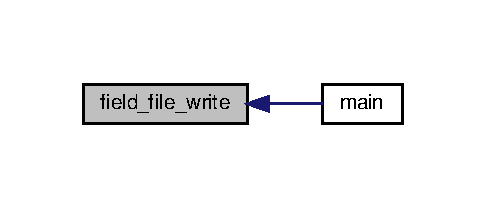
\includegraphics[width=233pt]{main_8f90_af0a1310807f21ee1a2c0fdf14c58b63b_icgraph}
\end{center}
\end{figure}
\mbox{\Hypertarget{main_8f90_a8ec2266d83cd6c0b762cbcbc92c0af3d}\label{main_8f90_a8ec2266d83cd6c0b762cbcbc92c0af3d}} 
\index{main.\+f90@{main.\+f90}!main@{main}}
\index{main@{main}!main.\+f90@{main.\+f90}}
\subsubsection{\texorpdfstring{main()}{main()}}
{\footnotesize\ttfamily program main (\begin{DoxyParamCaption}{ }\end{DoxyParamCaption})}



Main execution program for the example problem of Pa\+Sca\+L\+\_\+\+T\+D\+MA. 

Here is the call graph for this function\+:
\nopagebreak
\begin{figure}[H]
\begin{center}
\leavevmode
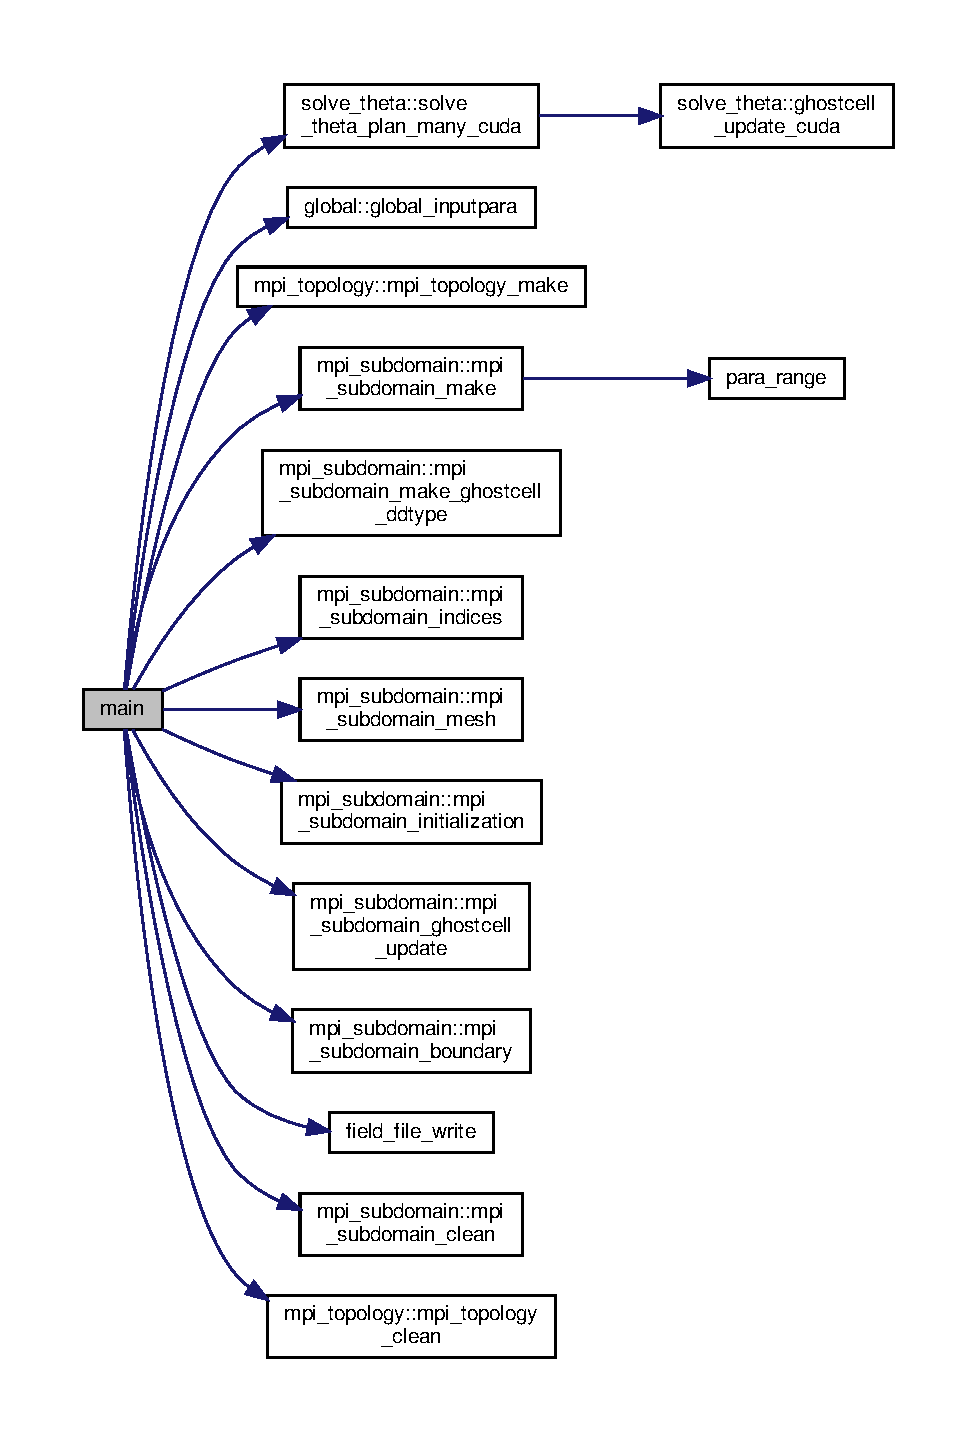
\includegraphics[width=350pt]{main_8f90_a8ec2266d83cd6c0b762cbcbc92c0af3d_cgraph}
\end{center}
\end{figure}

\hypertarget{mpi__subdomain_8f90}{}\section{/home/jihoon/\+Develop/\+Pa\+Sca\+L\+\_\+\+T\+D\+M\+A/examples/mpi\+\_\+subdomain.f90 File Reference}
\label{mpi__subdomain_8f90}\index{/home/jihoon/\+Develop/\+Pa\+Sca\+L\+\_\+\+T\+D\+M\+A/examples/mpi\+\_\+subdomain.\+f90@{/home/jihoon/\+Develop/\+Pa\+Sca\+L\+\_\+\+T\+D\+M\+A/examples/mpi\+\_\+subdomain.\+f90}}


This file contains a module of subdomains for the example problem of Pa\+Sca\+L\+\_\+\+T\+D\+MA.  


\subsection*{Modules}
\begin{DoxyCompactItemize}
\item 
module \hyperlink{namespacempi__subdomain}{mpi\+\_\+subdomain}
\begin{DoxyCompactList}\small\item\em Module for building subdomains from the physical domain. \end{DoxyCompactList}\end{DoxyCompactItemize}
\subsection*{Functions/\+Subroutines}
\begin{DoxyCompactItemize}
\item 
subroutine, public \hyperlink{namespacempi__subdomain_a3a1e7cf64aafbebd3c09b92fc56bd311}{mpi\+\_\+subdomain\+::mpi\+\_\+subdomain\+\_\+make} (nprocs\+\_\+in\+\_\+x, myrank\+\_\+in\+\_\+x, nprocs\+\_\+in\+\_\+y, myrank\+\_\+in\+\_\+y, nprocs\+\_\+in\+\_\+z, myrank\+\_\+in\+\_\+z)
\begin{DoxyCompactList}\small\item\em Prepare the subdomain and determine the size of the subdomain. \end{DoxyCompactList}\item 
subroutine, public \hyperlink{namespacempi__subdomain_a56e9f2afd59e45fcada0f1c21a90eefe}{mpi\+\_\+subdomain\+::mpi\+\_\+subdomain\+\_\+clean}
\begin{DoxyCompactList}\small\item\em Deallocate subdomain variables. \end{DoxyCompactList}\item 
subroutine, public \hyperlink{namespacempi__subdomain_ad788c273d92ea7058caf0874bffdad6d}{mpi\+\_\+subdomain\+::mpi\+\_\+subdomain\+\_\+make\+\_\+ghostcell\+\_\+ddtype}
\begin{DoxyCompactList}\small\item\em Build derived datatypes for subdomain communication using ghostcells. \end{DoxyCompactList}\item 
subroutine, public \hyperlink{namespacempi__subdomain_a2e34a77537009dd448375e8fdc8d5b62}{mpi\+\_\+subdomain\+::mpi\+\_\+subdomain\+\_\+ghostcell\+\_\+update} (theta\+\_\+sub, comm\+\_\+1d\+\_\+x, comm\+\_\+1d\+\_\+y, comm\+\_\+1d\+\_\+z)
\begin{DoxyCompactList}\small\item\em Update the values of boundary ghostcells through communication in all directions. \end{DoxyCompactList}\item 
subroutine, public \hyperlink{namespacempi__subdomain_afe948dc18da021f2448cf9a6265155fe}{mpi\+\_\+subdomain\+::mpi\+\_\+subdomain\+\_\+indices} (myrank\+\_\+in\+\_\+y, nprocs\+\_\+in\+\_\+y)
\begin{DoxyCompactList}\small\item\em Determine whether the next grids are empty(0) or not(1) only in the y-\/direction. \end{DoxyCompactList}\item 
subroutine, public \hyperlink{namespacempi__subdomain_a612331eead74041f174ece9a572c7427}{mpi\+\_\+subdomain\+::mpi\+\_\+subdomain\+\_\+mesh} (myrank\+\_\+in\+\_\+x, myrank\+\_\+in\+\_\+y, myrank\+\_\+in\+\_\+z, nprocs\+\_\+in\+\_\+x, nprocs\+\_\+in\+\_\+y, nprocs\+\_\+in\+\_\+z)
\begin{DoxyCompactList}\small\item\em Assign grid coordinates and lengths of subdomains. \end{DoxyCompactList}\item 
subroutine, public \hyperlink{namespacempi__subdomain_a7cc0deb85b84358eb7addeea849733c4}{mpi\+\_\+subdomain\+::mpi\+\_\+subdomain\+\_\+initialization} (theta\+\_\+sub, myrank\+\_\+in\+\_\+y, nprocs\+\_\+in\+\_\+y)
\begin{DoxyCompactList}\small\item\em Initialize the values of the main variable in a subdomain. \end{DoxyCompactList}\item 
subroutine, public \hyperlink{namespacempi__subdomain_a55659431068678c08d21847338390ea8}{mpi\+\_\+subdomain\+::mpi\+\_\+subdomain\+\_\+boundary} (theta\+\_\+sub, myrank\+\_\+in\+\_\+y, nprocs\+\_\+in\+\_\+y)
\begin{DoxyCompactList}\small\item\em Assign the values of boundary grids in the subdomain. \end{DoxyCompactList}\end{DoxyCompactItemize}
\subsection*{Variables}
\begin{DoxyCompactItemize}
\item 
integer \hyperlink{namespacempi__subdomain_acd16f258caed20a7d8d38cd28ae64688}{mpi\+\_\+subdomain\+::ierr}
\item 
double precision, dimension(\+:,\+:), allocatable, public \hyperlink{namespacempi__subdomain_ad61f27caf5f32301a077e21363c2d73b}{mpi\+\_\+subdomain\+::thetabc3\+\_\+sub}
\begin{DoxyCompactList}\small\item\em B.\+C. of lower wall. \end{DoxyCompactList}\item 
double precision, dimension(\+:,\+:), allocatable, public \hyperlink{namespacempi__subdomain_ad1705bede0c0d39ad16f9f94afe32be6}{mpi\+\_\+subdomain\+::thetabc4\+\_\+sub}
\begin{DoxyCompactList}\small\item\em B.\+C. of upper wall. \end{DoxyCompactList}\item 
integer, dimension(\+:), allocatable, public \hyperlink{namespacempi__subdomain_ac22380b1c941dd6c53cabe7287d185e9}{mpi\+\_\+subdomain\+::jmbc\+\_\+index}
\begin{DoxyCompactList}\small\item\em Flag whether lower grid is empty(0) or not. \end{DoxyCompactList}\item 
integer, dimension(\+:), allocatable, public \hyperlink{namespacempi__subdomain_a9adbfdd11c7e9fdb968bb8eef2b13c2b}{mpi\+\_\+subdomain\+::jpbc\+\_\+index}
\begin{DoxyCompactList}\small\item\em Flag whether upper grid is empty(0) or not. \end{DoxyCompactList}\end{DoxyCompactItemize}
\textbf{ }\par
\begin{DoxyCompactItemize}
\item 
integer, public \hyperlink{namespacempi__subdomain_a005fe127fe0fc85b932814a820a36444}{mpi\+\_\+subdomain\+::nx\+\_\+sub}
\begin{DoxyCompactList}\small\item\em Grid numbers in the subdomain. \end{DoxyCompactList}\item 
integer, public \hyperlink{namespacempi__subdomain_a665ba05d0ae9309dd28b9b513a0c87a1}{mpi\+\_\+subdomain\+::ny\+\_\+sub}
\item 
integer, public \hyperlink{namespacempi__subdomain_a07555cc931ac78376a4c81207662251f}{mpi\+\_\+subdomain\+::nz\+\_\+sub}
\end{DoxyCompactItemize}

\textbf{ }\par
\begin{DoxyCompactItemize}
\item 
integer, public \hyperlink{namespacempi__subdomain_ab8925faaa6f45326c1d11efa37e03566}{mpi\+\_\+subdomain\+::ista}
\begin{DoxyCompactList}\small\item\em Grid indices of the assigned range. \end{DoxyCompactList}\item 
integer, public \hyperlink{namespacempi__subdomain_abbd7d35107c53bcfd2b2b52771f4aa67}{mpi\+\_\+subdomain\+::iend}
\item 
integer, public \hyperlink{namespacempi__subdomain_ac85bfba1caf77f9c3c0047fe9450fee6}{mpi\+\_\+subdomain\+::jsta}
\item 
integer, public \hyperlink{namespacempi__subdomain_a06433a0d1a081c51202a0010c21c9d36}{mpi\+\_\+subdomain\+::jend}
\item 
integer, public \hyperlink{namespacempi__subdomain_acd499eb1d07159aa9f5c878f9519b00f}{mpi\+\_\+subdomain\+::ksta}
\item 
integer, public \hyperlink{namespacempi__subdomain_af9934313b1ccbcb09f30916df3326076}{mpi\+\_\+subdomain\+::kend}
\end{DoxyCompactItemize}

\textbf{ }\par
\begin{DoxyCompactItemize}
\item 
double precision, dimension(\+:), allocatable, public \hyperlink{namespacempi__subdomain_a978554e1520c79471ef3793ed1872b37}{mpi\+\_\+subdomain\+::x\+\_\+sub}
\begin{DoxyCompactList}\small\item\em Coordinates of grid points in the subdomain. \end{DoxyCompactList}\item 
double precision, dimension(\+:), allocatable, public \hyperlink{namespacempi__subdomain_a58b09abee5f1002de7b20b1b86f5c821}{mpi\+\_\+subdomain\+::y\+\_\+sub}
\item 
double precision, dimension(\+:), allocatable, public \hyperlink{namespacempi__subdomain_aab6d78e49471a9a3db5ad9df4c3d4041}{mpi\+\_\+subdomain\+::z\+\_\+sub}
\end{DoxyCompactItemize}

\textbf{ }\par
\begin{DoxyCompactItemize}
\item 
double precision, dimension(\+:), allocatable, public \hyperlink{namespacempi__subdomain_a56af1740899dc9df6868e5e71a0884a5}{mpi\+\_\+subdomain\+::dmx\+\_\+sub}
\begin{DoxyCompactList}\small\item\em Grid lengths in the subdomain. \end{DoxyCompactList}\item 
double precision, dimension(\+:), allocatable, public \hyperlink{namespacempi__subdomain_ae44efbff9669bfad03a79ab41b5e8ace}{mpi\+\_\+subdomain\+::dmy\+\_\+sub}
\item 
double precision, dimension(\+:), allocatable, public \hyperlink{namespacempi__subdomain_afb6341d7362587d6fd0a06fe78ba4e3f}{mpi\+\_\+subdomain\+::dmz\+\_\+sub}
\end{DoxyCompactItemize}

\textbf{ }\par
\begin{DoxyCompactItemize}
\item 
integer \hyperlink{namespacempi__subdomain_a93395266b1630e5a91e8e89531dfcec6}{mpi\+\_\+subdomain\+::ddtype\+\_\+sendto\+\_\+e}
\begin{DoxyCompactList}\small\item\em Derived datatype for communication between x-\/neighbor subdomains. \end{DoxyCompactList}\item 
integer \hyperlink{namespacempi__subdomain_a0b2a4ab6d6a88a3817f473a5c2c172b9}{mpi\+\_\+subdomain\+::ddtype\+\_\+recvfrom\+\_\+w}
\item 
integer \hyperlink{namespacempi__subdomain_a0701fde01daea1a6fd51b62c75b8ee82}{mpi\+\_\+subdomain\+::ddtype\+\_\+sendto\+\_\+w}
\item 
integer \hyperlink{namespacempi__subdomain_a18a84c0f3ca27cd4dd73057ff035f341}{mpi\+\_\+subdomain\+::ddtype\+\_\+recvfrom\+\_\+e}
\end{DoxyCompactItemize}

\textbf{ }\par
\begin{DoxyCompactItemize}
\item 
integer \hyperlink{namespacempi__subdomain_a55f5c1af9bd941fd176e619bddbb8d82}{mpi\+\_\+subdomain\+::ddtype\+\_\+sendto\+\_\+n}
\begin{DoxyCompactList}\small\item\em Derived datatype for communication between y-\/neighbor subdomains. \end{DoxyCompactList}\item 
integer \hyperlink{namespacempi__subdomain_a1f46916f08758533cad3ecac33233e38}{mpi\+\_\+subdomain\+::ddtype\+\_\+recvfrom\+\_\+s}
\item 
integer \hyperlink{namespacempi__subdomain_a660f83d621188fb7eb60ad10eab4c9b5}{mpi\+\_\+subdomain\+::ddtype\+\_\+sendto\+\_\+s}
\item 
integer \hyperlink{namespacempi__subdomain_a74f1edb3c9227692b250285680518dc4}{mpi\+\_\+subdomain\+::ddtype\+\_\+recvfrom\+\_\+n}
\end{DoxyCompactItemize}

\textbf{ }\par
\begin{DoxyCompactItemize}
\item 
integer \hyperlink{namespacempi__subdomain_a4f3d66535b947c7afee75e6e73a47206}{mpi\+\_\+subdomain\+::ddtype\+\_\+sendto\+\_\+f}
\begin{DoxyCompactList}\small\item\em Derived datatype for communication between z-\/neighbor subdomains. \end{DoxyCompactList}\item 
integer \hyperlink{namespacempi__subdomain_ad6462f18c8c68c076005957e9d062252}{mpi\+\_\+subdomain\+::ddtype\+\_\+recvfrom\+\_\+b}
\item 
integer \hyperlink{namespacempi__subdomain_a7a2af0322a7aaa435951a5432859687a}{mpi\+\_\+subdomain\+::ddtype\+\_\+sendto\+\_\+b}
\item 
integer \hyperlink{namespacempi__subdomain_a4da19838e8bc3934ad5c24db424bec2c}{mpi\+\_\+subdomain\+::ddtype\+\_\+recvfrom\+\_\+f}
\end{DoxyCompactItemize}



\subsection{Detailed Description}
This file contains a module of subdomains for the example problem of Pa\+Sca\+L\+\_\+\+T\+D\+MA. 

The target example problem is the three-\/dimensional(3D) time-\/dependent heat conduction problem in a unit cube domain applied with the boundary conditions of vertically constant temperature and horizontally periodic boundaries. \begin{DoxyAuthor}{Author}

\begin{DoxyItemize}
\item Kiha Kim (\href{mailto:k-kiha@yonsei.ac.kr}{\tt k-\/kiha@yonsei.\+ac.\+kr}), Department of Computational Science \& Engineering, Yonsei University
\item Ji-\/\+Hoon Kang (\href{mailto:jhkang@kisti.re.kr}{\tt jhkang@kisti.\+re.\+kr}), Korea Institute of Science and Technology Information
\item Jung-\/\+Il Choi (\href{mailto:jic@yonsei.ac.kr}{\tt jic@yonsei.\+ac.\+kr}), Department of Computational Science \& Engineering, Yonsei University
\end{DoxyItemize}
\end{DoxyAuthor}
\begin{DoxyDate}{Date}
March 2023 
\end{DoxyDate}
\begin{DoxyVersion}{Version}
2.\+0 
\end{DoxyVersion}
\begin{DoxyParagraph}{Copyright}
Copyright (c) 2019-\/2023 Kiha Kim and Jung-\/\+Il choi, Yonsei University and Ji-\/\+Hoon Kang, Korea Institute of Science and Technology Information, All rights reserved. 
\end{DoxyParagraph}
\begin{DoxyParagraph}{License }
This project is release under the terms of the M\+IT License (see L\+I\+C\+E\+N\+SE in ) 
\end{DoxyParagraph}

\hypertarget{mpi__topology_8f90}{}\section{/home/jihoon/\+Develop/\+Pa\+Sca\+L\+\_\+\+T\+D\+M\+A/examples/mpi\+\_\+topology.f90 File Reference}
\label{mpi__topology_8f90}\index{/home/jihoon/\+Develop/\+Pa\+Sca\+L\+\_\+\+T\+D\+M\+A/examples/mpi\+\_\+topology.\+f90@{/home/jihoon/\+Develop/\+Pa\+Sca\+L\+\_\+\+T\+D\+M\+A/examples/mpi\+\_\+topology.\+f90}}


This file contains a module of communication topology for the example problem of Pa\+Sca\+L\+\_\+\+T\+D\+MA.  


\subsection*{Data Types}
\begin{DoxyCompactItemize}
\item 
type \hyperlink{structmpi__topology_1_1cart__comm__1d}{mpi\+\_\+topology\+::cart\+\_\+comm\+\_\+1d}
\begin{DoxyCompactList}\small\item\em Type variable for the information of 1D communicator. \end{DoxyCompactList}\end{DoxyCompactItemize}
\subsection*{Modules}
\begin{DoxyCompactItemize}
\item 
module \hyperlink{namespacempi__topology}{mpi\+\_\+topology}
\begin{DoxyCompactList}\small\item\em Module for creating the cartesian topology of the M\+PI processes and subcommunicators. \end{DoxyCompactList}\end{DoxyCompactItemize}
\subsection*{Functions/\+Subroutines}
\begin{DoxyCompactItemize}
\item 
subroutine, public \hyperlink{namespacempi__topology_aa14e91baaec6d1c1082ebd5ac6e19128}{mpi\+\_\+topology\+::mpi\+\_\+topology\+\_\+clean} ()
\begin{DoxyCompactList}\small\item\em Destroy the communicator for cartesian topology. \end{DoxyCompactList}\item 
subroutine, public \hyperlink{namespacempi__topology_a8819f16f50aded913f17520a29d3ec4c}{mpi\+\_\+topology\+::mpi\+\_\+topology\+\_\+make} ()
\begin{DoxyCompactList}\small\item\em Create the cartesian topology for the M\+PI processes and subcommunicators. \end{DoxyCompactList}\end{DoxyCompactItemize}
\subsection*{Variables}
\begin{DoxyCompactItemize}
\item 
integer, public \hyperlink{namespacempi__topology_a2b10bc780ba4b14ea773c36f3e489a94}{mpi\+\_\+topology\+::mpi\+\_\+world\+\_\+cart}
\begin{DoxyCompactList}\small\item\em Communicator for cartesian topology. \end{DoxyCompactList}\item 
integer, dimension(0\+:2), public \hyperlink{namespacempi__topology_ac837e97cb4896a72d94eb7a9f12d6682}{mpi\+\_\+topology\+::np\+\_\+dim}
\begin{DoxyCompactList}\small\item\em Number of M\+PI processes in 3D topology. \end{DoxyCompactList}\item 
logical, dimension(0\+:2), public \hyperlink{namespacempi__topology_ac24cb383bdfbdf566165cf78b03677aa}{mpi\+\_\+topology\+::period}
\begin{DoxyCompactList}\small\item\em Periodicity in each direction. \end{DoxyCompactList}\item 
type(cart\+\_\+comm\+\_\+1d), public \hyperlink{namespacempi__topology_a4ef8d80f442649d77707d5ebeeefa391}{mpi\+\_\+topology\+::comm\+\_\+1d\+\_\+x}
\begin{DoxyCompactList}\small\item\em Subcommunicator information in x-\/direction. \end{DoxyCompactList}\item 
type(cart\+\_\+comm\+\_\+1d), public \hyperlink{namespacempi__topology_ad48a88602b9b9950200733823f95b5d0}{mpi\+\_\+topology\+::comm\+\_\+1d\+\_\+y}
\begin{DoxyCompactList}\small\item\em Subcommunicator information in y-\/direction. \end{DoxyCompactList}\item 
type(cart\+\_\+comm\+\_\+1d), public \hyperlink{namespacempi__topology_aed5c66dd4697b116c53db4613ad802ce}{mpi\+\_\+topology\+::comm\+\_\+1d\+\_\+z}
\begin{DoxyCompactList}\small\item\em Subcommunicator information in z-\/direction. \end{DoxyCompactList}\end{DoxyCompactItemize}


\subsection{Detailed Description}
This file contains a module of communication topology for the example problem of Pa\+Sca\+L\+\_\+\+T\+D\+MA. 

The target example problem is the three-\/dimensional time-\/dependent heat conduction problem in a unit cube domain applied with the boundary conditions of vertically constant temperature and horizontally periodic boundaries. \begin{DoxyAuthor}{Author}

\begin{DoxyItemize}
\item Kiha Kim (\href{mailto:k-kiha@yonsei.ac.kr}{\tt k-\/kiha@yonsei.\+ac.\+kr}), Department of Computational Science \& Engineering, Yonsei University
\item Ji-\/\+Hoon Kang (\href{mailto:jhkang@kisti.re.kr}{\tt jhkang@kisti.\+re.\+kr}), Korea Institute of Science and Technology Information
\item Jung-\/\+Il Choi (\href{mailto:jic@yonsei.ac.kr}{\tt jic@yonsei.\+ac.\+kr}), Department of Computational Science \& Engineering, Yonsei University
\end{DoxyItemize}
\end{DoxyAuthor}
\begin{DoxyDate}{Date}
March 2023 
\end{DoxyDate}
\begin{DoxyVersion}{Version}
2.\+0 
\end{DoxyVersion}
\begin{DoxyParagraph}{Copyright}
Copyright (c) 2019-\/2023 Kiha Kim and Jung-\/\+Il choi, Yonsei University and Ji-\/\+Hoon Kang, Korea Institute of Science and Technology Information, All rights reserved. 
\end{DoxyParagraph}
\begin{DoxyParagraph}{License }
This project is release under the terms of the M\+IT License (see L\+I\+C\+E\+N\+SE in ) 
\end{DoxyParagraph}

\hypertarget{solve__theta_8f90}{}\section{/home/jihoon/\+Develop/\+Pa\+Sca\+L\+\_\+\+T\+D\+M\+A/examples/solve\+\_\+theta.f90 File Reference}
\label{solve__theta_8f90}\index{/home/jihoon/\+Develop/\+Pa\+Sca\+L\+\_\+\+T\+D\+M\+A/examples/solve\+\_\+theta.\+f90@{/home/jihoon/\+Develop/\+Pa\+Sca\+L\+\_\+\+T\+D\+M\+A/examples/solve\+\_\+theta.\+f90}}


This file contains a solver subroutine for the example problem of Pa\+Sca\+L\+\_\+\+T\+D\+MA.  


\subsection*{Modules}
\begin{DoxyCompactItemize}
\item 
module \hyperlink{namespacesolve__theta}{solve\+\_\+theta}
\end{DoxyCompactItemize}
\subsection*{Functions/\+Subroutines}
\begin{DoxyCompactItemize}
\item 
subroutine, public \hyperlink{namespacesolve__theta_a215d44e312ec3ab2a3ab44fa0613b100}{solve\+\_\+theta\+::solve\+\_\+theta\+\_\+plan\+\_\+single} (theta)
\begin{DoxyCompactList}\small\item\em An example solver for a single tridiagonal system of equations using Pa\+Sca\+L\+\_\+\+T\+D\+MA. \end{DoxyCompactList}\item 
subroutine, public \hyperlink{namespacesolve__theta_a0b7fdb576c007dc344092bf40efb0f4b}{solve\+\_\+theta\+::solve\+\_\+theta\+\_\+plan\+\_\+many} (theta)
\begin{DoxyCompactList}\small\item\em An example solver for many tridiagonal systems of equations using Pa\+Sca\+L\+\_\+\+T\+D\+MA. \end{DoxyCompactList}\item 
subroutine, public \hyperlink{namespacesolve__theta_a84c4bdc671112259790470f6ad4c7e4c}{solve\+\_\+theta\+::solve\+\_\+theta\+\_\+plan\+\_\+many\+\_\+cuda} (theta)
\begin{DoxyCompactList}\small\item\em An example solver for many tridiagonal systems of equations using Pa\+Sca\+L\+\_\+\+T\+D\+MA with C\+U\+DA. \end{DoxyCompactList}\item 
subroutine \hyperlink{namespacesolve__theta_a75284cf6dd015edde5309be8368c4c9e}{solve\+\_\+theta\+::ghostcell\+\_\+update\+\_\+cuda} (Value\+\_\+sub\+\_\+d)
\begin{DoxyCompactList}\small\item\em Ghost cell update in device. \end{DoxyCompactList}\end{DoxyCompactItemize}


\subsection{Detailed Description}
This file contains a solver subroutine for the example problem of Pa\+Sca\+L\+\_\+\+T\+D\+MA. 

The target example problem is the three-\/dimensional time-\/dependent heat conduction problem in a unit cube domain applied with the boundary conditions of vertically constant temperature and horizontally periodic boundaries. \begin{DoxyAuthor}{Author}

\begin{DoxyItemize}
\item Kiha Kim (\href{mailto:k-kiha@yonsei.ac.kr}{\tt k-\/kiha@yonsei.\+ac.\+kr}), Department of Computational Science \& Engineering, Yonsei University
\item Ji-\/\+Hoon Kang (\href{mailto:jhkang@kisti.re.kr}{\tt jhkang@kisti.\+re.\+kr}), Korea Institute of Science and Technology Information
\item Mingyu Yang (\href{mailto:yang926@yonsei.ac.kr}{\tt yang926@yonsei.\+ac.\+kr}), Multi-\/\+Physics Modeling and Computation Lab., Yonsei University
\item Jung-\/\+Il Choi (\href{mailto:jic@yonsei.ac.kr}{\tt jic@yonsei.\+ac.\+kr}), Department of Computational Science \& Engineering, Yonsei University
\end{DoxyItemize}
\end{DoxyAuthor}
\begin{DoxyDate}{Date}
March 2023 
\end{DoxyDate}
\begin{DoxyVersion}{Version}
2.\+0 
\end{DoxyVersion}
\begin{DoxyParagraph}{Copyright}
Copyright (c) 2019-\/2023 Kiha Kim, Mingyu Yang and Jung-\/\+Il choi, Yonsei University and Ji-\/\+Hoon Kang, Korea Institute of Science and Technology Information, All rights reserved. 
\end{DoxyParagraph}
\begin{DoxyParagraph}{License }
This project is release under the terms of the M\+IT License (see L\+I\+C\+E\+N\+SE in ) 
\end{DoxyParagraph}

\hypertarget{_makefile_8inc}{}\section{/home/jihoon/\+Develop/\+Pa\+Sca\+L\+\_\+\+T\+D\+M\+A/\+Makefile.inc File Reference}
\label{_makefile_8inc}\index{/home/jihoon/\+Develop/\+Pa\+Sca\+L\+\_\+\+T\+D\+M\+A/\+Makefile.\+inc@{/home/jihoon/\+Develop/\+Pa\+Sca\+L\+\_\+\+T\+D\+M\+A/\+Makefile.\+inc}}

\hypertarget{_r_e_a_d_m_e_8md}{}\section{/home/jihoon/\+Develop/\+Pa\+Sca\+L\+\_\+\+T\+D\+M\+A/\+R\+E\+A\+D\+ME.md File Reference}
\label{_r_e_a_d_m_e_8md}\index{/home/jihoon/\+Develop/\+Pa\+Sca\+L\+\_\+\+T\+D\+M\+A/\+R\+E\+A\+D\+M\+E.\+md@{/home/jihoon/\+Develop/\+Pa\+Sca\+L\+\_\+\+T\+D\+M\+A/\+R\+E\+A\+D\+M\+E.\+md}}

\hypertarget{nvtx_8f90}{}\section{/home/jihoon/\+Develop/\+Pa\+Sca\+L\+\_\+\+T\+D\+M\+A/src/nvtx.f90 File Reference}
\label{nvtx_8f90}\index{/home/jihoon/\+Develop/\+Pa\+Sca\+L\+\_\+\+T\+D\+M\+A/src/nvtx.\+f90@{/home/jihoon/\+Develop/\+Pa\+Sca\+L\+\_\+\+T\+D\+M\+A/src/nvtx.\+f90}}
\subsection*{Data Types}
\begin{DoxyCompactItemize}
\item 
type \hyperlink{structnvtx_1_1nvtxeventattributes}{nvtx\+::nvtxeventattributes}
\item 
interface \hyperlink{interfacenvtx_1_1nvtxrangepush}{nvtx\+::nvtxrangepush}
\item 
interface \hyperlink{interfacenvtx_1_1nvtxrangepop}{nvtx\+::nvtxrangepop}
\end{DoxyCompactItemize}
\subsection*{Modules}
\begin{DoxyCompactItemize}
\item 
module \hyperlink{namespacenvtx}{nvtx}
\end{DoxyCompactItemize}
\subsection*{Functions/\+Subroutines}
\begin{DoxyCompactItemize}
\item 
subroutine \hyperlink{namespacenvtx_abaf43be3229e42bd0f4c1e75d9670075}{nvtx\+::nvtxstartrange} (name, id)
\item 
subroutine \hyperlink{namespacenvtx_aed9b06c5398e0a5b8d7a6e687564fb46}{nvtx\+::nvtxendrange}
\end{DoxyCompactItemize}

\hypertarget{para__range_8f90}{}\section{/home/jihoon/\+Develop/\+Pa\+Sca\+L\+\_\+\+T\+D\+M\+A/src/para\+\_\+range.f90 File Reference}
\label{para__range_8f90}\index{/home/jihoon/\+Develop/\+Pa\+Sca\+L\+\_\+\+T\+D\+M\+A/src/para\+\_\+range.\+f90@{/home/jihoon/\+Develop/\+Pa\+Sca\+L\+\_\+\+T\+D\+M\+A/src/para\+\_\+range.\+f90}}


The para\+\_\+range function assigns the computing range to each M\+PI process.  


\subsection*{Functions/\+Subroutines}
\begin{DoxyCompactItemize}
\item 
subroutine \hyperlink{para__range_8f90_ab75ab386311975aa4ff7cac06798fcd4}{para\+\_\+range} (n1, n2, nprocs, myrank, ista, iend)
\begin{DoxyCompactList}\small\item\em Compute the indices of the assigned range for each M\+PI process . \end{DoxyCompactList}\end{DoxyCompactItemize}


\subsection{Detailed Description}
The para\+\_\+range function assigns the computing range to each M\+PI process. 

\begin{DoxyAuthor}{Author}

\begin{DoxyItemize}
\item Kiha Kim (\href{mailto:k-kiha@yonsei.ac.kr}{\tt k-\/kiha@yonsei.\+ac.\+kr}), Department of Computational Science \& Engineering, Yonsei University
\item Ji-\/\+Hoon Kang (\href{mailto:jhkang@kisti.re.kr}{\tt jhkang@kisti.\+re.\+kr}), Korea Institute of Science and Technology Information
\item Jung-\/\+Il Choi (\href{mailto:jic@yonsei.ac.kr}{\tt jic@yonsei.\+ac.\+kr}), Department of Computational Science \& Engineering, Yonsei University
\end{DoxyItemize}
\end{DoxyAuthor}
\begin{DoxyDate}{Date}
June 2019 
\end{DoxyDate}
\begin{DoxyVersion}{Version}
1.\+0 
\end{DoxyVersion}
\begin{DoxyParagraph}{Copyright}
Copyright (c) 2019-\/2023 Kiha Kim and Jung-\/\+Il choi, Yonsei University and Ji-\/\+Hoon Kang, Korea Institute of Science and Technology Information, All rights reserved. 
\end{DoxyParagraph}
\begin{DoxyParagraph}{License }
This project is release under the terms of the M\+IT License (see L\+I\+C\+E\+N\+SE in ) 
\end{DoxyParagraph}


\subsection{Function/\+Subroutine Documentation}
\mbox{\Hypertarget{para__range_8f90_ab75ab386311975aa4ff7cac06798fcd4}\label{para__range_8f90_ab75ab386311975aa4ff7cac06798fcd4}} 
\index{para\+\_\+range.\+f90@{para\+\_\+range.\+f90}!para\+\_\+range@{para\+\_\+range}}
\index{para\+\_\+range@{para\+\_\+range}!para\+\_\+range.\+f90@{para\+\_\+range.\+f90}}
\subsubsection{\texorpdfstring{para\+\_\+range()}{para\_range()}}
{\footnotesize\ttfamily subroutine para\+\_\+range (\begin{DoxyParamCaption}\item[{integer, intent(in)}]{n1,  }\item[{integer, intent(in)}]{n2,  }\item[{integer, intent(in)}]{nprocs,  }\item[{integer, intent(in)}]{myrank,  }\item[{integer, intent(out)}]{ista,  }\item[{integer, intent(out)}]{iend }\end{DoxyParamCaption})}



Compute the indices of the assigned range for each M\+PI process . 


\begin{DoxyParams}{Parameters}
{\em n1} & First index of total range \\
\hline
{\em n2} & Last index of total range \\
\hline
{\em nprocs} & Number of M\+PI process \\
\hline
{\em myrank} & Rank ID of my M\+PI process \\
\hline
{\em ista} & First index of assigned range for myrank \\
\hline
{\em iend} & Last index of assigned range for myrank \\
\hline
\end{DoxyParams}
Here is the caller graph for this function\+:
\nopagebreak
\begin{figure}[H]
\begin{center}
\leavevmode
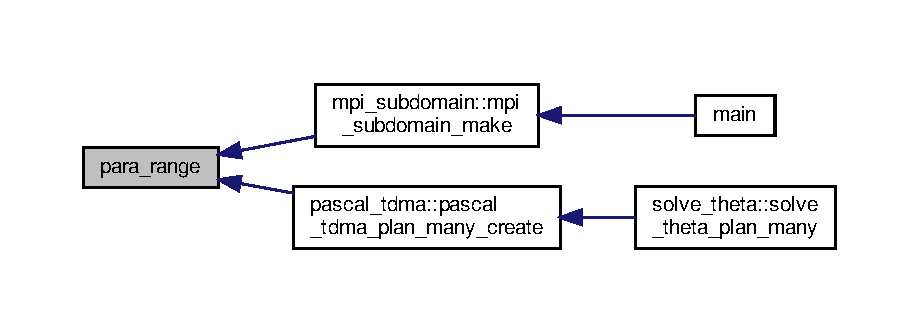
\includegraphics[width=350pt]{para__range_8f90_ab75ab386311975aa4ff7cac06798fcd4_icgraph}
\end{center}
\end{figure}

\hypertarget{pascal__tdma_8f90}{}\section{/home/jihoon/\+Develop/\+Pa\+Sca\+L\+\_\+\+T\+D\+M\+A/src/pascal\+\_\+tdma.f90 File Reference}
\label{pascal__tdma_8f90}\index{/home/jihoon/\+Develop/\+Pa\+Sca\+L\+\_\+\+T\+D\+M\+A/src/pascal\+\_\+tdma.\+f90@{/home/jihoon/\+Develop/\+Pa\+Sca\+L\+\_\+\+T\+D\+M\+A/src/pascal\+\_\+tdma.\+f90}}


Pa\+Sca\+L\+\_\+\+T\+D\+MA -\/ Parallel and Scalable Library for Tri\+Diagonal Matrix Algorithm.  


\subsection*{Data Types}
\begin{DoxyCompactItemize}
\item 
type \hyperlink{structpascal__tdma_1_1ptdma__plan__many}{pascal\+\_\+tdma\+::ptdma\+\_\+plan\+\_\+many}
\begin{DoxyCompactList}\small\item\em Execution plan for many tridiagonal systems of equations. \end{DoxyCompactList}\item 
type \hyperlink{structpascal__tdma_1_1ptdma__plan__single}{pascal\+\_\+tdma\+::ptdma\+\_\+plan\+\_\+single}
\begin{DoxyCompactList}\small\item\em Execution plan for a single tridiagonal system of equations. \end{DoxyCompactList}\end{DoxyCompactItemize}
\subsection*{Modules}
\begin{DoxyCompactItemize}
\item 
module \hyperlink{namespacepascal__tdma}{pascal\+\_\+tdma}
\begin{DoxyCompactList}\small\item\em Module for Pa\+Sca\+L-\/\+T\+D\+MA library. \end{DoxyCompactList}\end{DoxyCompactItemize}
\subsection*{Functions/\+Subroutines}
\begin{DoxyCompactItemize}
\item 
subroutine, public \hyperlink{namespacepascal__tdma_a5dfc2d7c919b47ad364a74d141532a9f}{pascal\+\_\+tdma\+::pascal\+\_\+tdma\+\_\+plan\+\_\+single\+\_\+create} (plan, myrank, nprocs, mpi\+\_\+world, gather\+\_\+rank)
\begin{DoxyCompactList}\small\item\em Create a plan for a single tridiagonal system of equations. \end{DoxyCompactList}\item 
subroutine, public \hyperlink{namespacepascal__tdma_adb04e59c740ce6c4b9518dd86eaeb594}{pascal\+\_\+tdma\+::pascal\+\_\+tdma\+\_\+plan\+\_\+single\+\_\+destroy} (plan)
\begin{DoxyCompactList}\small\item\em Deallocate the allocated arrays in the defined plan\+\_\+single . \end{DoxyCompactList}\item 
subroutine, public \hyperlink{namespacepascal__tdma_a7e9c24b343ae949044eccc8692dcc6e9}{pascal\+\_\+tdma\+::pascal\+\_\+tdma\+\_\+plan\+\_\+many\+\_\+create} (plan, n\+\_\+sys, myrank, nprocs, mpi\+\_\+world)
\begin{DoxyCompactList}\small\item\em Create a plan for many tridiagonal systems of equations. \end{DoxyCompactList}\item 
subroutine, public \hyperlink{namespacepascal__tdma_aceec478e18d25d413a5bd8a174c3fcb8}{pascal\+\_\+tdma\+::pascal\+\_\+tdma\+\_\+plan\+\_\+many\+\_\+destroy} (plan, nprocs)
\begin{DoxyCompactList}\small\item\em Destroy the allocated arrays in the defined plan\+\_\+many. \end{DoxyCompactList}\item 
subroutine, public \hyperlink{namespacepascal__tdma_ab14e132231d4b53fd65dd333ccc85a50}{pascal\+\_\+tdma\+::pascal\+\_\+tdma\+\_\+single\+\_\+solve} (plan, A, B, C, D, n\+\_\+row)
\begin{DoxyCompactList}\small\item\em Solve a single tridiagonal system of equation. \end{DoxyCompactList}\item 
subroutine, public \hyperlink{namespacepascal__tdma_ac8e377fa86c75126380f0196f6046043}{pascal\+\_\+tdma\+::pascal\+\_\+tdma\+\_\+single\+\_\+solve\+\_\+cycle} (plan, A, B, C, D, n\+\_\+row)
\begin{DoxyCompactList}\small\item\em Solve a single cyclic tridiagonal system of equations. \end{DoxyCompactList}\item 
subroutine, public \hyperlink{namespacepascal__tdma_afa0c78b8377f5fe1059907befda3c940}{pascal\+\_\+tdma\+::pascal\+\_\+tdma\+\_\+many\+\_\+solve} (plan, A, B, C, D, n\+\_\+sys, n\+\_\+row)
\begin{DoxyCompactList}\small\item\em Solve many tridiagonal systems of equations. \end{DoxyCompactList}\item 
subroutine, public \hyperlink{namespacepascal__tdma_acbaed65e67ecbfd92a8f1d51d1b69fd5}{pascal\+\_\+tdma\+::pascal\+\_\+tdma\+\_\+many\+\_\+solve\+\_\+cycle} (plan, A, B, C, D, n\+\_\+sys, n\+\_\+row)
\begin{DoxyCompactList}\small\item\em Solve many cyclic tridiagonal systems of equations. \end{DoxyCompactList}\end{DoxyCompactItemize}


\subsection{Detailed Description}
Pa\+Sca\+L\+\_\+\+T\+D\+MA -\/ Parallel and Scalable Library for Tri\+Diagonal Matrix Algorithm. 

Pa\+Scal\+\_\+\+T\+D\+MA provides an efficient and scalable computational procedure to solve many tridiagonal systems in multi-\/dimensional partial differential equations. The modified Thomas algorithm proposed by Laszlo et al.(2016) and the newly designed communication scheme have been used to reduce the communication overhead in solving many tridiagonal systems. This library is for both single and many tridiagonal systems of equations. The main algorithm for a tridiagonal matrix consists of the following five steps\+:

(1) Transform the partitioned submatrices in the tridiagonal systems into modified submatrices\+: Each computing core transforms the partitioned submatrices in the tridiagonal systems of equations into modified forms by applying the modified Thomas algorithm. (2) Construct reduced tridiagonal systems from the modified submatrices\+: The reduced tridiagonal systems are constructed by collecting the first and last rows of the modified submatrices from each core using M\+P\+I\+\_\+\+Ialltoallw. (3) Solve the reduced tridiagonal systems\+: The reduced tridiagonal systems constructed in Step 2 are solved by applying the Thomas algorithm. (4) Distribute the solutions of the reduced tridiagonal systems\+: The solutions of the reduced tridiagonal systems in Step 3 are distributed to each core using M\+P\+I\+\_\+\+Ialltoallw. This communication is an exact inverse of the communication in Step 2. (5) Update the other unknowns in the modified tridiagonal systems\+: The remaining unknowns in the modified submatrices in Step 1 are solved in each computing core using the solutions obtained in Step 3 and Step 4.

Step 1 and Step 5 are similar to the method proposed by Laszlo et al.(2016) which uses parallel cyclic reduction (P\+CR) algorithm to build and solve the reduced tridiagonal systems. Instead of using the P\+CR, we develop an all-\/to-\/all communication scheme using the M\+P\+I\+\_\+\+Ialltoall function after the modified Thomas algorithm is executed. The number of coefficients for the reduced tridiagonal systems are greatly reduced, so we can avoid the communication bandwidth problem, which is a main bottleneck for all-\/to-\/all communications. Our algorithm is also distinguished from the work of Mattor et al. (1995) which assembles the undetermined coefficients of the temporary solutions in a single processor using M\+P\+I\+\_\+\+Gather, where load imbalances are serious.

\begin{DoxyAuthor}{Author}

\begin{DoxyItemize}
\item Kiha Kim (\href{mailto:k-kiha@yonsei.ac.kr}{\tt k-\/kiha@yonsei.\+ac.\+kr}), Department of Computational Science \& Engineering, Yonsei University
\item Ji-\/\+Hoon Kang (\href{mailto:jhkang@kisti.re.kr}{\tt jhkang@kisti.\+re.\+kr}), Korea Institute of Science and Technology Information
\item Jung-\/\+Il Choi (\href{mailto:jic@yonsei.ac.kr}{\tt jic@yonsei.\+ac.\+kr}), Department of Computational Science \& Engineering, Yonsei University
\end{DoxyItemize}
\end{DoxyAuthor}
\begin{DoxyDate}{Date}
March 2023 
\end{DoxyDate}
\begin{DoxyVersion}{Version}
2.\+0 
\end{DoxyVersion}
\begin{DoxyParagraph}{Copyright}
Copyright (c) 2019-\/2023 Kiha Kim and Jung-\/\+Il choi, Yonsei University and Ji-\/\+Hoon Kang, Korea Institute of Science and Technology Information, All rights reserved. 
\end{DoxyParagraph}
\begin{DoxyParagraph}{License }
This project is released under the terms of the M\+IT License (see L\+I\+C\+E\+N\+SE ) 
\end{DoxyParagraph}

\hypertarget{pascal__tdma__cuda_8f90}{}\section{/home/jihoon/\+Develop/\+Pa\+Sca\+L\+\_\+\+T\+D\+M\+A/src/pascal\+\_\+tdma\+\_\+cuda.f90 File Reference}
\label{pascal__tdma__cuda_8f90}\index{/home/jihoon/\+Develop/\+Pa\+Sca\+L\+\_\+\+T\+D\+M\+A/src/pascal\+\_\+tdma\+\_\+cuda.\+f90@{/home/jihoon/\+Develop/\+Pa\+Sca\+L\+\_\+\+T\+D\+M\+A/src/pascal\+\_\+tdma\+\_\+cuda.\+f90}}
\subsection*{Data Types}
\begin{DoxyCompactItemize}
\item 
type \hyperlink{structpascal__tdma__cuda_1_1ptdma__plan__many__cuda}{pascal\+\_\+tdma\+\_\+cuda\+::ptdma\+\_\+plan\+\_\+many\+\_\+cuda}
\begin{DoxyCompactList}\small\item\em Execution plan for many tridiagonal systems of equations. \end{DoxyCompactList}\end{DoxyCompactItemize}
\subsection*{Modules}
\begin{DoxyCompactItemize}
\item 
module \hyperlink{namespacepascal__tdma__cuda}{pascal\+\_\+tdma\+\_\+cuda}
\begin{DoxyCompactList}\small\item\em Module for Pa\+Sca\+L\+\_\+\+T\+D\+MA library with C\+U\+DA. \end{DoxyCompactList}\end{DoxyCompactItemize}
\subsection*{Functions/\+Subroutines}
\textbf{ }\par
\begin{DoxyCompactItemize}
\item 
subroutine, public \hyperlink{namespacepascal__tdma__cuda_a84c442c238f7d1a18eef430aaa15e6c1}{pascal\+\_\+tdma\+\_\+cuda\+::pascal\+\_\+tdma\+\_\+plan\+\_\+many\+\_\+create\+\_\+cuda} (p, nx\+\_\+sys, ny\+\_\+sys, nz\+\_\+row, myrank, nprocs, mpi\+\_\+world, thread\+\_\+in)
\begin{DoxyCompactList}\small\item\em Create a plan for many tridiagonal systems of equations. \end{DoxyCompactList}\item 
subroutine, public \hyperlink{namespacepascal__tdma__cuda_a70734ba15cf5a093ac3ba2ccbc4f5330}{pascal\+\_\+tdma\+\_\+cuda\+::pascal\+\_\+tdma\+\_\+plan\+\_\+many\+\_\+destroy\+\_\+cuda} (p)
\begin{DoxyCompactList}\small\item\em Destroy the allocated arrays in the defined plan\+\_\+many. \end{DoxyCompactList}\item 
subroutine, public \hyperlink{namespacepascal__tdma__cuda_a0043d538e133925d9a37bf7bcdaf4b08}{pascal\+\_\+tdma\+\_\+cuda\+::pascal\+\_\+tdma\+\_\+many\+\_\+solve\+\_\+cuda} (p, a\+\_\+d, b\+\_\+d, c\+\_\+d, d\+\_\+d)
\begin{DoxyCompactList}\small\item\em Solve many tridiagonal systems of equations. \end{DoxyCompactList}\item 
subroutine, public \hyperlink{namespacepascal__tdma__cuda_afdd30998c4a8aecc093c823e3212b57a}{pascal\+\_\+tdma\+\_\+cuda\+::pascal\+\_\+tdma\+\_\+many\+\_\+solve\+\_\+cycle\+\_\+cuda} (p, a\+\_\+d, b\+\_\+d, c\+\_\+d, d\+\_\+d)
\begin{DoxyCompactList}\small\item\em Solve many cyclic tridiagonal systems of equations. \end{DoxyCompactList}\end{DoxyCompactItemize}


\hypertarget{tdmas_8f90}{}\section{/home/jihoon/\+Develop/\+Pa\+Sca\+L\+\_\+\+T\+D\+M\+A/src/tdmas.f90 File Reference}
\label{tdmas_8f90}\index{/home/jihoon/\+Develop/\+Pa\+Sca\+L\+\_\+\+T\+D\+M\+A/src/tdmas.\+f90@{/home/jihoon/\+Develop/\+Pa\+Sca\+L\+\_\+\+T\+D\+M\+A/src/tdmas.\+f90}}


Tridiagonal matrix (T\+DM) solvers using the Thomas algorithm.  


\subsection*{Functions/\+Subroutines}
\begin{DoxyCompactItemize}
\item 
subroutine \hyperlink{tdmas_8f90_a4a6130fff49607012fefacc8640424a7}{tdma\+\_\+single} (a, b, c, d, n1)
\begin{DoxyCompactList}\small\item\em Solve a single tridiagonal system of equations using the Thomas algorithm. \end{DoxyCompactList}\item 
subroutine \hyperlink{tdmas_8f90_a4cb1f95e9c608085c5bb19baff639d9e}{tdma\+\_\+cycl\+\_\+single} (a, b, c, d, n1)
\begin{DoxyCompactList}\small\item\em Solve a single cyclic tridiagonal system of equations using the Thomas algorithm. \end{DoxyCompactList}\item 
subroutine \hyperlink{tdmas_8f90_ab8cc761496e63e21ee8379d4fc077f05}{tdma\+\_\+many} (a, b, c, d, n1, n2)
\begin{DoxyCompactList}\small\item\em Solve many tridiagonal systems of equations using the Thomas algorithm. First index indicates the number of independent many tridiagonal systems to use vectorization. Second index indicates the row number in the tridiagonal system . \end{DoxyCompactList}\item 
subroutine \hyperlink{tdmas_8f90_a6c50d548eaa4b5e9b96ccbf8f65cb12a}{tdma\+\_\+cycl\+\_\+many} (a, b, c, d, n1, n2)
\begin{DoxyCompactList}\small\item\em Solve many cyclic tridiagonal systems of equations using the Thomas algorithm. First index indicates the number of independent many tridiagonal systems to use vectorization. Second index indicates the row number in the tridiagonal system. \end{DoxyCompactList}\end{DoxyCompactItemize}


\subsection{Detailed Description}
Tridiagonal matrix (T\+DM) solvers using the Thomas algorithm. 

A single T\+DM solver and many T\+DM solver with non-\/cyclic and cyclic conditions. \begin{DoxyAuthor}{Author}

\begin{DoxyItemize}
\item Kiha Kim (\href{mailto:k-kiha@yonsei.ac.kr}{\tt k-\/kiha@yonsei.\+ac.\+kr}), Department of Computational Science \& Engineering, Yonsei University
\item Ji-\/\+Hoon Kang (\href{mailto:jhkang@kisti.re.kr}{\tt jhkang@kisti.\+re.\+kr}), Korea Institute of Science and Technology Information
\item Jung-\/\+Il Choi (\href{mailto:jic@yonsei.ac.kr}{\tt jic@yonsei.\+ac.\+kr}), Department of Computational Science \& Engineering, Yonsei University
\end{DoxyItemize}
\end{DoxyAuthor}
\begin{DoxyDate}{Date}
March 2023 
\end{DoxyDate}
\begin{DoxyVersion}{Version}
2.\+0 
\end{DoxyVersion}
\begin{DoxyParagraph}{Copyright}
Copyright (c) 2019-\/2023 Kiha Kim and Jung-\/\+Il choi, Yonsei University and Ji-\/\+Hoon Kang, Korea Institute of Science and Technology Information, All rights reserved. 
\end{DoxyParagraph}
\begin{DoxyParagraph}{License }
This project is release under the terms of the M\+IT License (see L\+I\+C\+E\+N\+SE in ) 
\end{DoxyParagraph}


\subsection{Function/\+Subroutine Documentation}
\mbox{\Hypertarget{tdmas_8f90_a6c50d548eaa4b5e9b96ccbf8f65cb12a}\label{tdmas_8f90_a6c50d548eaa4b5e9b96ccbf8f65cb12a}} 
\index{tdmas.\+f90@{tdmas.\+f90}!tdma\+\_\+cycl\+\_\+many@{tdma\+\_\+cycl\+\_\+many}}
\index{tdma\+\_\+cycl\+\_\+many@{tdma\+\_\+cycl\+\_\+many}!tdmas.\+f90@{tdmas.\+f90}}
\subsubsection{\texorpdfstring{tdma\+\_\+cycl\+\_\+many()}{tdma\_cycl\_many()}}
{\footnotesize\ttfamily subroutine tdma\+\_\+cycl\+\_\+many (\begin{DoxyParamCaption}\item[{double precision, dimension(n1,n2), intent(inout)}]{a,  }\item[{double precision, dimension(n1,n2), intent(inout)}]{b,  }\item[{double precision, dimension(n1,n2), intent(inout)}]{c,  }\item[{double precision, dimension(n1,n2), intent(inout)}]{d,  }\item[{integer, intent(in)}]{n1,  }\item[{integer, intent(in)}]{n2 }\end{DoxyParamCaption})}



Solve many cyclic tridiagonal systems of equations using the Thomas algorithm. First index indicates the number of independent many tridiagonal systems to use vectorization. Second index indicates the row number in the tridiagonal system. 


\begin{DoxyParams}{Parameters}
{\em a} & Coefficient array in lower diagonal elements \\
\hline
{\em b} & Coefficient array in diagonal elements \\
\hline
{\em c} & Coefficient array in upper diagonal elements \\
\hline
{\em d} & Coefficient array in the right-\/hand side terms \\
\hline
{\em n1} & Number of tridiagonal systems per process \\
\hline
{\em n2} & Number of rows in each process, size of the tridiagonal matrix N divided by nprocs \\
\hline
\end{DoxyParams}
Here is the caller graph for this function\+:
\nopagebreak
\begin{figure}[H]
\begin{center}
\leavevmode
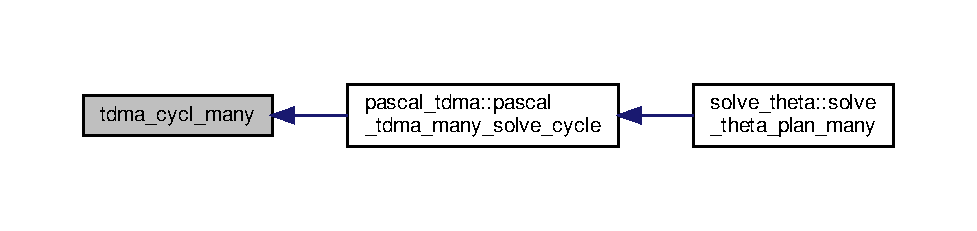
\includegraphics[width=350pt]{tdmas_8f90_a6c50d548eaa4b5e9b96ccbf8f65cb12a_icgraph}
\end{center}
\end{figure}
\mbox{\Hypertarget{tdmas_8f90_a4cb1f95e9c608085c5bb19baff639d9e}\label{tdmas_8f90_a4cb1f95e9c608085c5bb19baff639d9e}} 
\index{tdmas.\+f90@{tdmas.\+f90}!tdma\+\_\+cycl\+\_\+single@{tdma\+\_\+cycl\+\_\+single}}
\index{tdma\+\_\+cycl\+\_\+single@{tdma\+\_\+cycl\+\_\+single}!tdmas.\+f90@{tdmas.\+f90}}
\subsubsection{\texorpdfstring{tdma\+\_\+cycl\+\_\+single()}{tdma\_cycl\_single()}}
{\footnotesize\ttfamily subroutine tdma\+\_\+cycl\+\_\+single (\begin{DoxyParamCaption}\item[{double precision, dimension(n1), intent(inout)}]{a,  }\item[{double precision, dimension(n1), intent(inout)}]{b,  }\item[{double precision, dimension(n1), intent(inout)}]{c,  }\item[{double precision, dimension(n1), intent(inout)}]{d,  }\item[{integer, intent(in)}]{n1 }\end{DoxyParamCaption})}



Solve a single cyclic tridiagonal system of equations using the Thomas algorithm. 


\begin{DoxyParams}{Parameters}
{\em a} & Coefficients in lower diagonal elements \\
\hline
{\em b} & Coefficients in diagonal elements \\
\hline
{\em c} & Coefficients in upper diagonal elements \\
\hline
{\em d} & Coefficients in the right-\/hand side terms \\
\hline
{\em n1} & Number of rows in each process, dimension of tridiagonal matrix N divided by nprocs \\
\hline
\end{DoxyParams}
Here is the caller graph for this function\+:
\nopagebreak
\begin{figure}[H]
\begin{center}
\leavevmode
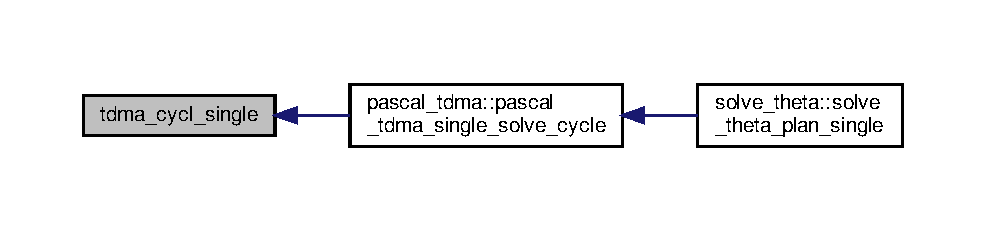
\includegraphics[width=350pt]{tdmas_8f90_a4cb1f95e9c608085c5bb19baff639d9e_icgraph}
\end{center}
\end{figure}
\mbox{\Hypertarget{tdmas_8f90_ab8cc761496e63e21ee8379d4fc077f05}\label{tdmas_8f90_ab8cc761496e63e21ee8379d4fc077f05}} 
\index{tdmas.\+f90@{tdmas.\+f90}!tdma\+\_\+many@{tdma\+\_\+many}}
\index{tdma\+\_\+many@{tdma\+\_\+many}!tdmas.\+f90@{tdmas.\+f90}}
\subsubsection{\texorpdfstring{tdma\+\_\+many()}{tdma\_many()}}
{\footnotesize\ttfamily subroutine tdma\+\_\+many (\begin{DoxyParamCaption}\item[{double precision, dimension(n1,n2), intent(inout)}]{a,  }\item[{double precision, dimension(n1,n2), intent(inout)}]{b,  }\item[{double precision, dimension(n1,n2), intent(inout)}]{c,  }\item[{double precision, dimension(n1,n2), intent(inout)}]{d,  }\item[{integer, intent(in)}]{n1,  }\item[{integer, intent(in)}]{n2 }\end{DoxyParamCaption})}



Solve many tridiagonal systems of equations using the Thomas algorithm. First index indicates the number of independent many tridiagonal systems to use vectorization. Second index indicates the row number in the tridiagonal system . 


\begin{DoxyParams}{Parameters}
{\em a} & Coefficient array in lower diagonal elements \\
\hline
{\em b} & Coefficient array in diagonal elements \\
\hline
{\em c} & Coefficient array in upper diagonal elements \\
\hline
{\em d} & Coefficient array in the right-\/hand side terms \\
\hline
{\em n1} & Number of tridiagonal systems per process \\
\hline
{\em n2} & Number of rows in each process, size of the tridiagonal matrix N divided by nprocs \\
\hline
\end{DoxyParams}
Here is the caller graph for this function\+:
\nopagebreak
\begin{figure}[H]
\begin{center}
\leavevmode
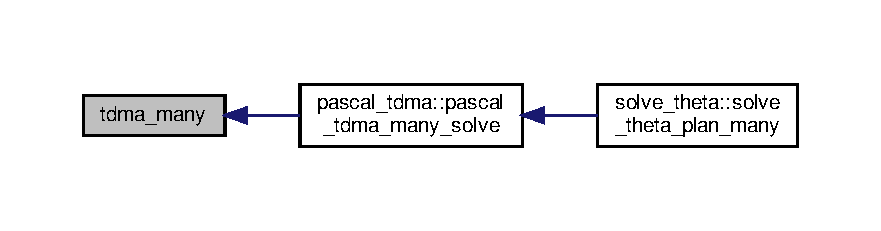
\includegraphics[width=350pt]{tdmas_8f90_ab8cc761496e63e21ee8379d4fc077f05_icgraph}
\end{center}
\end{figure}
\mbox{\Hypertarget{tdmas_8f90_a4a6130fff49607012fefacc8640424a7}\label{tdmas_8f90_a4a6130fff49607012fefacc8640424a7}} 
\index{tdmas.\+f90@{tdmas.\+f90}!tdma\+\_\+single@{tdma\+\_\+single}}
\index{tdma\+\_\+single@{tdma\+\_\+single}!tdmas.\+f90@{tdmas.\+f90}}
\subsubsection{\texorpdfstring{tdma\+\_\+single()}{tdma\_single()}}
{\footnotesize\ttfamily subroutine tdma\+\_\+single (\begin{DoxyParamCaption}\item[{double precision, dimension(n1), intent(inout)}]{a,  }\item[{double precision, dimension(n1), intent(inout)}]{b,  }\item[{double precision, dimension(n1), intent(inout)}]{c,  }\item[{double precision, dimension(n1), intent(inout)}]{d,  }\item[{integer, intent(in)}]{n1 }\end{DoxyParamCaption})}



Solve a single tridiagonal system of equations using the Thomas algorithm. 


\begin{DoxyParams}{Parameters}
{\em a} & Coefficients in lower diagonal elements \\
\hline
{\em b} & Coefficients in diagonal elements \\
\hline
{\em c} & Coefficients in upper diagonal elements \\
\hline
{\em d} & Coefficients in the right-\/hand side terms \\
\hline
{\em n1} & Number of rows in each process, dimension of tridiagonal matrix N divided by nprocs \\
\hline
\end{DoxyParams}
Here is the caller graph for this function\+:
\nopagebreak
\begin{figure}[H]
\begin{center}
\leavevmode
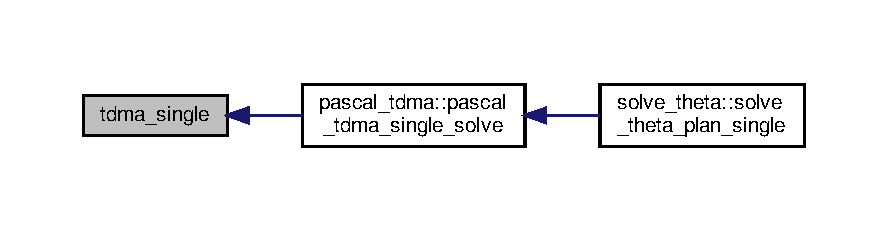
\includegraphics[width=350pt]{tdmas_8f90_a4a6130fff49607012fefacc8640424a7_icgraph}
\end{center}
\end{figure}

\hypertarget{tdmas__cuda_8f90}{}\section{/home/jihoon/\+Develop/\+Pa\+Sca\+L\+\_\+\+T\+D\+M\+A/src/tdmas\+\_\+cuda.f90 File Reference}
\label{tdmas__cuda_8f90}\index{/home/jihoon/\+Develop/\+Pa\+Sca\+L\+\_\+\+T\+D\+M\+A/src/tdmas\+\_\+cuda.\+f90@{/home/jihoon/\+Develop/\+Pa\+Sca\+L\+\_\+\+T\+D\+M\+A/src/tdmas\+\_\+cuda.\+f90}}
\subsection*{Modules}
\begin{DoxyCompactItemize}
\item 
module \hyperlink{namespacetdma}{tdma}
\end{DoxyCompactItemize}

%--- End generated contents ---

% Index
\backmatter
\newpage
\phantomsection
\clearemptydoublepage
\addcontentsline{toc}{chapter}{Index}
\printindex

\end{document}
